\batchmode
\documentclass[a4paper]{book}
\usepackage{makeidx}
\usepackage{natbib}
\usepackage{graphicx}
\usepackage{multicol}
\usepackage{float}
\usepackage{listings}
\usepackage{color}
\usepackage{ifthen}
\usepackage[table]{xcolor}
\usepackage{textcomp}
\usepackage{alltt}
\usepackage[utf8]{inputenc}
\usepackage{mathptmx}
\usepackage[scaled=.90]{helvet}
\usepackage{courier}
\usepackage{sectsty}
\usepackage[titles]{tocloft}
\usepackage{doxygen}
\lstset{language=C++,inputencoding=utf8,basicstyle=\footnotesize,breaklines=true,breakatwhitespace=true,tabsize=8,numbers=left }
\makeindex
\setcounter{tocdepth}{3}
\renewcommand{\footrulewidth}{0.4pt}
\renewcommand{\familydefault}{\sfdefault}
\hfuzz=15pt
\setlength{\emergencystretch}{15pt}
\hbadness=750
\tolerance=750
\begin{document}
\begin{titlepage}
\vspace*{7cm}
\begin{center}
{\Large lara\-\_\-rgbd }\\
\vspace*{1cm}
{\large \-Generated by Doxygen 1.7.6.1}\\
\vspace*{0.5cm}
{\small Wed Apr 23 2014 16:31:20}\\
\end{center}
\end{titlepage}
\clearemptydoublepage
\pagenumbering{roman}
\tableofcontents
\clearemptydoublepage
\pagenumbering{arabic}
\chapter{\-Main \-Page}
\label{index}

{\bfseries lara\-\_\-rgbd} 

-\/-\/$>$ 
\chapter{\-Namespace \-Index}
\section{\-Namespace \-List}
\-Here is a list of all namespaces with brief descriptions\-:\begin{DoxyCompactList}
\item\contentsline{section}{{\bf add\-\_\-pointclouds\-\_\-to\-\_\-bagfile} }{\pageref{namespaceadd__pointclouds__to__bagfile}}{}
\item\contentsline{section}{{\bf associate} }{\pageref{namespaceassociate}}{}
\item\contentsline{section}{{\bf evaluate\-\_\-ate} }{\pageref{namespaceevaluate__ate}}{}
\item\contentsline{section}{{\bf evaluate\-\_\-rpe} }{\pageref{namespaceevaluate__rpe}}{}
\item\contentsline{section}{{\bf extract\-\_\-odometry} }{\pageref{namespaceextract__odometry}}{}
\item\contentsline{section}{{\bf generate\-\_\-pointcloud} }{\pageref{namespacegenerate__pointcloud}}{}
\item\contentsline{section}{{\bf generate\-\_\-registered\-\_\-pointcloud} }{\pageref{namespacegenerate__registered__pointcloud}}{}
\item\contentsline{section}{{\bf plot\-\_\-trajectory\-\_\-into\-\_\-image} }{\pageref{namespaceplot__trajectory__into__image}}{}
\end{DoxyCompactList}

\chapter{\-Class \-Index}
\section{Class List}
Here are the classes, structs, unions and interfaces with brief descriptions\-:\begin{DoxyCompactList}
\item\contentsline{section}{\hyperlink{structVision_1_1Impl}{Vision\-::\-Impl} }{\pageref{structVision_1_1Impl}}{}
\item\contentsline{section}{\hyperlink{classVS}{V\-S} \\*\hyperlink{classVS}{V\-S}\-: vision class. Contains all vision functions and methods }{\pageref{classVS}}{}
\end{DoxyCompactList}

\chapter{\-File \-Index}
\section{\-File \-List}
\-Here is a list of all files with brief descriptions\-:\begin{DoxyCompactList}
\item\contentsline{section}{{\bf add\-\_\-pointclouds\-\_\-to\-\_\-bagfile.\-py} }{\pageref{add__pointclouds__to__bagfile_8py}}{}
\item\contentsline{section}{{\bf associate.\-py} }{\pageref{associate_8py}}{}
\item\contentsline{section}{{\bf evaluate\-\_\-ate.\-py} }{\pageref{evaluate__ate_8py}}{}
\item\contentsline{section}{{\bf evaluate\-\_\-rpe.\-py} }{\pageref{evaluate__rpe_8py}}{}
\item\contentsline{section}{{\bf extract\-\_\-odometry.\-py} }{\pageref{extract__odometry_8py}}{}
\item\contentsline{section}{{\bf generate\-\_\-pointcloud.\-py} }{\pageref{generate__pointcloud_8py}}{}
\item\contentsline{section}{{\bf generate\-\_\-registered\-\_\-pointcloud.\-py} }{\pageref{generate__registered__pointcloud_8py}}{}
\item\contentsline{section}{{\bf plot\-\_\-trajectory\-\_\-into\-\_\-image.\-py} }{\pageref{plot__trajectory__into__image_8py}}{}
\item\contentsline{section}{{\bf sensor\-\_\-processor.\-cpp} \\*
\footnotesize  
\normalsize }{\pageref{sensor__processor_8cpp}}{}
\item\contentsline{section}{{\bf sensor\-\_\-processor.\-h} }{\pageref{sensor__processor_8h}}{}
\item\contentsline{section}{{\bf sensor\-\_\-processor\-\_\-node.\-cpp} \\*\-R\-O\-S node used to process raw sensor data }{\pageref{sensor__processor__node_8cpp}}{}
\item\contentsline{section}{{\bf sensor\-\_\-processor\-\_\-node.\-h} }{\pageref{sensor__processor__node_8h}}{}
\end{DoxyCompactList}

\chapter{\-Namespace \-Documentation}
\section{add\-\_\-pointclouds\-\_\-to\-\_\-bagfile \-Namespace \-Reference}
\label{namespaceadd__pointclouds__to__bagfile}\index{add\-\_\-pointclouds\-\_\-to\-\_\-bagfile@{add\-\_\-pointclouds\-\_\-to\-\_\-bagfile}}
\subsection*{\-Variables}
\begin{DoxyCompactItemize}
\item 
tuple {\bf args} = parser.\-parse\-\_\-args()
\item 
tuple {\bf bridge} = \-Cv\-Bridge()
\item 
list {\bf buffer} = [$\,$]
\item 
list {\bf buffer\-\_\-rgb} = [$\,$]
\item 
list {\bf center\-X} = depth\-\_\-camera\-\_\-info.\-K[2]
\item 
list {\bf center\-Y} = depth\-\_\-camera\-\_\-info.\-K[5]
\item 
{\bf cortex} = \-None
\item 
tuple {\bf cv\-\_\-depth\-\_\-image} = bridge.\-imgmsg\-\_\-to\-\_\-cv({\bf depth\-\_\-image}, \char`\"{}passthrough\char`\"{})
\item 
tuple {\bf cv\-\_\-rgb\-\_\-image\-\_\-color} = bridge.\-imgmsg\-\_\-to\-\_\-cv({\bf rgb\-\_\-image\-\_\-color}, \char`\"{}bgr8\char`\"{})
\item 
tuple {\bf cv\-\_\-rgb\-\_\-image\-\_\-mono} = bridge.\-imgmsg\-\_\-to\-\_\-cv({\bf rgb\-\_\-image\-\_\-color}, \char`\"{}mono8\char`\"{})
\item 
list {\bf d} = {\bf cv\-\_\-depth\-\_\-image}[v,u]
\item 
{\bf depth\-\_\-camera\-\_\-info} = \-None
\item 
{\bf depth\-\_\-image} = \-None
\item 
tuple {\bf depth\-\_\-points} = sensor\-\_\-msgs.\-msg.\-Point\-Cloud2()
\item 
list {\bf depth\-Focal\-Length} = depth\-\_\-camera\-\_\-info.\-K[0]
\item 
int {\bf frame} = 0
\item 
{\bf imu} = {\bf msg}
\item 
tuple {\bf inbag} = rosbag.\-Bag(args.\-inputbag,'r')
\item 
tuple {\bf msg} = tf.\-msg.\-tf\-Message()
\item 
string {\bf name} = \char`\"{}x\char`\"{}
\item 
tuple {\bf nan} = float('{\bf nan}')
\item 
tuple {\bf outbag} = rosbag.\-Bag(args.\-outputbag, 'w', compression={\bf param\-\_\-compression})
\item 
{\bf param\-\_\-compression} = rosbag.\-bag.\-Compression.\-B\-Z2
\item 
tuple {\bf parser}
\item 
tuple {\bf ptx} = (u -\/ {\bf center\-X})
\item 
tuple {\bf pty} = (v -\/ {\bf center\-Y})
\item 
{\bf ptz} = {\bf d};
\item 
list {\bf rgb} = {\bf cv\-\_\-rgb\-\_\-image\-\_\-color}[v,u]
\item 
{\bf rgb\-\_\-camera\-\_\-info} = \-None
\item 
{\bf rgb\-\_\-image\-\_\-color} = \-None
\item 
tuple {\bf rgb\-\_\-image\-\_\-mono} = bridge.\-cv\-\_\-to\-\_\-imgmsg({\bf cv\-\_\-rgb\-\_\-image\-\_\-mono})
\item 
tuple {\bf rgb\-\_\-points} = sensor\-\_\-msgs.\-msg.\-Point\-Cloud2()
\item 
{\bf time\-\_\-start} = \-None
\item 
tuple {\bf transforms} = dict()
\end{DoxyCompactItemize}


\subsection{\-Variable \-Documentation}
\index{add\-\_\-pointclouds\-\_\-to\-\_\-bagfile@{add\-\_\-pointclouds\-\_\-to\-\_\-bagfile}!args@{args}}
\index{args@{args}!add_pointclouds_to_bagfile@{add\-\_\-pointclouds\-\_\-to\-\_\-bagfile}}
\subsubsection[{args}]{\setlength{\rightskip}{0pt plus 5cm}tuple {\bf add\-\_\-pointclouds\-\_\-to\-\_\-bagfile\-::args} = parser.\-parse\-\_\-args()}\label{namespaceadd__pointclouds__to__bagfile_a5e40e500d738c1b2ffa14ef759854117}


\-Definition at line 25 of file add\-\_\-pointclouds\-\_\-to\-\_\-bagfile.\-py.

\index{add\-\_\-pointclouds\-\_\-to\-\_\-bagfile@{add\-\_\-pointclouds\-\_\-to\-\_\-bagfile}!bridge@{bridge}}
\index{bridge@{bridge}!add_pointclouds_to_bagfile@{add\-\_\-pointclouds\-\_\-to\-\_\-bagfile}}
\subsubsection[{bridge}]{\setlength{\rightskip}{0pt plus 5cm}tuple {\bf add\-\_\-pointclouds\-\_\-to\-\_\-bagfile\-::bridge} = \-Cv\-Bridge()}\label{namespaceadd__pointclouds__to__bagfile_aa632b7dd5b7742688880070e337ec86c}


\-Definition at line 66 of file add\-\_\-pointclouds\-\_\-to\-\_\-bagfile.\-py.

\index{add\-\_\-pointclouds\-\_\-to\-\_\-bagfile@{add\-\_\-pointclouds\-\_\-to\-\_\-bagfile}!buffer@{buffer}}
\index{buffer@{buffer}!add_pointclouds_to_bagfile@{add\-\_\-pointclouds\-\_\-to\-\_\-bagfile}}
\subsubsection[{buffer}]{\setlength{\rightskip}{0pt plus 5cm}list {\bf add\-\_\-pointclouds\-\_\-to\-\_\-bagfile\-::buffer} = [$\,$]}\label{namespaceadd__pointclouds__to__bagfile_a0a61de89cbb8d477156b19f15f77e812}


\-Definition at line 143 of file add\-\_\-pointclouds\-\_\-to\-\_\-bagfile.\-py.

\index{add\-\_\-pointclouds\-\_\-to\-\_\-bagfile@{add\-\_\-pointclouds\-\_\-to\-\_\-bagfile}!buffer\-\_\-rgb@{buffer\-\_\-rgb}}
\index{buffer\-\_\-rgb@{buffer\-\_\-rgb}!add_pointclouds_to_bagfile@{add\-\_\-pointclouds\-\_\-to\-\_\-bagfile}}
\subsubsection[{buffer\-\_\-rgb}]{\setlength{\rightskip}{0pt plus 5cm}list {\bf add\-\_\-pointclouds\-\_\-to\-\_\-bagfile\-::buffer\-\_\-rgb} = [$\,$]}\label{namespaceadd__pointclouds__to__bagfile_aa972df9c8636792629ac72316fd66264}


\-Definition at line 144 of file add\-\_\-pointclouds\-\_\-to\-\_\-bagfile.\-py.

\index{add\-\_\-pointclouds\-\_\-to\-\_\-bagfile@{add\-\_\-pointclouds\-\_\-to\-\_\-bagfile}!center\-X@{center\-X}}
\index{center\-X@{center\-X}!add_pointclouds_to_bagfile@{add\-\_\-pointclouds\-\_\-to\-\_\-bagfile}}
\subsubsection[{center\-X}]{\setlength{\rightskip}{0pt plus 5cm}list {\bf add\-\_\-pointclouds\-\_\-to\-\_\-bagfile\-::center\-X} = depth\-\_\-camera\-\_\-info.\-K[2]}\label{namespaceadd__pointclouds__to__bagfile_a96b816cd02a6127ce33e9a95a0547f2f}


\-Definition at line 128 of file add\-\_\-pointclouds\-\_\-to\-\_\-bagfile.\-py.

\index{add\-\_\-pointclouds\-\_\-to\-\_\-bagfile@{add\-\_\-pointclouds\-\_\-to\-\_\-bagfile}!center\-Y@{center\-Y}}
\index{center\-Y@{center\-Y}!add_pointclouds_to_bagfile@{add\-\_\-pointclouds\-\_\-to\-\_\-bagfile}}
\subsubsection[{center\-Y}]{\setlength{\rightskip}{0pt plus 5cm}list {\bf add\-\_\-pointclouds\-\_\-to\-\_\-bagfile\-::center\-Y} = depth\-\_\-camera\-\_\-info.\-K[5]}\label{namespaceadd__pointclouds__to__bagfile_ad6101d2859a0e4a2201a0221bdd799e4}


\-Definition at line 129 of file add\-\_\-pointclouds\-\_\-to\-\_\-bagfile.\-py.

\index{add\-\_\-pointclouds\-\_\-to\-\_\-bagfile@{add\-\_\-pointclouds\-\_\-to\-\_\-bagfile}!cortex@{cortex}}
\index{cortex@{cortex}!add_pointclouds_to_bagfile@{add\-\_\-pointclouds\-\_\-to\-\_\-bagfile}}
\subsubsection[{cortex}]{\setlength{\rightskip}{0pt plus 5cm}{\bf add\-\_\-pointclouds\-\_\-to\-\_\-bagfile\-::cortex} = \-None}\label{namespaceadd__pointclouds__to__bagfile_acb72f4345650ea691bdd01d0ec428772}


\-Definition at line 63 of file add\-\_\-pointclouds\-\_\-to\-\_\-bagfile.\-py.

\index{add\-\_\-pointclouds\-\_\-to\-\_\-bagfile@{add\-\_\-pointclouds\-\_\-to\-\_\-bagfile}!cv\-\_\-depth\-\_\-image@{cv\-\_\-depth\-\_\-image}}
\index{cv\-\_\-depth\-\_\-image@{cv\-\_\-depth\-\_\-image}!add_pointclouds_to_bagfile@{add\-\_\-pointclouds\-\_\-to\-\_\-bagfile}}
\subsubsection[{cv\-\_\-depth\-\_\-image}]{\setlength{\rightskip}{0pt plus 5cm}tuple {\bf add\-\_\-pointclouds\-\_\-to\-\_\-bagfile\-::cv\-\_\-depth\-\_\-image} = bridge.\-imgmsg\-\_\-to\-\_\-cv({\bf depth\-\_\-image}, \char`\"{}passthrough\char`\"{})}\label{namespaceadd__pointclouds__to__bagfile_ae3f05b4dafb4feb3a14bd599fe3f9e03}


\-Definition at line 125 of file add\-\_\-pointclouds\-\_\-to\-\_\-bagfile.\-py.

\index{add\-\_\-pointclouds\-\_\-to\-\_\-bagfile@{add\-\_\-pointclouds\-\_\-to\-\_\-bagfile}!cv\-\_\-rgb\-\_\-image\-\_\-color@{cv\-\_\-rgb\-\_\-image\-\_\-color}}
\index{cv\-\_\-rgb\-\_\-image\-\_\-color@{cv\-\_\-rgb\-\_\-image\-\_\-color}!add_pointclouds_to_bagfile@{add\-\_\-pointclouds\-\_\-to\-\_\-bagfile}}
\subsubsection[{cv\-\_\-rgb\-\_\-image\-\_\-color}]{\setlength{\rightskip}{0pt plus 5cm}tuple {\bf add\-\_\-pointclouds\-\_\-to\-\_\-bagfile\-::cv\-\_\-rgb\-\_\-image\-\_\-color} = bridge.\-imgmsg\-\_\-to\-\_\-cv({\bf rgb\-\_\-image\-\_\-color}, \char`\"{}bgr8\char`\"{})}\label{namespaceadd__pointclouds__to__bagfile_af3656521d70fbd3204a6eded3944a67d}


\-Definition at line 126 of file add\-\_\-pointclouds\-\_\-to\-\_\-bagfile.\-py.

\index{add\-\_\-pointclouds\-\_\-to\-\_\-bagfile@{add\-\_\-pointclouds\-\_\-to\-\_\-bagfile}!cv\-\_\-rgb\-\_\-image\-\_\-mono@{cv\-\_\-rgb\-\_\-image\-\_\-mono}}
\index{cv\-\_\-rgb\-\_\-image\-\_\-mono@{cv\-\_\-rgb\-\_\-image\-\_\-mono}!add_pointclouds_to_bagfile@{add\-\_\-pointclouds\-\_\-to\-\_\-bagfile}}
\subsubsection[{cv\-\_\-rgb\-\_\-image\-\_\-mono}]{\setlength{\rightskip}{0pt plus 5cm}tuple {\bf add\-\_\-pointclouds\-\_\-to\-\_\-bagfile\-::cv\-\_\-rgb\-\_\-image\-\_\-mono} = bridge.\-imgmsg\-\_\-to\-\_\-cv({\bf rgb\-\_\-image\-\_\-color}, \char`\"{}mono8\char`\"{})}\label{namespaceadd__pointclouds__to__bagfile_a2403828e6736ac15f6a1d254711fa07f}


\-Definition at line 119 of file add\-\_\-pointclouds\-\_\-to\-\_\-bagfile.\-py.

\index{add\-\_\-pointclouds\-\_\-to\-\_\-bagfile@{add\-\_\-pointclouds\-\_\-to\-\_\-bagfile}!d@{d}}
\index{d@{d}!add_pointclouds_to_bagfile@{add\-\_\-pointclouds\-\_\-to\-\_\-bagfile}}
\subsubsection[{d}]{\setlength{\rightskip}{0pt plus 5cm}list {\bf add\-\_\-pointclouds\-\_\-to\-\_\-bagfile\-::d} = {\bf cv\-\_\-depth\-\_\-image}[v,u]}\label{namespaceadd__pointclouds__to__bagfile_a22296cd9d798629de5d35da0bbdb7ee1}


\-Definition at line 147 of file add\-\_\-pointclouds\-\_\-to\-\_\-bagfile.\-py.

\index{add\-\_\-pointclouds\-\_\-to\-\_\-bagfile@{add\-\_\-pointclouds\-\_\-to\-\_\-bagfile}!depth\-\_\-camera\-\_\-info@{depth\-\_\-camera\-\_\-info}}
\index{depth\-\_\-camera\-\_\-info@{depth\-\_\-camera\-\_\-info}!add_pointclouds_to_bagfile@{add\-\_\-pointclouds\-\_\-to\-\_\-bagfile}}
\subsubsection[{depth\-\_\-camera\-\_\-info}]{\setlength{\rightskip}{0pt plus 5cm}{\bf add\-\_\-pointclouds\-\_\-to\-\_\-bagfile\-::depth\-\_\-camera\-\_\-info} = \-None}\label{namespaceadd__pointclouds__to__bagfile_a1ad47849f691cb3e90e8e6c8fc50dbb2}


\-Definition at line 59 of file add\-\_\-pointclouds\-\_\-to\-\_\-bagfile.\-py.

\index{add\-\_\-pointclouds\-\_\-to\-\_\-bagfile@{add\-\_\-pointclouds\-\_\-to\-\_\-bagfile}!depth\-\_\-image@{depth\-\_\-image}}
\index{depth\-\_\-image@{depth\-\_\-image}!add_pointclouds_to_bagfile@{add\-\_\-pointclouds\-\_\-to\-\_\-bagfile}}
\subsubsection[{depth\-\_\-image}]{\setlength{\rightskip}{0pt plus 5cm}{\bf add\-\_\-pointclouds\-\_\-to\-\_\-bagfile\-::depth\-\_\-image} = \-None}\label{namespaceadd__pointclouds__to__bagfile_adc7fee14e69f0204b5f56a8be5dd9be0}


\-Definition at line 61 of file add\-\_\-pointclouds\-\_\-to\-\_\-bagfile.\-py.

\index{add\-\_\-pointclouds\-\_\-to\-\_\-bagfile@{add\-\_\-pointclouds\-\_\-to\-\_\-bagfile}!depth\-\_\-points@{depth\-\_\-points}}
\index{depth\-\_\-points@{depth\-\_\-points}!add_pointclouds_to_bagfile@{add\-\_\-pointclouds\-\_\-to\-\_\-bagfile}}
\subsubsection[{depth\-\_\-points}]{\setlength{\rightskip}{0pt plus 5cm}tuple {\bf add\-\_\-pointclouds\-\_\-to\-\_\-bagfile\-::depth\-\_\-points} = sensor\-\_\-msgs.\-msg.\-Point\-Cloud2()}\label{namespaceadd__pointclouds__to__bagfile_a06083201e4bd6d1e677352a38403f7d4}


\-Definition at line 131 of file add\-\_\-pointclouds\-\_\-to\-\_\-bagfile.\-py.

\index{add\-\_\-pointclouds\-\_\-to\-\_\-bagfile@{add\-\_\-pointclouds\-\_\-to\-\_\-bagfile}!depth\-Focal\-Length@{depth\-Focal\-Length}}
\index{depth\-Focal\-Length@{depth\-Focal\-Length}!add_pointclouds_to_bagfile@{add\-\_\-pointclouds\-\_\-to\-\_\-bagfile}}
\subsubsection[{depth\-Focal\-Length}]{\setlength{\rightskip}{0pt plus 5cm}list {\bf add\-\_\-pointclouds\-\_\-to\-\_\-bagfile\-::depth\-Focal\-Length} = depth\-\_\-camera\-\_\-info.\-K[0]}\label{namespaceadd__pointclouds__to__bagfile_a3a5613be33d4a9884988833fd2b09f4f}


\-Definition at line 130 of file add\-\_\-pointclouds\-\_\-to\-\_\-bagfile.\-py.

\index{add\-\_\-pointclouds\-\_\-to\-\_\-bagfile@{add\-\_\-pointclouds\-\_\-to\-\_\-bagfile}!frame@{frame}}
\index{frame@{frame}!add_pointclouds_to_bagfile@{add\-\_\-pointclouds\-\_\-to\-\_\-bagfile}}
\subsubsection[{frame}]{\setlength{\rightskip}{0pt plus 5cm}int {\bf add\-\_\-pointclouds\-\_\-to\-\_\-bagfile\-::frame} = 0}\label{namespaceadd__pointclouds__to__bagfile_aa3cd47715526802ae03988a17756023c}


\-Definition at line 67 of file add\-\_\-pointclouds\-\_\-to\-\_\-bagfile.\-py.

\index{add\-\_\-pointclouds\-\_\-to\-\_\-bagfile@{add\-\_\-pointclouds\-\_\-to\-\_\-bagfile}!imu@{imu}}
\index{imu@{imu}!add_pointclouds_to_bagfile@{add\-\_\-pointclouds\-\_\-to\-\_\-bagfile}}
\subsubsection[{imu}]{\setlength{\rightskip}{0pt plus 5cm}{\bf add\-\_\-pointclouds\-\_\-to\-\_\-bagfile\-::imu} = {\bf msg}}\label{namespaceadd__pointclouds__to__bagfile_a2fa7194e814a8fb414272366736c7072}


\-Definition at line 84 of file add\-\_\-pointclouds\-\_\-to\-\_\-bagfile.\-py.

\index{add\-\_\-pointclouds\-\_\-to\-\_\-bagfile@{add\-\_\-pointclouds\-\_\-to\-\_\-bagfile}!inbag@{inbag}}
\index{inbag@{inbag}!add_pointclouds_to_bagfile@{add\-\_\-pointclouds\-\_\-to\-\_\-bagfile}}
\subsubsection[{inbag}]{\setlength{\rightskip}{0pt plus 5cm}tuple {\bf add\-\_\-pointclouds\-\_\-to\-\_\-bagfile\-::inbag} = rosbag.\-Bag(args.\-inputbag,'r')}\label{namespaceadd__pointclouds__to__bagfile_ad8dd345cee6d9290060f75ee27a98027}


\-Definition at line 51 of file add\-\_\-pointclouds\-\_\-to\-\_\-bagfile.\-py.

\index{add\-\_\-pointclouds\-\_\-to\-\_\-bagfile@{add\-\_\-pointclouds\-\_\-to\-\_\-bagfile}!msg@{msg}}
\index{msg@{msg}!add_pointclouds_to_bagfile@{add\-\_\-pointclouds\-\_\-to\-\_\-bagfile}}
\subsubsection[{msg}]{\setlength{\rightskip}{0pt plus 5cm}tuple {\bf add\-\_\-pointclouds\-\_\-to\-\_\-bagfile\-::msg} = tf.\-msg.\-tf\-Message()}\label{namespaceadd__pointclouds__to__bagfile_a34da84fa8322a694b4fa257d5c06edad}


\-Definition at line 108 of file add\-\_\-pointclouds\-\_\-to\-\_\-bagfile.\-py.

\index{add\-\_\-pointclouds\-\_\-to\-\_\-bagfile@{add\-\_\-pointclouds\-\_\-to\-\_\-bagfile}!name@{name}}
\index{name@{name}!add_pointclouds_to_bagfile@{add\-\_\-pointclouds\-\_\-to\-\_\-bagfile}}
\subsubsection[{name}]{\setlength{\rightskip}{0pt plus 5cm}string {\bf add\-\_\-pointclouds\-\_\-to\-\_\-bagfile\-::name} = \char`\"{}x\char`\"{}}\label{namespaceadd__pointclouds__to__bagfile_a151074363958cddbdad4af4a7bdebab6}


\-Definition at line 136 of file add\-\_\-pointclouds\-\_\-to\-\_\-bagfile.\-py.

\index{add\-\_\-pointclouds\-\_\-to\-\_\-bagfile@{add\-\_\-pointclouds\-\_\-to\-\_\-bagfile}!nan@{nan}}
\index{nan@{nan}!add_pointclouds_to_bagfile@{add\-\_\-pointclouds\-\_\-to\-\_\-bagfile}}
\subsubsection[{nan}]{\setlength{\rightskip}{0pt plus 5cm}tuple {\bf add\-\_\-pointclouds\-\_\-to\-\_\-bagfile\-::nan} = float('{\bf nan}')}\label{namespaceadd__pointclouds__to__bagfile_a2d5d1ec52117a17027419ffa5aaab690}


\-Definition at line 65 of file add\-\_\-pointclouds\-\_\-to\-\_\-bagfile.\-py.

\index{add\-\_\-pointclouds\-\_\-to\-\_\-bagfile@{add\-\_\-pointclouds\-\_\-to\-\_\-bagfile}!outbag@{outbag}}
\index{outbag@{outbag}!add_pointclouds_to_bagfile@{add\-\_\-pointclouds\-\_\-to\-\_\-bagfile}}
\subsubsection[{outbag}]{\setlength{\rightskip}{0pt plus 5cm}tuple {\bf add\-\_\-pointclouds\-\_\-to\-\_\-bagfile\-::outbag} = rosbag.\-Bag(args.\-outputbag, 'w', compression={\bf param\-\_\-compression})}\label{namespaceadd__pointclouds__to__bagfile_ae51e61cf741525ea3ccb8e4616995a4a}


\-Definition at line 57 of file add\-\_\-pointclouds\-\_\-to\-\_\-bagfile.\-py.

\index{add\-\_\-pointclouds\-\_\-to\-\_\-bagfile@{add\-\_\-pointclouds\-\_\-to\-\_\-bagfile}!param\-\_\-compression@{param\-\_\-compression}}
\index{param\-\_\-compression@{param\-\_\-compression}!add_pointclouds_to_bagfile@{add\-\_\-pointclouds\-\_\-to\-\_\-bagfile}}
\subsubsection[{param\-\_\-compression}]{\setlength{\rightskip}{0pt plus 5cm}{\bf add\-\_\-pointclouds\-\_\-to\-\_\-bagfile\-::param\-\_\-compression} = rosbag.\-bag.\-Compression.\-B\-Z2}\label{namespaceadd__pointclouds__to__bagfile_aea382f010d0756a0d821c4700f6d0184}


\-Definition at line 53 of file add\-\_\-pointclouds\-\_\-to\-\_\-bagfile.\-py.

\index{add\-\_\-pointclouds\-\_\-to\-\_\-bagfile@{add\-\_\-pointclouds\-\_\-to\-\_\-bagfile}!parser@{parser}}
\index{parser@{parser}!add_pointclouds_to_bagfile@{add\-\_\-pointclouds\-\_\-to\-\_\-bagfile}}
\subsubsection[{parser}]{\setlength{\rightskip}{0pt plus 5cm}tuple {\bf add\-\_\-pointclouds\-\_\-to\-\_\-bagfile\-::parser}}\label{namespaceadd__pointclouds__to__bagfile_aab264f7d69ed35e27b15a07733129de7}
{\bfseries \-Initial value\-:}
\begin{DoxyCode}
1 argparse.ArgumentParser(description='''
2     This scripts reads a bag file containing RGBD data, 
3     adds the corresponding PointCloud2 messages, and saves it again into a bag
       file. 
4     Optional arguments allow to select only a portion of the original bag file.
        
5     ''')
\end{DoxyCode}


\-Definition at line 13 of file add\-\_\-pointclouds\-\_\-to\-\_\-bagfile.\-py.

\index{add\-\_\-pointclouds\-\_\-to\-\_\-bagfile@{add\-\_\-pointclouds\-\_\-to\-\_\-bagfile}!ptx@{ptx}}
\index{ptx@{ptx}!add_pointclouds_to_bagfile@{add\-\_\-pointclouds\-\_\-to\-\_\-bagfile}}
\subsubsection[{ptx}]{\setlength{\rightskip}{0pt plus 5cm}tuple {\bf add\-\_\-pointclouds\-\_\-to\-\_\-bagfile\-::ptx} = (u -\/ {\bf center\-X})}\label{namespaceadd__pointclouds__to__bagfile_a66588931f3df479a9db610a2c6e4f506}


\-Definition at line 148 of file add\-\_\-pointclouds\-\_\-to\-\_\-bagfile.\-py.

\index{add\-\_\-pointclouds\-\_\-to\-\_\-bagfile@{add\-\_\-pointclouds\-\_\-to\-\_\-bagfile}!pty@{pty}}
\index{pty@{pty}!add_pointclouds_to_bagfile@{add\-\_\-pointclouds\-\_\-to\-\_\-bagfile}}
\subsubsection[{pty}]{\setlength{\rightskip}{0pt plus 5cm}tuple {\bf add\-\_\-pointclouds\-\_\-to\-\_\-bagfile\-::pty} = (v -\/ {\bf center\-Y})}\label{namespaceadd__pointclouds__to__bagfile_a13ae927f7008d703bffa9023b91af3cb}


\-Definition at line 149 of file add\-\_\-pointclouds\-\_\-to\-\_\-bagfile.\-py.

\index{add\-\_\-pointclouds\-\_\-to\-\_\-bagfile@{add\-\_\-pointclouds\-\_\-to\-\_\-bagfile}!ptz@{ptz}}
\index{ptz@{ptz}!add_pointclouds_to_bagfile@{add\-\_\-pointclouds\-\_\-to\-\_\-bagfile}}
\subsubsection[{ptz}]{\setlength{\rightskip}{0pt plus 5cm}{\bf add\-\_\-pointclouds\-\_\-to\-\_\-bagfile\-::ptz} = {\bf d};}\label{namespaceadd__pointclouds__to__bagfile_a6d454e1bd65c1e5d4e3df0a3e5a9555f}


\-Definition at line 150 of file add\-\_\-pointclouds\-\_\-to\-\_\-bagfile.\-py.

\index{add\-\_\-pointclouds\-\_\-to\-\_\-bagfile@{add\-\_\-pointclouds\-\_\-to\-\_\-bagfile}!rgb@{rgb}}
\index{rgb@{rgb}!add_pointclouds_to_bagfile@{add\-\_\-pointclouds\-\_\-to\-\_\-bagfile}}
\subsubsection[{rgb}]{\setlength{\rightskip}{0pt plus 5cm}list {\bf add\-\_\-pointclouds\-\_\-to\-\_\-bagfile\-::rgb} = {\bf cv\-\_\-rgb\-\_\-image\-\_\-color}[v,u]}\label{namespaceadd__pointclouds__to__bagfile_a40277cc8921bd8e196c9db6e6513bbb6}


\-Definition at line 176 of file add\-\_\-pointclouds\-\_\-to\-\_\-bagfile.\-py.

\index{add\-\_\-pointclouds\-\_\-to\-\_\-bagfile@{add\-\_\-pointclouds\-\_\-to\-\_\-bagfile}!rgb\-\_\-camera\-\_\-info@{rgb\-\_\-camera\-\_\-info}}
\index{rgb\-\_\-camera\-\_\-info@{rgb\-\_\-camera\-\_\-info}!add_pointclouds_to_bagfile@{add\-\_\-pointclouds\-\_\-to\-\_\-bagfile}}
\subsubsection[{rgb\-\_\-camera\-\_\-info}]{\setlength{\rightskip}{0pt plus 5cm}{\bf add\-\_\-pointclouds\-\_\-to\-\_\-bagfile\-::rgb\-\_\-camera\-\_\-info} = \-None}\label{namespaceadd__pointclouds__to__bagfile_a3466769498643af14da1cde91e58bedc}


\-Definition at line 60 of file add\-\_\-pointclouds\-\_\-to\-\_\-bagfile.\-py.

\index{add\-\_\-pointclouds\-\_\-to\-\_\-bagfile@{add\-\_\-pointclouds\-\_\-to\-\_\-bagfile}!rgb\-\_\-image\-\_\-color@{rgb\-\_\-image\-\_\-color}}
\index{rgb\-\_\-image\-\_\-color@{rgb\-\_\-image\-\_\-color}!add_pointclouds_to_bagfile@{add\-\_\-pointclouds\-\_\-to\-\_\-bagfile}}
\subsubsection[{rgb\-\_\-image\-\_\-color}]{\setlength{\rightskip}{0pt plus 5cm}{\bf add\-\_\-pointclouds\-\_\-to\-\_\-bagfile\-::rgb\-\_\-image\-\_\-color} = \-None}\label{namespaceadd__pointclouds__to__bagfile_a8111d223c95a40022574f8a3f9a17d2d}


\-Definition at line 62 of file add\-\_\-pointclouds\-\_\-to\-\_\-bagfile.\-py.

\index{add\-\_\-pointclouds\-\_\-to\-\_\-bagfile@{add\-\_\-pointclouds\-\_\-to\-\_\-bagfile}!rgb\-\_\-image\-\_\-mono@{rgb\-\_\-image\-\_\-mono}}
\index{rgb\-\_\-image\-\_\-mono@{rgb\-\_\-image\-\_\-mono}!add_pointclouds_to_bagfile@{add\-\_\-pointclouds\-\_\-to\-\_\-bagfile}}
\subsubsection[{rgb\-\_\-image\-\_\-mono}]{\setlength{\rightskip}{0pt plus 5cm}tuple {\bf add\-\_\-pointclouds\-\_\-to\-\_\-bagfile\-::rgb\-\_\-image\-\_\-mono} = bridge.\-cv\-\_\-to\-\_\-imgmsg({\bf cv\-\_\-rgb\-\_\-image\-\_\-mono})}\label{namespaceadd__pointclouds__to__bagfile_a51f22be9575c4719006de84d966ba0af}


\-Definition at line 120 of file add\-\_\-pointclouds\-\_\-to\-\_\-bagfile.\-py.

\index{add\-\_\-pointclouds\-\_\-to\-\_\-bagfile@{add\-\_\-pointclouds\-\_\-to\-\_\-bagfile}!rgb\-\_\-points@{rgb\-\_\-points}}
\index{rgb\-\_\-points@{rgb\-\_\-points}!add_pointclouds_to_bagfile@{add\-\_\-pointclouds\-\_\-to\-\_\-bagfile}}
\subsubsection[{rgb\-\_\-points}]{\setlength{\rightskip}{0pt plus 5cm}tuple {\bf add\-\_\-pointclouds\-\_\-to\-\_\-bagfile\-::rgb\-\_\-points} = sensor\-\_\-msgs.\-msg.\-Point\-Cloud2()}\label{namespaceadd__pointclouds__to__bagfile_a0144eb55ff123a95fece704d5e619206}


\-Definition at line 158 of file add\-\_\-pointclouds\-\_\-to\-\_\-bagfile.\-py.

\index{add\-\_\-pointclouds\-\_\-to\-\_\-bagfile@{add\-\_\-pointclouds\-\_\-to\-\_\-bagfile}!time\-\_\-start@{time\-\_\-start}}
\index{time\-\_\-start@{time\-\_\-start}!add_pointclouds_to_bagfile@{add\-\_\-pointclouds\-\_\-to\-\_\-bagfile}}
\subsubsection[{time\-\_\-start}]{\setlength{\rightskip}{0pt plus 5cm}{\bf add\-\_\-pointclouds\-\_\-to\-\_\-bagfile\-::time\-\_\-start} = \-None}\label{namespaceadd__pointclouds__to__bagfile_af2835f057811f810cde8584c17799174}


\-Definition at line 70 of file add\-\_\-pointclouds\-\_\-to\-\_\-bagfile.\-py.

\index{add\-\_\-pointclouds\-\_\-to\-\_\-bagfile@{add\-\_\-pointclouds\-\_\-to\-\_\-bagfile}!transforms@{transforms}}
\index{transforms@{transforms}!add_pointclouds_to_bagfile@{add\-\_\-pointclouds\-\_\-to\-\_\-bagfile}}
\subsubsection[{transforms}]{\setlength{\rightskip}{0pt plus 5cm}tuple {\bf add\-\_\-pointclouds\-\_\-to\-\_\-bagfile\-::transforms} = dict()}\label{namespaceadd__pointclouds__to__bagfile_aada13242a0a9e1f7a5c84f15b7364e2f}


\-Definition at line 68 of file add\-\_\-pointclouds\-\_\-to\-\_\-bagfile.\-py.


\section{associate \-Namespace \-Reference}
\label{namespaceassociate}\index{associate@{associate}}
\subsection*{\-Functions}
\begin{DoxyCompactItemize}
\item 
def {\bf associate}
\item 
def {\bf read\-\_\-file\-\_\-list}
\end{DoxyCompactItemize}
\subsection*{\-Variables}
\begin{DoxyCompactItemize}
\item 
tuple {\bf args} = parser.\-parse\-\_\-args()
\item 
tuple {\bf first\-\_\-list} = {\bf read\-\_\-file\-\_\-list}(args.\-first\-\_\-file)
\item 
tuple {\bf matches} = {\bf associate}({\bf first\-\_\-list}, {\bf second\-\_\-list},float(args.\-offset),float(args.\-max\-\_\-difference))
\item 
tuple {\bf parser}
\item 
tuple {\bf second\-\_\-list} = {\bf read\-\_\-file\-\_\-list}(args.\-second\-\_\-file)
\end{DoxyCompactItemize}


\subsection{\-Function \-Documentation}
\index{associate@{associate}!associate@{associate}}
\index{associate@{associate}!associate@{associate}}
\subsubsection[{associate}]{\setlength{\rightskip}{0pt plus 5cm}def {\bf associate.\-associate} (
\begin{DoxyParamCaption}
\item[{}]{first\-\_\-list, }
\item[{}]{second\-\_\-list, }
\item[{}]{offset, }
\item[{}]{max\-\_\-difference}
\end{DoxyParamCaption}
)}\label{namespaceassociate_a9333956d228985afeb9f882f162baafe}


\-Definition at line 20 of file associate.\-py.

\index{associate@{associate}!read\-\_\-file\-\_\-list@{read\-\_\-file\-\_\-list}}
\index{read\-\_\-file\-\_\-list@{read\-\_\-file\-\_\-list}!associate@{associate}}
\subsubsection[{read\-\_\-file\-\_\-list}]{\setlength{\rightskip}{0pt plus 5cm}def {\bf associate.\-read\-\_\-file\-\_\-list} (
\begin{DoxyParamCaption}
\item[{}]{filename}
\end{DoxyParamCaption}
)}\label{namespaceassociate_ae11172f20928a4b191e467e89b252e13}


\-Definition at line 12 of file associate.\-py.



\subsection{\-Variable \-Documentation}
\index{associate@{associate}!args@{args}}
\index{args@{args}!associate@{associate}}
\subsubsection[{args}]{\setlength{\rightskip}{0pt plus 5cm}tuple {\bf associate\-::args} = parser.\-parse\-\_\-args()}\label{namespaceassociate_af412f29577d07a3d3fbf071f70f4b645}


\-Definition at line 49 of file associate.\-py.

\index{associate@{associate}!first\-\_\-list@{first\-\_\-list}}
\index{first\-\_\-list@{first\-\_\-list}!associate@{associate}}
\subsubsection[{first\-\_\-list}]{\setlength{\rightskip}{0pt plus 5cm}tuple {\bf associate\-::first\-\_\-list} = {\bf read\-\_\-file\-\_\-list}(args.\-first\-\_\-file)}\label{namespaceassociate_a47c97eb6494db130b2baa2d9ec8141f4}


\-Definition at line 51 of file associate.\-py.

\index{associate@{associate}!matches@{matches}}
\index{matches@{matches}!associate@{associate}}
\subsubsection[{matches}]{\setlength{\rightskip}{0pt plus 5cm}tuple {\bf associate\-::matches} = {\bf associate}({\bf first\-\_\-list}, {\bf second\-\_\-list},float(args.\-offset),float(args.\-max\-\_\-difference))}\label{namespaceassociate_aa6a4e50534817723166f9d1dbcde7837}


\-Definition at line 54 of file associate.\-py.

\index{associate@{associate}!parser@{parser}}
\index{parser@{parser}!associate@{associate}}
\subsubsection[{parser}]{\setlength{\rightskip}{0pt plus 5cm}tuple {\bf associate\-::parser}}\label{namespaceassociate_ae72f0b675b65214fe56c44cd8b001d59}
{\bfseries \-Initial value\-:}
\begin{DoxyCode}
1 argparse.ArgumentParser(description='''
2     This script takes two data files with timestamps and associates them   
3     ''')
\end{DoxyCode}


\-Definition at line 41 of file associate.\-py.

\index{associate@{associate}!second\-\_\-list@{second\-\_\-list}}
\index{second\-\_\-list@{second\-\_\-list}!associate@{associate}}
\subsubsection[{second\-\_\-list}]{\setlength{\rightskip}{0pt plus 5cm}tuple {\bf associate\-::second\-\_\-list} = {\bf read\-\_\-file\-\_\-list}(args.\-second\-\_\-file)}\label{namespaceassociate_aaa1fc44fba545ad5b4ba6b979bdbd5ea}


\-Definition at line 52 of file associate.\-py.


\section{evaluate\-\_\-ate \-Namespace \-Reference}
\label{namespaceevaluate__ate}\index{evaluate\-\_\-ate@{evaluate\-\_\-ate}}
\subsection*{\-Functions}
\begin{DoxyCompactItemize}
\item 
def {\bf align}
\item 
def {\bf plot\-\_\-traj}
\end{DoxyCompactItemize}
\subsection*{\-Variables}
\begin{DoxyCompactItemize}
\item 
tuple {\bf args} = parser.\-parse\-\_\-args()
\item 
tuple {\bf ax} = fig.\-add\-\_\-subplot(111)
\item 
tuple {\bf fig} = plt.\-figure()
\item 
tuple {\bf file} = open(args.\-save\-\_\-associations,\char`\"{}w\char`\"{})
\item 
tuple {\bf first\-\_\-list} = {\bf associate.\-read\-\_\-file\-\_\-list}(args.\-first\-\_\-file)
\item 
tuple {\bf first\-\_\-stamps} = first\-\_\-list.\-keys()
\item 
tuple {\bf first\-\_\-xyz} = numpy.\-matrix([[float(value) for value in {\bf first\-\_\-list}[a][0\-:3]] for a,b in {\bf matches}])
\item 
tuple {\bf first\-\_\-xyz\-\_\-full} = numpy.\-matrix([[float(value) for value in {\bf first\-\_\-list}[b][0\-:3]] for b in {\bf first\-\_\-stamps}])
\item 
string {\bf label} = \char`\"{}difference\char`\"{}
\item 
tuple {\bf matches} = {\bf associate.\-associate}({\bf first\-\_\-list}, {\bf second\-\_\-list},float(args.\-offset),float(args.\-max\-\_\-difference))
\item 
tuple {\bf parser}
\item 
tuple {\bf second\-\_\-list} = {\bf associate.\-read\-\_\-file\-\_\-list}(args.\-second\-\_\-file)
\item 
tuple {\bf second\-\_\-stamps} = second\-\_\-list.\-keys()
\item 
tuple {\bf second\-\_\-xyz} = numpy.\-matrix([[float(value)$\ast$float(args.\-scale) for value in {\bf second\-\_\-list}[b][0\-:3]] for a,b in {\bf matches}])
\item 
{\bf second\-\_\-xyz\-\_\-aligned} = rot$\ast${\bf second\-\_\-xyz}+trans
\item 
tuple {\bf second\-\_\-xyz\-\_\-full} = numpy.\-matrix([[float(value)$\ast$float(args.\-scale) for value in {\bf second\-\_\-list}[b][0\-:3]] for b in {\bf second\-\_\-stamps}])
\item 
{\bf second\-\_\-xyz\-\_\-full\-\_\-aligned} = rot$\ast${\bf second\-\_\-xyz\-\_\-full}+trans
\end{DoxyCompactItemize}


\subsection{\-Function \-Documentation}
\index{evaluate\-\_\-ate@{evaluate\-\_\-ate}!align@{align}}
\index{align@{align}!evaluate_ate@{evaluate\-\_\-ate}}
\subsubsection[{align}]{\setlength{\rightskip}{0pt plus 5cm}def {\bf evaluate\-\_\-ate.\-align} (
\begin{DoxyParamCaption}
\item[{}]{model, }
\item[{}]{data}
\end{DoxyParamCaption}
)}\label{namespaceevaluate__ate_a4491e7567e454fc591e000b9ea2625b6}


\-Definition at line 11 of file evaluate\-\_\-ate.\-py.

\index{evaluate\-\_\-ate@{evaluate\-\_\-ate}!plot\-\_\-traj@{plot\-\_\-traj}}
\index{plot\-\_\-traj@{plot\-\_\-traj}!evaluate_ate@{evaluate\-\_\-ate}}
\subsubsection[{plot\-\_\-traj}]{\setlength{\rightskip}{0pt plus 5cm}def {\bf evaluate\-\_\-ate.\-plot\-\_\-traj} (
\begin{DoxyParamCaption}
\item[{}]{ax, }
\item[{}]{stamps, }
\item[{}]{traj, }
\item[{}]{style, }
\item[{}]{color, }
\item[{}]{label}
\end{DoxyParamCaption}
)}\label{namespaceevaluate__ate_af896fd7009b8e730126f40e38d65cdaf}


\-Definition at line 33 of file evaluate\-\_\-ate.\-py.



\subsection{\-Variable \-Documentation}
\index{evaluate\-\_\-ate@{evaluate\-\_\-ate}!args@{args}}
\index{args@{args}!evaluate_ate@{evaluate\-\_\-ate}}
\subsubsection[{args}]{\setlength{\rightskip}{0pt plus 5cm}tuple {\bf evaluate\-\_\-ate\-::args} = parser.\-parse\-\_\-args()}\label{namespaceevaluate__ate_ae34ccc729ed3df368eb7e00b79432f54}


\-Definition at line 67 of file evaluate\-\_\-ate.\-py.

\index{evaluate\-\_\-ate@{evaluate\-\_\-ate}!ax@{ax}}
\index{ax@{ax}!evaluate_ate@{evaluate\-\_\-ate}}
\subsubsection[{ax}]{\setlength{\rightskip}{0pt plus 5cm}tuple {\bf evaluate\-\_\-ate\-::ax} = fig.\-add\-\_\-subplot(111)}\label{namespaceevaluate__ate_a8b4631f6686c05a943d71be14d1e531b}


\-Definition at line 121 of file evaluate\-\_\-ate.\-py.

\index{evaluate\-\_\-ate@{evaluate\-\_\-ate}!fig@{fig}}
\index{fig@{fig}!evaluate_ate@{evaluate\-\_\-ate}}
\subsubsection[{fig}]{\setlength{\rightskip}{0pt plus 5cm}tuple {\bf evaluate\-\_\-ate\-::fig} = plt.\-figure()}\label{namespaceevaluate__ate_a40c0f2ea815bd39eae67b933ae0e019c}


\-Definition at line 120 of file evaluate\-\_\-ate.\-py.

\index{evaluate\-\_\-ate@{evaluate\-\_\-ate}!file@{file}}
\index{file@{file}!evaluate_ate@{evaluate\-\_\-ate}}
\subsubsection[{file}]{\setlength{\rightskip}{0pt plus 5cm}tuple {\bf evaluate\-\_\-ate\-::file} = open(args.\-save\-\_\-associations,\char`\"{}w\char`\"{})}\label{namespaceevaluate__ate_a0888e5579627e46d6a6ec883c8dd0c3f}


\-Definition at line 105 of file evaluate\-\_\-ate.\-py.

\index{evaluate\-\_\-ate@{evaluate\-\_\-ate}!first\-\_\-list@{first\-\_\-list}}
\index{first\-\_\-list@{first\-\_\-list}!evaluate_ate@{evaluate\-\_\-ate}}
\subsubsection[{first\-\_\-list}]{\setlength{\rightskip}{0pt plus 5cm}tuple {\bf evaluate\-\_\-ate\-::first\-\_\-list} = {\bf associate.\-read\-\_\-file\-\_\-list}(args.\-first\-\_\-file)}\label{namespaceevaluate__ate_ae79d1aeba92c80abc944e9a21ff48ae0}


\-Definition at line 69 of file evaluate\-\_\-ate.\-py.

\index{evaluate\-\_\-ate@{evaluate\-\_\-ate}!first\-\_\-stamps@{first\-\_\-stamps}}
\index{first\-\_\-stamps@{first\-\_\-stamps}!evaluate_ate@{evaluate\-\_\-ate}}
\subsubsection[{first\-\_\-stamps}]{\setlength{\rightskip}{0pt plus 5cm}tuple {\bf evaluate\-\_\-ate\-::first\-\_\-stamps} = first\-\_\-list.\-keys()}\label{namespaceevaluate__ate_a3cf492f1cea1f729470b37f5f62a98a9}


\-Definition at line 83 of file evaluate\-\_\-ate.\-py.

\index{evaluate\-\_\-ate@{evaluate\-\_\-ate}!first\-\_\-xyz@{first\-\_\-xyz}}
\index{first\-\_\-xyz@{first\-\_\-xyz}!evaluate_ate@{evaluate\-\_\-ate}}
\subsubsection[{first\-\_\-xyz}]{\setlength{\rightskip}{0pt plus 5cm}tuple {\bf evaluate\-\_\-ate\-::first\-\_\-xyz} = numpy.\-matrix([[float(value) for value in {\bf first\-\_\-list}[a][0\-:3]] for a,b in {\bf matches}])}\label{namespaceevaluate__ate_af9acc793f205ea1d6f48ac11128ce581}


\-Definition at line 77 of file evaluate\-\_\-ate.\-py.

\index{evaluate\-\_\-ate@{evaluate\-\_\-ate}!first\-\_\-xyz\-\_\-full@{first\-\_\-xyz\-\_\-full}}
\index{first\-\_\-xyz\-\_\-full@{first\-\_\-xyz\-\_\-full}!evaluate_ate@{evaluate\-\_\-ate}}
\subsubsection[{first\-\_\-xyz\-\_\-full}]{\setlength{\rightskip}{0pt plus 5cm}tuple {\bf evaluate\-\_\-ate\-::first\-\_\-xyz\-\_\-full} = numpy.\-matrix([[float(value) for value in {\bf first\-\_\-list}[b][0\-:3]] for b in {\bf first\-\_\-stamps}])}\label{namespaceevaluate__ate_a965b6e55646f6ad712bc790249632b90}


\-Definition at line 85 of file evaluate\-\_\-ate.\-py.

\index{evaluate\-\_\-ate@{evaluate\-\_\-ate}!label@{label}}
\index{label@{label}!evaluate_ate@{evaluate\-\_\-ate}}
\subsubsection[{label}]{\setlength{\rightskip}{0pt plus 5cm}string {\bf evaluate\-\_\-ate\-::label} = \char`\"{}difference\char`\"{}}\label{namespaceevaluate__ate_aef6c3dcd3a519081b360b7061a72e7b7}


\-Definition at line 125 of file evaluate\-\_\-ate.\-py.

\index{evaluate\-\_\-ate@{evaluate\-\_\-ate}!matches@{matches}}
\index{matches@{matches}!evaluate_ate@{evaluate\-\_\-ate}}
\subsubsection[{matches}]{\setlength{\rightskip}{0pt plus 5cm}tuple {\bf evaluate\-\_\-ate\-::matches} = {\bf associate.\-associate}({\bf first\-\_\-list}, {\bf second\-\_\-list},float(args.\-offset),float(args.\-max\-\_\-difference))}\label{namespaceevaluate__ate_a8abec59b0a13ae62dcd1bf69aa8d1817}


\-Definition at line 72 of file evaluate\-\_\-ate.\-py.

\index{evaluate\-\_\-ate@{evaluate\-\_\-ate}!parser@{parser}}
\index{parser@{parser}!evaluate_ate@{evaluate\-\_\-ate}}
\subsubsection[{parser}]{\setlength{\rightskip}{0pt plus 5cm}tuple {\bf evaluate\-\_\-ate\-::parser}}\label{namespaceevaluate__ate_ab3abe602c35db92d713f272abb2a5112}
{\bfseries \-Initial value\-:}
\begin{DoxyCode}
1 argparse.ArgumentParser(description='''
2     This script computes the absolute trajectory error from the ground truth
       trajectory and the estimated trajectory. 
3     ''')
\end{DoxyCode}


\-Definition at line 55 of file evaluate\-\_\-ate.\-py.

\index{evaluate\-\_\-ate@{evaluate\-\_\-ate}!second\-\_\-list@{second\-\_\-list}}
\index{second\-\_\-list@{second\-\_\-list}!evaluate_ate@{evaluate\-\_\-ate}}
\subsubsection[{second\-\_\-list}]{\setlength{\rightskip}{0pt plus 5cm}tuple {\bf evaluate\-\_\-ate\-::second\-\_\-list} = {\bf associate.\-read\-\_\-file\-\_\-list}(args.\-second\-\_\-file)}\label{namespaceevaluate__ate_a0a642c69e81739470ed6c06b1c6946a7}


\-Definition at line 70 of file evaluate\-\_\-ate.\-py.

\index{evaluate\-\_\-ate@{evaluate\-\_\-ate}!second\-\_\-stamps@{second\-\_\-stamps}}
\index{second\-\_\-stamps@{second\-\_\-stamps}!evaluate_ate@{evaluate\-\_\-ate}}
\subsubsection[{second\-\_\-stamps}]{\setlength{\rightskip}{0pt plus 5cm}tuple {\bf evaluate\-\_\-ate\-::second\-\_\-stamps} = second\-\_\-list.\-keys()}\label{namespaceevaluate__ate_a9328afffda3037f7146b7b2e496f8772}


\-Definition at line 87 of file evaluate\-\_\-ate.\-py.

\index{evaluate\-\_\-ate@{evaluate\-\_\-ate}!second\-\_\-xyz@{second\-\_\-xyz}}
\index{second\-\_\-xyz@{second\-\_\-xyz}!evaluate_ate@{evaluate\-\_\-ate}}
\subsubsection[{second\-\_\-xyz}]{\setlength{\rightskip}{0pt plus 5cm}tuple {\bf evaluate\-\_\-ate\-::second\-\_\-xyz} = numpy.\-matrix([[float(value)$\ast$float(args.\-scale) for value in {\bf second\-\_\-list}[b][0\-:3]] for a,b in {\bf matches}])}\label{namespaceevaluate__ate_a037306d05b990450a719aba591c16776}


\-Definition at line 78 of file evaluate\-\_\-ate.\-py.

\index{evaluate\-\_\-ate@{evaluate\-\_\-ate}!second\-\_\-xyz\-\_\-aligned@{second\-\_\-xyz\-\_\-aligned}}
\index{second\-\_\-xyz\-\_\-aligned@{second\-\_\-xyz\-\_\-aligned}!evaluate_ate@{evaluate\-\_\-ate}}
\subsubsection[{second\-\_\-xyz\-\_\-aligned}]{\setlength{\rightskip}{0pt plus 5cm}{\bf evaluate\-\_\-ate\-::second\-\_\-xyz\-\_\-aligned} = rot$\ast${\bf second\-\_\-xyz}+trans}\label{namespaceevaluate__ate_a6b2972db49ee6dcacf0fcebd3d967155}


\-Definition at line 81 of file evaluate\-\_\-ate.\-py.

\index{evaluate\-\_\-ate@{evaluate\-\_\-ate}!second\-\_\-xyz\-\_\-full@{second\-\_\-xyz\-\_\-full}}
\index{second\-\_\-xyz\-\_\-full@{second\-\_\-xyz\-\_\-full}!evaluate_ate@{evaluate\-\_\-ate}}
\subsubsection[{second\-\_\-xyz\-\_\-full}]{\setlength{\rightskip}{0pt plus 5cm}tuple {\bf evaluate\-\_\-ate\-::second\-\_\-xyz\-\_\-full} = numpy.\-matrix([[float(value)$\ast$float(args.\-scale) for value in {\bf second\-\_\-list}[b][0\-:3]] for b in {\bf second\-\_\-stamps}])}\label{namespaceevaluate__ate_aed5ec8dd2d4f77467d10c74b6e2c9112}


\-Definition at line 89 of file evaluate\-\_\-ate.\-py.

\index{evaluate\-\_\-ate@{evaluate\-\_\-ate}!second\-\_\-xyz\-\_\-full\-\_\-aligned@{second\-\_\-xyz\-\_\-full\-\_\-aligned}}
\index{second\-\_\-xyz\-\_\-full\-\_\-aligned@{second\-\_\-xyz\-\_\-full\-\_\-aligned}!evaluate_ate@{evaluate\-\_\-ate}}
\subsubsection[{second\-\_\-xyz\-\_\-full\-\_\-aligned}]{\setlength{\rightskip}{0pt plus 5cm}{\bf evaluate\-\_\-ate\-::second\-\_\-xyz\-\_\-full\-\_\-aligned} = rot$\ast${\bf second\-\_\-xyz\-\_\-full}+trans}\label{namespaceevaluate__ate_ac263578681ea7489e16b1e4810b22428}


\-Definition at line 90 of file evaluate\-\_\-ate.\-py.


\section{evaluate\-\_\-rpe \-Namespace \-Reference}
\label{namespaceevaluate__rpe}\index{evaluate\-\_\-rpe@{evaluate\-\_\-rpe}}
\subsection*{\-Functions}
\begin{DoxyCompactItemize}
\item 
def {\bf compute\-\_\-angle}
\item 
def {\bf compute\-\_\-distance}
\item 
def {\bf distances\-\_\-along\-\_\-trajectory}
\item 
def {\bf evaluate\-\_\-trajectory}
\item 
def {\bf find\-\_\-closest\-\_\-index}
\item 
def {\bf ominus}
\item 
def {\bf percentile}
\item 
def {\bf read\-\_\-trajectory}
\item 
def {\bf rotations\-\_\-along\-\_\-trajectory}
\item 
def {\bf scale}
\item 
def {\bf transform44}
\end{DoxyCompactItemize}
\subsection*{\-Variables}
\begin{DoxyCompactItemize}
\item 
tuple {\bf \-\_\-\-E\-P\-S} = numpy.\-finfo(float)
\item 
tuple {\bf args} = parser.\-parse\-\_\-args()
\item 
tuple {\bf ax} = fig.\-add\-\_\-subplot(111)
\item 
tuple {\bf f} = open(args.\-save,\char`\"{}w\char`\"{})
\item 
tuple {\bf fig} = plt.\-figure()
\item 
tuple {\bf parser}
\item 
tuple {\bf result}
\item 
tuple {\bf rot\-\_\-error} = numpy.\-array({\bf result})
\item 
tuple {\bf stamps} = numpy.\-array({\bf result})
\item 
tuple {\bf traj\-\_\-est} = {\bf read\-\_\-trajectory}(args.\-estimated\-\_\-file)
\item 
tuple {\bf traj\-\_\-gt} = {\bf read\-\_\-trajectory}(args.\-groundtruth\-\_\-file)
\item 
tuple {\bf trans\-\_\-error} = numpy.\-array({\bf result})
\end{DoxyCompactItemize}


\subsection{\-Function \-Documentation}
\index{evaluate\-\_\-rpe@{evaluate\-\_\-rpe}!compute\-\_\-angle@{compute\-\_\-angle}}
\index{compute\-\_\-angle@{compute\-\_\-angle}!evaluate_rpe@{evaluate\-\_\-rpe}}
\subsubsection[{compute\-\_\-angle}]{\setlength{\rightskip}{0pt plus 5cm}def {\bf evaluate\-\_\-rpe.\-compute\-\_\-angle} (
\begin{DoxyParamCaption}
\item[{}]{transform}
\end{DoxyParamCaption}
)}\label{namespaceevaluate__rpe_a30aca29d159f5dd8e752eeaa4044a5f2}


\-Definition at line 86 of file evaluate\-\_\-rpe.\-py.

\index{evaluate\-\_\-rpe@{evaluate\-\_\-rpe}!compute\-\_\-distance@{compute\-\_\-distance}}
\index{compute\-\_\-distance@{compute\-\_\-distance}!evaluate_rpe@{evaluate\-\_\-rpe}}
\subsubsection[{compute\-\_\-distance}]{\setlength{\rightskip}{0pt plus 5cm}def {\bf evaluate\-\_\-rpe.\-compute\-\_\-distance} (
\begin{DoxyParamCaption}
\item[{}]{transform}
\end{DoxyParamCaption}
)}\label{namespaceevaluate__rpe_ae9bb8e1fb57156f331d1c9e487960f07}


\-Definition at line 83 of file evaluate\-\_\-rpe.\-py.

\index{evaluate\-\_\-rpe@{evaluate\-\_\-rpe}!distances\-\_\-along\-\_\-trajectory@{distances\-\_\-along\-\_\-trajectory}}
\index{distances\-\_\-along\-\_\-trajectory@{distances\-\_\-along\-\_\-trajectory}!evaluate_rpe@{evaluate\-\_\-rpe}}
\subsubsection[{distances\-\_\-along\-\_\-trajectory}]{\setlength{\rightskip}{0pt plus 5cm}def {\bf evaluate\-\_\-rpe.\-distances\-\_\-along\-\_\-trajectory} (
\begin{DoxyParamCaption}
\item[{}]{traj}
\end{DoxyParamCaption}
)}\label{namespaceevaluate__rpe_a7c07ec370c481a7257f93e84701795e9}


\-Definition at line 90 of file evaluate\-\_\-rpe.\-py.

\index{evaluate\-\_\-rpe@{evaluate\-\_\-rpe}!evaluate\-\_\-trajectory@{evaluate\-\_\-trajectory}}
\index{evaluate\-\_\-trajectory@{evaluate\-\_\-trajectory}!evaluate_rpe@{evaluate\-\_\-rpe}}
\subsubsection[{evaluate\-\_\-trajectory}]{\setlength{\rightskip}{0pt plus 5cm}def {\bf evaluate\-\_\-rpe.\-evaluate\-\_\-trajectory} (
\begin{DoxyParamCaption}
\item[{}]{traj\-\_\-gt, }
\item[{}]{traj\-\_\-est, }
\item[{}]{param\-\_\-max\-\_\-pairs = {\ttfamily 10000}, }
\item[{}]{param\-\_\-fixed\-\_\-delta = {\ttfamily \-False}, }
\item[{}]{param\-\_\-delta = {\ttfamily 1.00}, }
\item[{}]{param\-\_\-delta\-\_\-unit = {\ttfamily \char`\"{}s\char`\"{}}, }
\item[{}]{param\-\_\-offset = {\ttfamily 0.00}, }
\item[{}]{param\-\_\-scale = {\ttfamily 1.00}}
\end{DoxyParamCaption}
)}\label{namespaceevaluate__rpe_a8f86ada4c8601d2ee8511fef28455af8}


\-Definition at line 113 of file evaluate\-\_\-rpe.\-py.

\index{evaluate\-\_\-rpe@{evaluate\-\_\-rpe}!find\-\_\-closest\-\_\-index@{find\-\_\-closest\-\_\-index}}
\index{find\-\_\-closest\-\_\-index@{find\-\_\-closest\-\_\-index}!evaluate_rpe@{evaluate\-\_\-rpe}}
\subsubsection[{find\-\_\-closest\-\_\-index}]{\setlength{\rightskip}{0pt plus 5cm}def {\bf evaluate\-\_\-rpe.\-find\-\_\-closest\-\_\-index} (
\begin{DoxyParamCaption}
\item[{}]{\-L, }
\item[{}]{t}
\end{DoxyParamCaption}
)}\label{namespaceevaluate__rpe_a417ab4ce2cee5f07146d93e9e5eb0cd2}


\-Definition at line 54 of file evaluate\-\_\-rpe.\-py.

\index{evaluate\-\_\-rpe@{evaluate\-\_\-rpe}!ominus@{ominus}}
\index{ominus@{ominus}!evaluate_rpe@{evaluate\-\_\-rpe}}
\subsubsection[{ominus}]{\setlength{\rightskip}{0pt plus 5cm}def {\bf evaluate\-\_\-rpe.\-ominus} (
\begin{DoxyParamCaption}
\item[{}]{a, }
\item[{}]{b}
\end{DoxyParamCaption}
)}\label{namespaceevaluate__rpe_a7183e2ecbad3bf32a6788d3fdad139b1}


\-Definition at line 72 of file evaluate\-\_\-rpe.\-py.

\index{evaluate\-\_\-rpe@{evaluate\-\_\-rpe}!percentile@{percentile}}
\index{percentile@{percentile}!evaluate_rpe@{evaluate\-\_\-rpe}}
\subsubsection[{percentile}]{\setlength{\rightskip}{0pt plus 5cm}def {\bf evaluate\-\_\-rpe.\-percentile} (
\begin{DoxyParamCaption}
\item[{}]{seq, }
\item[{}]{q}
\end{DoxyParamCaption}
)}\label{namespaceevaluate__rpe_a1704160de0b882145e27dc3ece4c1325}


\-Definition at line 186 of file evaluate\-\_\-rpe.\-py.

\index{evaluate\-\_\-rpe@{evaluate\-\_\-rpe}!read\-\_\-trajectory@{read\-\_\-trajectory}}
\index{read\-\_\-trajectory@{read\-\_\-trajectory}!evaluate_rpe@{evaluate\-\_\-rpe}}
\subsubsection[{read\-\_\-trajectory}]{\setlength{\rightskip}{0pt plus 5cm}def {\bf evaluate\-\_\-rpe.\-read\-\_\-trajectory} (
\begin{DoxyParamCaption}
\item[{}]{filename, }
\item[{}]{matrix = {\ttfamily \-True}}
\end{DoxyParamCaption}
)}\label{namespaceevaluate__rpe_ab83a4ad6c2bb23eb848257400e3af2de}


\-Definition at line 30 of file evaluate\-\_\-rpe.\-py.

\index{evaluate\-\_\-rpe@{evaluate\-\_\-rpe}!rotations\-\_\-along\-\_\-trajectory@{rotations\-\_\-along\-\_\-trajectory}}
\index{rotations\-\_\-along\-\_\-trajectory@{rotations\-\_\-along\-\_\-trajectory}!evaluate_rpe@{evaluate\-\_\-rpe}}
\subsubsection[{rotations\-\_\-along\-\_\-trajectory}]{\setlength{\rightskip}{0pt plus 5cm}def {\bf evaluate\-\_\-rpe.\-rotations\-\_\-along\-\_\-trajectory} (
\begin{DoxyParamCaption}
\item[{}]{traj, }
\item[{}]{scale}
\end{DoxyParamCaption}
)}\label{namespaceevaluate__rpe_a89859a4c6fe7610ee83e953429fe3f26}


\-Definition at line 101 of file evaluate\-\_\-rpe.\-py.

\index{evaluate\-\_\-rpe@{evaluate\-\_\-rpe}!scale@{scale}}
\index{scale@{scale}!evaluate_rpe@{evaluate\-\_\-rpe}}
\subsubsection[{scale}]{\setlength{\rightskip}{0pt plus 5cm}def {\bf evaluate\-\_\-rpe.\-scale} (
\begin{DoxyParamCaption}
\item[{}]{a, }
\item[{}]{scalar}
\end{DoxyParamCaption}
)}\label{namespaceevaluate__rpe_abd2f8c5cc1b50325a3d341427897f1cc}


\-Definition at line 75 of file evaluate\-\_\-rpe.\-py.

\index{evaluate\-\_\-rpe@{evaluate\-\_\-rpe}!transform44@{transform44}}
\index{transform44@{transform44}!evaluate_rpe@{evaluate\-\_\-rpe}}
\subsubsection[{transform44}]{\setlength{\rightskip}{0pt plus 5cm}def {\bf evaluate\-\_\-rpe.\-transform44} (
\begin{DoxyParamCaption}
\item[{}]{l}
\end{DoxyParamCaption}
)}\label{namespaceevaluate__rpe_a4d361c484e4fdee9680eb51fe356c21f}


\-Definition at line 10 of file evaluate\-\_\-rpe.\-py.



\subsection{\-Variable \-Documentation}
\index{evaluate\-\_\-rpe@{evaluate\-\_\-rpe}!\-\_\-\-E\-P\-S@{\-\_\-\-E\-P\-S}}
\index{\-\_\-\-E\-P\-S@{\-\_\-\-E\-P\-S}!evaluate_rpe@{evaluate\-\_\-rpe}}
\subsubsection[{\-\_\-\-E\-P\-S}]{\setlength{\rightskip}{0pt plus 5cm}tuple {\bf evaluate\-\_\-rpe\-::\-\_\-\-E\-P\-S} = numpy.\-finfo(float)}\label{namespaceevaluate__rpe_ae2f9a1d1fa0fc3e16409f219877d8f3f}


\-Definition at line 8 of file evaluate\-\_\-rpe.\-py.

\index{evaluate\-\_\-rpe@{evaluate\-\_\-rpe}!args@{args}}
\index{args@{args}!evaluate_rpe@{evaluate\-\_\-rpe}}
\subsubsection[{args}]{\setlength{\rightskip}{0pt plus 5cm}tuple {\bf evaluate\-\_\-rpe\-::args} = parser.\-parse\-\_\-args()}\label{namespaceevaluate__rpe_a56386c6923153a0b54fd0ad08f6f65c5}


\-Definition at line 208 of file evaluate\-\_\-rpe.\-py.

\index{evaluate\-\_\-rpe@{evaluate\-\_\-rpe}!ax@{ax}}
\index{ax@{ax}!evaluate_rpe@{evaluate\-\_\-rpe}}
\subsubsection[{ax}]{\setlength{\rightskip}{0pt plus 5cm}tuple {\bf evaluate\-\_\-rpe\-::ax} = fig.\-add\-\_\-subplot(111)}\label{namespaceevaluate__rpe_acec35b582c8cf510ceb59cf453886e5f}


\-Definition at line 259 of file evaluate\-\_\-rpe.\-py.

\index{evaluate\-\_\-rpe@{evaluate\-\_\-rpe}!f@{f}}
\index{f@{f}!evaluate_rpe@{evaluate\-\_\-rpe}}
\subsubsection[{f}]{\setlength{\rightskip}{0pt plus 5cm}tuple {\bf evaluate\-\_\-rpe\-::f} = open(args.\-save,\char`\"{}w\char`\"{})}\label{namespaceevaluate__rpe_ac861fec3070585727296cd81c3f2bfce}


\-Definition at line 230 of file evaluate\-\_\-rpe.\-py.

\index{evaluate\-\_\-rpe@{evaluate\-\_\-rpe}!fig@{fig}}
\index{fig@{fig}!evaluate_rpe@{evaluate\-\_\-rpe}}
\subsubsection[{fig}]{\setlength{\rightskip}{0pt plus 5cm}tuple {\bf evaluate\-\_\-rpe\-::fig} = plt.\-figure()}\label{namespaceevaluate__rpe_a83d8d36e0070f6ae0208a1c34e66aa5a}


\-Definition at line 258 of file evaluate\-\_\-rpe.\-py.

\index{evaluate\-\_\-rpe@{evaluate\-\_\-rpe}!parser@{parser}}
\index{parser@{parser}!evaluate_rpe@{evaluate\-\_\-rpe}}
\subsubsection[{parser}]{\setlength{\rightskip}{0pt plus 5cm}tuple {\bf evaluate\-\_\-rpe\-::parser}}\label{namespaceevaluate__rpe_a44b450933544c78d01461a6c21241ff4}
{\bfseries \-Initial value\-:}
\begin{DoxyCode}
1 argparse.ArgumentParser(description='''
2     This script computes the relative pose error from the ground truth
       trajectory and the estimated trajectory. 
3     ''')
\end{DoxyCode}


\-Definition at line 194 of file evaluate\-\_\-rpe.\-py.

\index{evaluate\-\_\-rpe@{evaluate\-\_\-rpe}!result@{result}}
\index{result@{result}!evaluate_rpe@{evaluate\-\_\-rpe}}
\subsubsection[{result}]{\setlength{\rightskip}{0pt plus 5cm}tuple {\bf evaluate\-\_\-rpe\-::result}}\label{namespaceevaluate__rpe_ab9508f475c7a0dbbf54aae3a3de416cd}
{\bfseries \-Initial value\-:}
\begin{DoxyCode}
1 evaluate_trajectory(traj_gt,
2                                  traj_est,
3                                  int(args.max_pairs),
4                                  args.fixed_delta,
5                                  float(args.delta),
6                                  args.delta_unit,
7                                  float(args.offset),
8                                  float(args.scale))
\end{DoxyCode}


\-Definition at line 216 of file evaluate\-\_\-rpe.\-py.

\index{evaluate\-\_\-rpe@{evaluate\-\_\-rpe}!rot\-\_\-error@{rot\-\_\-error}}
\index{rot\-\_\-error@{rot\-\_\-error}!evaluate_rpe@{evaluate\-\_\-rpe}}
\subsubsection[{rot\-\_\-error}]{\setlength{\rightskip}{0pt plus 5cm}tuple {\bf evaluate\-\_\-rpe\-::rot\-\_\-error} = numpy.\-array({\bf result})}\label{namespaceevaluate__rpe_a6e6734ce44f0b67ec6abd7b97ceccde7}


\-Definition at line 227 of file evaluate\-\_\-rpe.\-py.

\index{evaluate\-\_\-rpe@{evaluate\-\_\-rpe}!stamps@{stamps}}
\index{stamps@{stamps}!evaluate_rpe@{evaluate\-\_\-rpe}}
\subsubsection[{stamps}]{\setlength{\rightskip}{0pt plus 5cm}tuple {\bf evaluate\-\_\-rpe\-::stamps} = numpy.\-array({\bf result})}\label{namespaceevaluate__rpe_ad2a6d660fb1694231301ffcc7fe4001c}


\-Definition at line 225 of file evaluate\-\_\-rpe.\-py.

\index{evaluate\-\_\-rpe@{evaluate\-\_\-rpe}!traj\-\_\-est@{traj\-\_\-est}}
\index{traj\-\_\-est@{traj\-\_\-est}!evaluate_rpe@{evaluate\-\_\-rpe}}
\subsubsection[{traj\-\_\-est}]{\setlength{\rightskip}{0pt plus 5cm}tuple {\bf evaluate\-\_\-rpe\-::traj\-\_\-est} = {\bf read\-\_\-trajectory}(args.\-estimated\-\_\-file)}\label{namespaceevaluate__rpe_a025671b200f5b7a0983a6514e9361922}


\-Definition at line 214 of file evaluate\-\_\-rpe.\-py.

\index{evaluate\-\_\-rpe@{evaluate\-\_\-rpe}!traj\-\_\-gt@{traj\-\_\-gt}}
\index{traj\-\_\-gt@{traj\-\_\-gt}!evaluate_rpe@{evaluate\-\_\-rpe}}
\subsubsection[{traj\-\_\-gt}]{\setlength{\rightskip}{0pt plus 5cm}tuple {\bf evaluate\-\_\-rpe\-::traj\-\_\-gt} = {\bf read\-\_\-trajectory}(args.\-groundtruth\-\_\-file)}\label{namespaceevaluate__rpe_ac91265aa37e1ddd09b73a62cbd87cff2}


\-Definition at line 213 of file evaluate\-\_\-rpe.\-py.

\index{evaluate\-\_\-rpe@{evaluate\-\_\-rpe}!trans\-\_\-error@{trans\-\_\-error}}
\index{trans\-\_\-error@{trans\-\_\-error}!evaluate_rpe@{evaluate\-\_\-rpe}}
\subsubsection[{trans\-\_\-error}]{\setlength{\rightskip}{0pt plus 5cm}tuple {\bf evaluate\-\_\-rpe\-::trans\-\_\-error} = numpy.\-array({\bf result})}\label{namespaceevaluate__rpe_a04edc68697ce323bd19a5d3ab23622dd}


\-Definition at line 226 of file evaluate\-\_\-rpe.\-py.


\section{extract\-\_\-odometry \-Namespace \-Reference}
\label{namespaceextract__odometry}\index{extract\-\_\-odometry@{extract\-\_\-odometry}}
\subsection*{\-Variables}
\begin{DoxyCompactItemize}
\item 
tuple {\bf bag} = rosbag.\-Bag('../datasets/'+{\bf filename}+'.{\bf bag}')
\item 
tuple {\bf f} = open('../datasets/'+{\bf filename}+'-\/odometry.\-txt', 'w')
\item 
string {\bf filename} = 'rgbd\-\_\-dataset\-\_\-freiburg2\-\_\-pioneer\-\_\-360'
\item 
{\bf qw} = tr.\-transform.\-rotation.\-w
\item 
{\bf qx} = tr.\-transform.\-rotation.\-x
\item 
{\bf qy} = tr.\-transform.\-rotation.\-y
\item 
{\bf qz} = tr.\-transform.\-rotation.\-z
\item 
int {\bf timestamp} = 1
\item 
{\bf tx} = tr.\-transform.\-translation.\-x
\item 
{\bf ty} = tr.\-transform.\-translation.\-y
\item 
{\bf tz} = tr.\-transform.\-translation.\-z
\end{DoxyCompactItemize}


\subsection{\-Variable \-Documentation}
\index{extract\-\_\-odometry@{extract\-\_\-odometry}!bag@{bag}}
\index{bag@{bag}!extract_odometry@{extract\-\_\-odometry}}
\subsubsection[{bag}]{\setlength{\rightskip}{0pt plus 5cm}tuple {\bf extract\-\_\-odometry\-::bag} = rosbag.\-Bag('../datasets/'+{\bf filename}+'.{\bf bag}')}\label{namespaceextract__odometry_a648f60786c1f73b475ed45f3903c845d}


\-Definition at line 7 of file extract\-\_\-odometry.\-py.

\index{extract\-\_\-odometry@{extract\-\_\-odometry}!f@{f}}
\index{f@{f}!extract_odometry@{extract\-\_\-odometry}}
\subsubsection[{f}]{\setlength{\rightskip}{0pt plus 5cm}tuple {\bf extract\-\_\-odometry\-::f} = open('../datasets/'+{\bf filename}+'-\/odometry.\-txt', 'w')}\label{namespaceextract__odometry_a385e3358d6690ef4a78aa146bc518d50}


\-Definition at line 8 of file extract\-\_\-odometry.\-py.

\index{extract\-\_\-odometry@{extract\-\_\-odometry}!filename@{filename}}
\index{filename@{filename}!extract_odometry@{extract\-\_\-odometry}}
\subsubsection[{filename}]{\setlength{\rightskip}{0pt plus 5cm}string {\bf extract\-\_\-odometry\-::filename} = 'rgbd\-\_\-dataset\-\_\-freiburg2\-\_\-pioneer\-\_\-360'}\label{namespaceextract__odometry_aca3f1ea94ad804a4035d1e8bee940455}


\-Definition at line 5 of file extract\-\_\-odometry.\-py.

\index{extract\-\_\-odometry@{extract\-\_\-odometry}!qw@{qw}}
\index{qw@{qw}!extract_odometry@{extract\-\_\-odometry}}
\subsubsection[{qw}]{\setlength{\rightskip}{0pt plus 5cm}{\bf extract\-\_\-odometry\-::qw} = tr.\-transform.\-rotation.\-w}\label{namespaceextract__odometry_a2fcf327e507514edac94eafa6c0d2553}


\-Definition at line 24 of file extract\-\_\-odometry.\-py.

\index{extract\-\_\-odometry@{extract\-\_\-odometry}!qx@{qx}}
\index{qx@{qx}!extract_odometry@{extract\-\_\-odometry}}
\subsubsection[{qx}]{\setlength{\rightskip}{0pt plus 5cm}{\bf extract\-\_\-odometry\-::qx} = tr.\-transform.\-rotation.\-x}\label{namespaceextract__odometry_a71803a55510681345858a3cc1c6b552d}


\-Definition at line 21 of file extract\-\_\-odometry.\-py.

\index{extract\-\_\-odometry@{extract\-\_\-odometry}!qy@{qy}}
\index{qy@{qy}!extract_odometry@{extract\-\_\-odometry}}
\subsubsection[{qy}]{\setlength{\rightskip}{0pt plus 5cm}{\bf extract\-\_\-odometry\-::qy} = tr.\-transform.\-rotation.\-y}\label{namespaceextract__odometry_a13eed1823e41e639089daf48b50c2962}


\-Definition at line 22 of file extract\-\_\-odometry.\-py.

\index{extract\-\_\-odometry@{extract\-\_\-odometry}!qz@{qz}}
\index{qz@{qz}!extract_odometry@{extract\-\_\-odometry}}
\subsubsection[{qz}]{\setlength{\rightskip}{0pt plus 5cm}{\bf extract\-\_\-odometry\-::qz} = tr.\-transform.\-rotation.\-z}\label{namespaceextract__odometry_afdfcf316dea70584681108801ecedbd4}


\-Definition at line 23 of file extract\-\_\-odometry.\-py.

\index{extract\-\_\-odometry@{extract\-\_\-odometry}!timestamp@{timestamp}}
\index{timestamp@{timestamp}!extract_odometry@{extract\-\_\-odometry}}
\subsubsection[{timestamp}]{\setlength{\rightskip}{0pt plus 5cm}int {\bf extract\-\_\-odometry\-::timestamp} = 1}\label{namespaceextract__odometry_a5da04395665e01a36af306be9db5a24a}


\-Definition at line 17 of file extract\-\_\-odometry.\-py.

\index{extract\-\_\-odometry@{extract\-\_\-odometry}!tx@{tx}}
\index{tx@{tx}!extract_odometry@{extract\-\_\-odometry}}
\subsubsection[{tx}]{\setlength{\rightskip}{0pt plus 5cm}{\bf extract\-\_\-odometry\-::tx} = tr.\-transform.\-translation.\-x}\label{namespaceextract__odometry_a05d2c5d0e1c739be1595add533b67227}


\-Definition at line 18 of file extract\-\_\-odometry.\-py.

\index{extract\-\_\-odometry@{extract\-\_\-odometry}!ty@{ty}}
\index{ty@{ty}!extract_odometry@{extract\-\_\-odometry}}
\subsubsection[{ty}]{\setlength{\rightskip}{0pt plus 5cm}{\bf extract\-\_\-odometry\-::ty} = tr.\-transform.\-translation.\-y}\label{namespaceextract__odometry_a1a935d56c6f271d542d12ebd774ec073}


\-Definition at line 19 of file extract\-\_\-odometry.\-py.

\index{extract\-\_\-odometry@{extract\-\_\-odometry}!tz@{tz}}
\index{tz@{tz}!extract_odometry@{extract\-\_\-odometry}}
\subsubsection[{tz}]{\setlength{\rightskip}{0pt plus 5cm}{\bf extract\-\_\-odometry\-::tz} = tr.\-transform.\-translation.\-z}\label{namespaceextract__odometry_a05243f66936d0d11cc5351018bfb1f2e}


\-Definition at line 20 of file extract\-\_\-odometry.\-py.


\section{generate\-\_\-pointcloud \-Namespace \-Reference}
\label{namespacegenerate__pointcloud}\index{generate\-\_\-pointcloud@{generate\-\_\-pointcloud}}
\subsection*{\-Functions}
\begin{DoxyCompactItemize}
\item 
def {\bf generate\-\_\-pointcloud}
\end{DoxyCompactItemize}
\subsection*{\-Variables}
\begin{DoxyCompactItemize}
\item 
tuple {\bf args} = parser.\-parse\-\_\-args()
\item 
float {\bf center\-X} = 319.\-5
\item 
float {\bf center\-Y} = 239.\-5
\item 
float {\bf focal\-Length} = 525.\-0
\item 
tuple {\bf parser}
\item 
float {\bf scaling\-Factor} = 5000.\-0
\end{DoxyCompactItemize}


\subsection{\-Function \-Documentation}
\index{generate\-\_\-pointcloud@{generate\-\_\-pointcloud}!generate\-\_\-pointcloud@{generate\-\_\-pointcloud}}
\index{generate\-\_\-pointcloud@{generate\-\_\-pointcloud}!generate_pointcloud@{generate\-\_\-pointcloud}}
\subsubsection[{generate\-\_\-pointcloud}]{\setlength{\rightskip}{0pt plus 5cm}def {\bf generate\-\_\-pointcloud.\-generate\-\_\-pointcloud} (
\begin{DoxyParamCaption}
\item[{}]{rgb\-\_\-file, }
\item[{}]{depth\-\_\-file, }
\item[{}]{ply\-\_\-file}
\end{DoxyParamCaption}
)}\label{namespacegenerate__pointcloud_a49bc0e4c333dd7b0dbb2761a8f47f25f}


\-Definition at line 16 of file generate\-\_\-pointcloud.\-py.



\subsection{\-Variable \-Documentation}
\index{generate\-\_\-pointcloud@{generate\-\_\-pointcloud}!args@{args}}
\index{args@{args}!generate_pointcloud@{generate\-\_\-pointcloud}}
\subsubsection[{args}]{\setlength{\rightskip}{0pt plus 5cm}tuple {\bf generate\-\_\-pointcloud\-::args} = parser.\-parse\-\_\-args()}\label{namespacegenerate__pointcloud_a33fd720b5366d7f81ee78458f575197f}


\-Definition at line 61 of file generate\-\_\-pointcloud.\-py.

\index{generate\-\_\-pointcloud@{generate\-\_\-pointcloud}!center\-X@{center\-X}}
\index{center\-X@{center\-X}!generate_pointcloud@{generate\-\_\-pointcloud}}
\subsubsection[{center\-X}]{\setlength{\rightskip}{0pt plus 5cm}float {\bf generate\-\_\-pointcloud\-::center\-X} = 319.\-5}\label{namespacegenerate__pointcloud_a72555a1a8d17bb26de76bd53e96353ec}


\-Definition at line 12 of file generate\-\_\-pointcloud.\-py.

\index{generate\-\_\-pointcloud@{generate\-\_\-pointcloud}!center\-Y@{center\-Y}}
\index{center\-Y@{center\-Y}!generate_pointcloud@{generate\-\_\-pointcloud}}
\subsubsection[{center\-Y}]{\setlength{\rightskip}{0pt plus 5cm}float {\bf generate\-\_\-pointcloud\-::center\-Y} = 239.\-5}\label{namespacegenerate__pointcloud_a9c7d17eeb667ee73600a020694898dab}


\-Definition at line 13 of file generate\-\_\-pointcloud.\-py.

\index{generate\-\_\-pointcloud@{generate\-\_\-pointcloud}!focal\-Length@{focal\-Length}}
\index{focal\-Length@{focal\-Length}!generate_pointcloud@{generate\-\_\-pointcloud}}
\subsubsection[{focal\-Length}]{\setlength{\rightskip}{0pt plus 5cm}float {\bf generate\-\_\-pointcloud\-::focal\-Length} = 525.\-0}\label{namespacegenerate__pointcloud_a95cdca35062e2b9a23de94d78483ed7d}


\-Definition at line 11 of file generate\-\_\-pointcloud.\-py.

\index{generate\-\_\-pointcloud@{generate\-\_\-pointcloud}!parser@{parser}}
\index{parser@{parser}!generate_pointcloud@{generate\-\_\-pointcloud}}
\subsubsection[{parser}]{\setlength{\rightskip}{0pt plus 5cm}tuple {\bf generate\-\_\-pointcloud\-::parser}}\label{namespacegenerate__pointcloud_a3bbd0f4cf7c122f27522a534923435dd}
{\bfseries \-Initial value\-:}
\begin{DoxyCode}
1 argparse.ArgumentParser(description='''
2     This script reads a registered pair of color and depth images and generates
       a colored 3D point cloud in the
3     PLY format. 
4     ''')
\end{DoxyCode}


\-Definition at line 54 of file generate\-\_\-pointcloud.\-py.

\index{generate\-\_\-pointcloud@{generate\-\_\-pointcloud}!scaling\-Factor@{scaling\-Factor}}
\index{scaling\-Factor@{scaling\-Factor}!generate_pointcloud@{generate\-\_\-pointcloud}}
\subsubsection[{scaling\-Factor}]{\setlength{\rightskip}{0pt plus 5cm}float {\bf generate\-\_\-pointcloud\-::scaling\-Factor} = 5000.\-0}\label{namespacegenerate__pointcloud_a53e41ec28cdc87e041fc3fcc5b63261e}


\-Definition at line 14 of file generate\-\_\-pointcloud.\-py.


\section{generate\-\_\-registered\-\_\-pointcloud \-Namespace \-Reference}
\label{namespacegenerate__registered__pointcloud}\index{generate\-\_\-registered\-\_\-pointcloud@{generate\-\_\-registered\-\_\-pointcloud}}
\subsection*{\-Functions}
\begin{DoxyCompactItemize}
\item 
def {\bf generate\-\_\-pointcloud}
\item 
def {\bf write\-\_\-pcd}
\item 
def {\bf write\-\_\-ply}
\end{DoxyCompactItemize}
\subsection*{\-Variables}
\begin{DoxyCompactItemize}
\item 
{\bf list} {\bf all\-\_\-points} = [$\,$]
\item 
tuple {\bf args} = parser.\-parse\-\_\-args()
\item 
float {\bf center\-X} = 319.\-5
\item 
float {\bf center\-Y} = 239.\-5
\item 
{\bf list} {\bf depth\-\_\-file} = {\bf depth\-\_\-list}[{\bf matches\-\_\-rgb\-\_\-depth}[rgb\-\_\-stamp]]
\item 
tuple {\bf depth\-\_\-list} = read\-\_\-file\-\_\-list(args.\-depth\-\_\-list)
\item 
float {\bf focal\-Length} = 525.\-0
\item 
tuple {\bf list} = range(0,len({\bf matches\-\_\-rgb\-\_\-traj}),int(args.\-nth))
\item 
tuple {\bf matches\-\_\-rgb\-\_\-depth} = dict(associate({\bf rgb\-\_\-list}, {\bf depth\-\_\-list},float(args.\-depth\-\_\-offset),float(args.\-depth\-\_\-max\-\_\-difference)))
\item 
tuple {\bf matches\-\_\-rgb\-\_\-traj} = associate({\bf matches\-\_\-rgb\-\_\-depth}, {\bf pose\-\_\-list},float(args.\-traj\-\_\-offset),float(args.\-traj\-\_\-max\-\_\-difference))
\item 
string {\bf out\-\_\-filename} = \char`\"{}\%s-\/\%f.\-pcd\char`\"{}
\item 
tuple {\bf parser}
\item 
tuple {\bf points} = {\bf generate\-\_\-pointcloud}({\bf rgb\-\_\-file},{\bf depth\-\_\-file},{\bf pose},int(args.\-downsample), args.\-pcd\-\_\-format)
\item 
{\bf list} {\bf pose} = {\bf traj}[traj\-\_\-stamp]
\item 
tuple {\bf pose\-\_\-list} = read\-\_\-file\-\_\-list(args.\-trajectory\-\_\-file)
\item 
{\bf list} {\bf rgb\-\_\-file} = {\bf rgb\-\_\-list}[rgb\-\_\-stamp]
\item 
tuple {\bf rgb\-\_\-list} = read\-\_\-file\-\_\-list(args.\-rgb\-\_\-list)
\item 
float {\bf scaling\-Factor} = 5000.\-0
\item 
tuple {\bf traj} = read\-\_\-trajectory(args.\-trajectory\-\_\-file, \-False)
\end{DoxyCompactItemize}


\subsection{\-Function \-Documentation}
\index{generate\-\_\-registered\-\_\-pointcloud@{generate\-\_\-registered\-\_\-pointcloud}!generate\-\_\-pointcloud@{generate\-\_\-pointcloud}}
\index{generate\-\_\-pointcloud@{generate\-\_\-pointcloud}!generate_registered_pointcloud@{generate\-\_\-registered\-\_\-pointcloud}}
\subsubsection[{generate\-\_\-pointcloud}]{\setlength{\rightskip}{0pt plus 5cm}def {\bf generate\-\_\-registered\-\_\-pointcloud.\-generate\-\_\-pointcloud} (
\begin{DoxyParamCaption}
\item[{}]{rgb\-\_\-file, }
\item[{}]{depth\-\_\-file, }
\item[{}]{transform, }
\item[{}]{downsample, }
\item[{}]{pcd = {\ttfamily \-False}}
\end{DoxyParamCaption}
)}\label{namespacegenerate__registered__pointcloud_a7e696026d81162a319974848b6932c00}


\-Definition at line 60 of file generate\-\_\-registered\-\_\-pointcloud.\-py.

\index{generate\-\_\-registered\-\_\-pointcloud@{generate\-\_\-registered\-\_\-pointcloud}!write\-\_\-pcd@{write\-\_\-pcd}}
\index{write\-\_\-pcd@{write\-\_\-pcd}!generate_registered_pointcloud@{generate\-\_\-registered\-\_\-pointcloud}}
\subsubsection[{write\-\_\-pcd}]{\setlength{\rightskip}{0pt plus 5cm}def {\bf generate\-\_\-registered\-\_\-pointcloud.\-write\-\_\-pcd} (
\begin{DoxyParamCaption}
\item[{}]{pcd\-\_\-file, }
\item[{}]{points, }
\item[{}]{pose}
\end{DoxyParamCaption}
)}\label{namespacegenerate__registered__pointcloud_aa9d5159bdd67dcd1a42e99e083d1cafc}


\-Definition at line 20 of file generate\-\_\-registered\-\_\-pointcloud.\-py.

\index{generate\-\_\-registered\-\_\-pointcloud@{generate\-\_\-registered\-\_\-pointcloud}!write\-\_\-ply@{write\-\_\-ply}}
\index{write\-\_\-ply@{write\-\_\-ply}!generate_registered_pointcloud@{generate\-\_\-registered\-\_\-pointcloud}}
\subsubsection[{write\-\_\-ply}]{\setlength{\rightskip}{0pt plus 5cm}def {\bf generate\-\_\-registered\-\_\-pointcloud.\-write\-\_\-ply} (
\begin{DoxyParamCaption}
\item[{}]{ply\-\_\-file, }
\item[{}]{points}
\end{DoxyParamCaption}
)}\label{namespacegenerate__registered__pointcloud_aab332253a63b7ba66ea0702fa74c185a}


\-Definition at line 41 of file generate\-\_\-registered\-\_\-pointcloud.\-py.



\subsection{\-Variable \-Documentation}
\index{generate\-\_\-registered\-\_\-pointcloud@{generate\-\_\-registered\-\_\-pointcloud}!all\-\_\-points@{all\-\_\-points}}
\index{all\-\_\-points@{all\-\_\-points}!generate_registered_pointcloud@{generate\-\_\-registered\-\_\-pointcloud}}
\subsubsection[{all\-\_\-points}]{\setlength{\rightskip}{0pt plus 5cm}{\bf list} {\bf generate\-\_\-registered\-\_\-pointcloud\-::all\-\_\-points} = [$\,$]}\label{namespacegenerate__registered__pointcloud_acf093dc546c1c8e088b339bb856d42ca}


\-Definition at line 123 of file generate\-\_\-registered\-\_\-pointcloud.\-py.

\index{generate\-\_\-registered\-\_\-pointcloud@{generate\-\_\-registered\-\_\-pointcloud}!args@{args}}
\index{args@{args}!generate_registered_pointcloud@{generate\-\_\-registered\-\_\-pointcloud}}
\subsubsection[{args}]{\setlength{\rightskip}{0pt plus 5cm}tuple {\bf generate\-\_\-registered\-\_\-pointcloud\-::args} = parser.\-parse\-\_\-args()}\label{namespacegenerate__registered__pointcloud_a83bba6ee33ee8c4cb59e35941c8bf7a7}


\-Definition at line 107 of file generate\-\_\-registered\-\_\-pointcloud.\-py.

\index{generate\-\_\-registered\-\_\-pointcloud@{generate\-\_\-registered\-\_\-pointcloud}!center\-X@{center\-X}}
\index{center\-X@{center\-X}!generate_registered_pointcloud@{generate\-\_\-registered\-\_\-pointcloud}}
\subsubsection[{center\-X}]{\setlength{\rightskip}{0pt plus 5cm}float {\bf generate\-\_\-registered\-\_\-pointcloud\-::center\-X} = 319.\-5}\label{namespacegenerate__registered__pointcloud_aaaf93092782855a970f1c8bff28b281e}


\-Definition at line 16 of file generate\-\_\-registered\-\_\-pointcloud.\-py.

\index{generate\-\_\-registered\-\_\-pointcloud@{generate\-\_\-registered\-\_\-pointcloud}!center\-Y@{center\-Y}}
\index{center\-Y@{center\-Y}!generate_registered_pointcloud@{generate\-\_\-registered\-\_\-pointcloud}}
\subsubsection[{center\-Y}]{\setlength{\rightskip}{0pt plus 5cm}float {\bf generate\-\_\-registered\-\_\-pointcloud\-::center\-Y} = 239.\-5}\label{namespacegenerate__registered__pointcloud_ab2db7fcc2b3497f87160662a5ce8f1c9}


\-Definition at line 17 of file generate\-\_\-registered\-\_\-pointcloud.\-py.

\index{generate\-\_\-registered\-\_\-pointcloud@{generate\-\_\-registered\-\_\-pointcloud}!depth\-\_\-file@{depth\-\_\-file}}
\index{depth\-\_\-file@{depth\-\_\-file}!generate_registered_pointcloud@{generate\-\_\-registered\-\_\-pointcloud}}
\subsubsection[{depth\-\_\-file}]{\setlength{\rightskip}{0pt plus 5cm}{\bf list} {\bf generate\-\_\-registered\-\_\-pointcloud\-::depth\-\_\-file} = {\bf depth\-\_\-list}[{\bf matches\-\_\-rgb\-\_\-depth}[rgb\-\_\-stamp]]}\label{namespacegenerate__registered__pointcloud_a7df31eaaf43598b850a09b86fcbea34b}


\-Definition at line 138 of file generate\-\_\-registered\-\_\-pointcloud.\-py.

\index{generate\-\_\-registered\-\_\-pointcloud@{generate\-\_\-registered\-\_\-pointcloud}!depth\-\_\-list@{depth\-\_\-list}}
\index{depth\-\_\-list@{depth\-\_\-list}!generate_registered_pointcloud@{generate\-\_\-registered\-\_\-pointcloud}}
\subsubsection[{depth\-\_\-list}]{\setlength{\rightskip}{0pt plus 5cm}tuple {\bf generate\-\_\-registered\-\_\-pointcloud\-::depth\-\_\-list} = read\-\_\-file\-\_\-list(args.\-depth\-\_\-list)}\label{namespacegenerate__registered__pointcloud_a00d88c643746d0192f48fcbae6d7ba8f}


\-Definition at line 110 of file generate\-\_\-registered\-\_\-pointcloud.\-py.

\index{generate\-\_\-registered\-\_\-pointcloud@{generate\-\_\-registered\-\_\-pointcloud}!focal\-Length@{focal\-Length}}
\index{focal\-Length@{focal\-Length}!generate_registered_pointcloud@{generate\-\_\-registered\-\_\-pointcloud}}
\subsubsection[{focal\-Length}]{\setlength{\rightskip}{0pt plus 5cm}float {\bf generate\-\_\-registered\-\_\-pointcloud\-::focal\-Length} = 525.\-0}\label{namespacegenerate__registered__pointcloud_a403a272b827b04ae2a43d3d08fa4200f}


\-Definition at line 15 of file generate\-\_\-registered\-\_\-pointcloud.\-py.

\index{generate\-\_\-registered\-\_\-pointcloud@{generate\-\_\-registered\-\_\-pointcloud}!list@{list}}
\index{list@{list}!generate_registered_pointcloud@{generate\-\_\-registered\-\_\-pointcloud}}
\subsubsection[{list}]{\setlength{\rightskip}{0pt plus 5cm}tuple {\bf generate\-\_\-registered\-\_\-pointcloud\-::list} = range(0,len({\bf matches\-\_\-rgb\-\_\-traj}),int(args.\-nth))}\label{namespacegenerate__registered__pointcloud_accd6c148b0a675d04fa99106c1b74e57}


\-Definition at line 124 of file generate\-\_\-registered\-\_\-pointcloud.\-py.

\index{generate\-\_\-registered\-\_\-pointcloud@{generate\-\_\-registered\-\_\-pointcloud}!matches\-\_\-rgb\-\_\-depth@{matches\-\_\-rgb\-\_\-depth}}
\index{matches\-\_\-rgb\-\_\-depth@{matches\-\_\-rgb\-\_\-depth}!generate_registered_pointcloud@{generate\-\_\-registered\-\_\-pointcloud}}
\subsubsection[{matches\-\_\-rgb\-\_\-depth}]{\setlength{\rightskip}{0pt plus 5cm}tuple {\bf generate\-\_\-registered\-\_\-pointcloud\-::matches\-\_\-rgb\-\_\-depth} = dict(associate({\bf rgb\-\_\-list}, {\bf depth\-\_\-list},float(args.\-depth\-\_\-offset),float(args.\-depth\-\_\-max\-\_\-difference)))}\label{namespacegenerate__registered__pointcloud_acb7d89862548d18a37d91cab69d49b78}


\-Definition at line 113 of file generate\-\_\-registered\-\_\-pointcloud.\-py.

\index{generate\-\_\-registered\-\_\-pointcloud@{generate\-\_\-registered\-\_\-pointcloud}!matches\-\_\-rgb\-\_\-traj@{matches\-\_\-rgb\-\_\-traj}}
\index{matches\-\_\-rgb\-\_\-traj@{matches\-\_\-rgb\-\_\-traj}!generate_registered_pointcloud@{generate\-\_\-registered\-\_\-pointcloud}}
\subsubsection[{matches\-\_\-rgb\-\_\-traj}]{\setlength{\rightskip}{0pt plus 5cm}tuple {\bf generate\-\_\-registered\-\_\-pointcloud\-::matches\-\_\-rgb\-\_\-traj} = associate({\bf matches\-\_\-rgb\-\_\-depth}, {\bf pose\-\_\-list},float(args.\-traj\-\_\-offset),float(args.\-traj\-\_\-max\-\_\-difference))}\label{namespacegenerate__registered__pointcloud_aba76a03b9da5ee929d669f6a663f3376}


\-Definition at line 114 of file generate\-\_\-registered\-\_\-pointcloud.\-py.

\index{generate\-\_\-registered\-\_\-pointcloud@{generate\-\_\-registered\-\_\-pointcloud}!out\-\_\-filename@{out\-\_\-filename}}
\index{out\-\_\-filename@{out\-\_\-filename}!generate_registered_pointcloud@{generate\-\_\-registered\-\_\-pointcloud}}
\subsubsection[{out\-\_\-filename}]{\setlength{\rightskip}{0pt plus 5cm}string {\bf generate\-\_\-registered\-\_\-pointcloud\-::out\-\_\-filename} = \char`\"{}\%s-\/\%f.\-pcd\char`\"{}}\label{namespacegenerate__registered__pointcloud_a12ce965078aedde17b7fb0739bd25f47}


\-Definition at line 130 of file generate\-\_\-registered\-\_\-pointcloud.\-py.

\index{generate\-\_\-registered\-\_\-pointcloud@{generate\-\_\-registered\-\_\-pointcloud}!parser@{parser}}
\index{parser@{parser}!generate_registered_pointcloud@{generate\-\_\-registered\-\_\-pointcloud}}
\subsubsection[{parser}]{\setlength{\rightskip}{0pt plus 5cm}tuple {\bf generate\-\_\-registered\-\_\-pointcloud\-::parser}}\label{namespacegenerate__registered__pointcloud_a535cf1b5724f99ef6fed43367affd51a}
{\bfseries \-Initial value\-:}
\begin{DoxyCode}
1 argparse.ArgumentParser(description='''
2     This script reads a registered pair of color and depth images and generates
       a colored 3D point cloud in the
3     PLY format. 
4     ''')
\end{DoxyCode}


\-Definition at line 90 of file generate\-\_\-registered\-\_\-pointcloud.\-py.

\index{generate\-\_\-registered\-\_\-pointcloud@{generate\-\_\-registered\-\_\-pointcloud}!points@{points}}
\index{points@{points}!generate_registered_pointcloud@{generate\-\_\-registered\-\_\-pointcloud}}
\subsubsection[{points}]{\setlength{\rightskip}{0pt plus 5cm}tuple {\bf generate\-\_\-registered\-\_\-pointcloud\-::points} = {\bf generate\-\_\-pointcloud}({\bf rgb\-\_\-file},{\bf depth\-\_\-file},{\bf pose},int(args.\-downsample), args.\-pcd\-\_\-format)}\label{namespacegenerate__registered__pointcloud_a24c8351968d03ac8c504516e080242e1}


\-Definition at line 140 of file generate\-\_\-registered\-\_\-pointcloud.\-py.

\index{generate\-\_\-registered\-\_\-pointcloud@{generate\-\_\-registered\-\_\-pointcloud}!pose@{pose}}
\index{pose@{pose}!generate_registered_pointcloud@{generate\-\_\-registered\-\_\-pointcloud}}
\subsubsection[{pose}]{\setlength{\rightskip}{0pt plus 5cm}{\bf list} {\bf generate\-\_\-registered\-\_\-pointcloud\-::pose} = {\bf traj}[traj\-\_\-stamp]}\label{namespacegenerate__registered__pointcloud_a3daffb7e2bf8370a3bda3e394b46584a}


\-Definition at line 139 of file generate\-\_\-registered\-\_\-pointcloud.\-py.

\index{generate\-\_\-registered\-\_\-pointcloud@{generate\-\_\-registered\-\_\-pointcloud}!pose\-\_\-list@{pose\-\_\-list}}
\index{pose\-\_\-list@{pose\-\_\-list}!generate_registered_pointcloud@{generate\-\_\-registered\-\_\-pointcloud}}
\subsubsection[{pose\-\_\-list}]{\setlength{\rightskip}{0pt plus 5cm}tuple {\bf generate\-\_\-registered\-\_\-pointcloud\-::pose\-\_\-list} = read\-\_\-file\-\_\-list(args.\-trajectory\-\_\-file)}\label{namespacegenerate__registered__pointcloud_a09d3c32099083e670950f3ac5e25b6c6}


\-Definition at line 111 of file generate\-\_\-registered\-\_\-pointcloud.\-py.

\index{generate\-\_\-registered\-\_\-pointcloud@{generate\-\_\-registered\-\_\-pointcloud}!rgb\-\_\-file@{rgb\-\_\-file}}
\index{rgb\-\_\-file@{rgb\-\_\-file}!generate_registered_pointcloud@{generate\-\_\-registered\-\_\-pointcloud}}
\subsubsection[{rgb\-\_\-file}]{\setlength{\rightskip}{0pt plus 5cm}{\bf list} {\bf generate\-\_\-registered\-\_\-pointcloud\-::rgb\-\_\-file} = {\bf rgb\-\_\-list}[rgb\-\_\-stamp]}\label{namespacegenerate__registered__pointcloud_a34546341d79f3e123112c257f59d49b8}


\-Definition at line 137 of file generate\-\_\-registered\-\_\-pointcloud.\-py.

\index{generate\-\_\-registered\-\_\-pointcloud@{generate\-\_\-registered\-\_\-pointcloud}!rgb\-\_\-list@{rgb\-\_\-list}}
\index{rgb\-\_\-list@{rgb\-\_\-list}!generate_registered_pointcloud@{generate\-\_\-registered\-\_\-pointcloud}}
\subsubsection[{rgb\-\_\-list}]{\setlength{\rightskip}{0pt plus 5cm}tuple {\bf generate\-\_\-registered\-\_\-pointcloud\-::rgb\-\_\-list} = read\-\_\-file\-\_\-list(args.\-rgb\-\_\-list)}\label{namespacegenerate__registered__pointcloud_a8bfbddf494d0a81c82da7ec2d93041c9}


\-Definition at line 109 of file generate\-\_\-registered\-\_\-pointcloud.\-py.

\index{generate\-\_\-registered\-\_\-pointcloud@{generate\-\_\-registered\-\_\-pointcloud}!scaling\-Factor@{scaling\-Factor}}
\index{scaling\-Factor@{scaling\-Factor}!generate_registered_pointcloud@{generate\-\_\-registered\-\_\-pointcloud}}
\subsubsection[{scaling\-Factor}]{\setlength{\rightskip}{0pt plus 5cm}float {\bf generate\-\_\-registered\-\_\-pointcloud\-::scaling\-Factor} = 5000.\-0}\label{namespacegenerate__registered__pointcloud_a0286afb74dad714d78360ba7e23bfb77}


\-Definition at line 18 of file generate\-\_\-registered\-\_\-pointcloud.\-py.

\index{generate\-\_\-registered\-\_\-pointcloud@{generate\-\_\-registered\-\_\-pointcloud}!traj@{traj}}
\index{traj@{traj}!generate_registered_pointcloud@{generate\-\_\-registered\-\_\-pointcloud}}
\subsubsection[{traj}]{\setlength{\rightskip}{0pt plus 5cm}tuple {\bf generate\-\_\-registered\-\_\-pointcloud\-::traj} = read\-\_\-trajectory(args.\-trajectory\-\_\-file, \-False)}\label{namespacegenerate__registered__pointcloud_a1bf45926a03c5442ac0756c6f0cf6b87}


\-Definition at line 119 of file generate\-\_\-registered\-\_\-pointcloud.\-py.


\section{plot\-\_\-trajectory\-\_\-into\-\_\-image \-Namespace \-Reference}
\label{namespaceplot__trajectory__into__image}\index{plot\-\_\-trajectory\-\_\-into\-\_\-image@{plot\-\_\-trajectory\-\_\-into\-\_\-image}}
\subsection*{\-Functions}
\begin{DoxyCompactItemize}
\item 
def {\bf point}
\end{DoxyCompactItemize}
\subsection*{\-Variables}
\begin{DoxyCompactItemize}
\item 
tuple {\bf args} = parser.\-parse\-\_\-args()
\item 
float {\bf center\-X} = 319.\-5
\item 
float {\bf center\-Y} = 239.\-5
\item 
tuple {\bf draw} = \-Image\-Draw.\-Draw({\bf image})
\item 
float {\bf focal\-Length} = 525.\-0
\item 
tuple {\bf image} = \-Image.\-open({\bf image\-\_\-file})
\item 
list {\bf image\-\_\-file} = {\bf image\-\_\-list}[stamp]
\item 
tuple {\bf image\-\_\-list} = read\-\_\-file\-\_\-list(args.\-image\-\_\-list)
\item 
tuple {\bf matches} = associate({\bf image\-\_\-list}, {\bf pose\-\_\-list},0,0.\-02)
\item 
tuple {\bf matches\-\_\-dict} = dict({\bf matches})
\item 
list {\bf p} = {\bf traj}[s]
\item 
tuple {\bf parser}
\item 
list {\bf pose} = {\bf traj}[{\bf matches\-\_\-dict}[stamp]]
\item 
tuple {\bf pose\-\_\-list} = read\-\_\-file\-\_\-list(args.\-trajectory\-\_\-file)
\item 
tuple {\bf rel\-\_\-pose} = numpy.\-dot(numpy.\-linalg.\-inv({\bf pose}),{\bf p})
\item 
float {\bf size} = 0.\-01
\item 
tuple {\bf stamps} = image\-\_\-list.\-keys()
\item 
tuple {\bf traj} = read\-\_\-trajectory(args.\-trajectory\-\_\-file)
\item 
list {\bf xy} = [$\,$]
\end{DoxyCompactItemize}


\subsection{\-Function \-Documentation}
\index{plot\-\_\-trajectory\-\_\-into\-\_\-image@{plot\-\_\-trajectory\-\_\-into\-\_\-image}!point@{point}}
\index{point@{point}!plot_trajectory_into_image@{plot\-\_\-trajectory\-\_\-into\-\_\-image}}
\subsubsection[{point}]{\setlength{\rightskip}{0pt plus 5cm}def {\bf plot\-\_\-trajectory\-\_\-into\-\_\-image.\-point} (
\begin{DoxyParamCaption}
\item[{}]{pose, }
\item[{}]{px, }
\item[{}]{py, }
\item[{}]{pz}
\end{DoxyParamCaption}
)}\label{namespaceplot__trajectory__into__image_a89d6e728514b842d39946a55ee294f32}


\-Definition at line 15 of file plot\-\_\-trajectory\-\_\-into\-\_\-image.\-py.



\subsection{\-Variable \-Documentation}
\index{plot\-\_\-trajectory\-\_\-into\-\_\-image@{plot\-\_\-trajectory\-\_\-into\-\_\-image}!args@{args}}
\index{args@{args}!plot_trajectory_into_image@{plot\-\_\-trajectory\-\_\-into\-\_\-image}}
\subsubsection[{args}]{\setlength{\rightskip}{0pt plus 5cm}tuple {\bf plot\-\_\-trajectory\-\_\-into\-\_\-image\-::args} = parser.\-parse\-\_\-args()}\label{namespaceplot__trajectory__into__image_abe0bbe85a00bf8860b1c6e7350e606a5}


\-Definition at line 32 of file plot\-\_\-trajectory\-\_\-into\-\_\-image.\-py.

\index{plot\-\_\-trajectory\-\_\-into\-\_\-image@{plot\-\_\-trajectory\-\_\-into\-\_\-image}!center\-X@{center\-X}}
\index{center\-X@{center\-X}!plot_trajectory_into_image@{plot\-\_\-trajectory\-\_\-into\-\_\-image}}
\subsubsection[{center\-X}]{\setlength{\rightskip}{0pt plus 5cm}float {\bf plot\-\_\-trajectory\-\_\-into\-\_\-image\-::center\-X} = 319.\-5}\label{namespaceplot__trajectory__into__image_a091a0aa78402afc0cd4ac7631095be66}


\-Definition at line 12 of file plot\-\_\-trajectory\-\_\-into\-\_\-image.\-py.

\index{plot\-\_\-trajectory\-\_\-into\-\_\-image@{plot\-\_\-trajectory\-\_\-into\-\_\-image}!center\-Y@{center\-Y}}
\index{center\-Y@{center\-Y}!plot_trajectory_into_image@{plot\-\_\-trajectory\-\_\-into\-\_\-image}}
\subsubsection[{center\-Y}]{\setlength{\rightskip}{0pt plus 5cm}float {\bf plot\-\_\-trajectory\-\_\-into\-\_\-image\-::center\-Y} = 239.\-5}\label{namespaceplot__trajectory__into__image_a05b0983440c2719c18f275a3915126ca}


\-Definition at line 13 of file plot\-\_\-trajectory\-\_\-into\-\_\-image.\-py.

\index{plot\-\_\-trajectory\-\_\-into\-\_\-image@{plot\-\_\-trajectory\-\_\-into\-\_\-image}!draw@{draw}}
\index{draw@{draw}!plot_trajectory_into_image@{plot\-\_\-trajectory\-\_\-into\-\_\-image}}
\subsubsection[{draw}]{\setlength{\rightskip}{0pt plus 5cm}tuple {\bf plot\-\_\-trajectory\-\_\-into\-\_\-image\-::draw} = \-Image\-Draw.\-Draw({\bf image})}\label{namespaceplot__trajectory__into__image_ae676cca67d7fab063488d30cdfa6b07e}


\-Definition at line 57 of file plot\-\_\-trajectory\-\_\-into\-\_\-image.\-py.

\index{plot\-\_\-trajectory\-\_\-into\-\_\-image@{plot\-\_\-trajectory\-\_\-into\-\_\-image}!focal\-Length@{focal\-Length}}
\index{focal\-Length@{focal\-Length}!plot_trajectory_into_image@{plot\-\_\-trajectory\-\_\-into\-\_\-image}}
\subsubsection[{focal\-Length}]{\setlength{\rightskip}{0pt plus 5cm}float {\bf plot\-\_\-trajectory\-\_\-into\-\_\-image\-::focal\-Length} = 525.\-0}\label{namespaceplot__trajectory__into__image_ab17d35b9fd1a797d73d61f85d4ffc1da}


\-Definition at line 11 of file plot\-\_\-trajectory\-\_\-into\-\_\-image.\-py.

\index{plot\-\_\-trajectory\-\_\-into\-\_\-image@{plot\-\_\-trajectory\-\_\-into\-\_\-image}!image@{image}}
\index{image@{image}!plot_trajectory_into_image@{plot\-\_\-trajectory\-\_\-into\-\_\-image}}
\subsubsection[{image}]{\setlength{\rightskip}{0pt plus 5cm}tuple {\bf plot\-\_\-trajectory\-\_\-into\-\_\-image\-::image} = \-Image.\-open({\bf image\-\_\-file})}\label{namespaceplot__trajectory__into__image_a602c882140cf14c870220b296072757b}


\-Definition at line 46 of file plot\-\_\-trajectory\-\_\-into\-\_\-image.\-py.

\index{plot\-\_\-trajectory\-\_\-into\-\_\-image@{plot\-\_\-trajectory\-\_\-into\-\_\-image}!image\-\_\-file@{image\-\_\-file}}
\index{image\-\_\-file@{image\-\_\-file}!plot_trajectory_into_image@{plot\-\_\-trajectory\-\_\-into\-\_\-image}}
\subsubsection[{image\-\_\-file}]{\setlength{\rightskip}{0pt plus 5cm}list {\bf plot\-\_\-trajectory\-\_\-into\-\_\-image\-::image\-\_\-file} = {\bf image\-\_\-list}[stamp]}\label{namespaceplot__trajectory__into__image_a3f904655ae4a1c278e81d21dea9b56d8}


\-Definition at line 45 of file plot\-\_\-trajectory\-\_\-into\-\_\-image.\-py.

\index{plot\-\_\-trajectory\-\_\-into\-\_\-image@{plot\-\_\-trajectory\-\_\-into\-\_\-image}!image\-\_\-list@{image\-\_\-list}}
\index{image\-\_\-list@{image\-\_\-list}!plot_trajectory_into_image@{plot\-\_\-trajectory\-\_\-into\-\_\-image}}
\subsubsection[{image\-\_\-list}]{\setlength{\rightskip}{0pt plus 5cm}tuple {\bf plot\-\_\-trajectory\-\_\-into\-\_\-image\-::image\-\_\-list} = read\-\_\-file\-\_\-list(args.\-image\-\_\-list)}\label{namespaceplot__trajectory__into__image_ae4ef954c3dff91c017d9ac568a3443d1}


\-Definition at line 34 of file plot\-\_\-trajectory\-\_\-into\-\_\-image.\-py.

\index{plot\-\_\-trajectory\-\_\-into\-\_\-image@{plot\-\_\-trajectory\-\_\-into\-\_\-image}!matches@{matches}}
\index{matches@{matches}!plot_trajectory_into_image@{plot\-\_\-trajectory\-\_\-into\-\_\-image}}
\subsubsection[{matches}]{\setlength{\rightskip}{0pt plus 5cm}tuple {\bf plot\-\_\-trajectory\-\_\-into\-\_\-image\-::matches} = associate({\bf image\-\_\-list}, {\bf pose\-\_\-list},0,0.\-02)}\label{namespaceplot__trajectory__into__image_a9bd46f72b47e68ca8659b0f853486670}


\-Definition at line 38 of file plot\-\_\-trajectory\-\_\-into\-\_\-image.\-py.

\index{plot\-\_\-trajectory\-\_\-into\-\_\-image@{plot\-\_\-trajectory\-\_\-into\-\_\-image}!matches\-\_\-dict@{matches\-\_\-dict}}
\index{matches\-\_\-dict@{matches\-\_\-dict}!plot_trajectory_into_image@{plot\-\_\-trajectory\-\_\-into\-\_\-image}}
\subsubsection[{matches\-\_\-dict}]{\setlength{\rightskip}{0pt plus 5cm}tuple {\bf plot\-\_\-trajectory\-\_\-into\-\_\-image\-::matches\-\_\-dict} = dict({\bf matches})}\label{namespaceplot__trajectory__into__image_aca2bd79a7bfe5769e9005eeec74a9dd2}


\-Definition at line 43 of file plot\-\_\-trajectory\-\_\-into\-\_\-image.\-py.

\index{plot\-\_\-trajectory\-\_\-into\-\_\-image@{plot\-\_\-trajectory\-\_\-into\-\_\-image}!p@{p}}
\index{p@{p}!plot_trajectory_into_image@{plot\-\_\-trajectory\-\_\-into\-\_\-image}}
\subsubsection[{p}]{\setlength{\rightskip}{0pt plus 5cm}list {\bf plot\-\_\-trajectory\-\_\-into\-\_\-image\-::p} = {\bf traj}[s]}\label{namespaceplot__trajectory__into__image_a84e5a099e8e2f7bcd4723af4db9a50b8}


\-Definition at line 61 of file plot\-\_\-trajectory\-\_\-into\-\_\-image.\-py.

\index{plot\-\_\-trajectory\-\_\-into\-\_\-image@{plot\-\_\-trajectory\-\_\-into\-\_\-image}!parser@{parser}}
\index{parser@{parser}!plot_trajectory_into_image@{plot\-\_\-trajectory\-\_\-into\-\_\-image}}
\subsubsection[{parser}]{\setlength{\rightskip}{0pt plus 5cm}tuple {\bf plot\-\_\-trajectory\-\_\-into\-\_\-image\-::parser}}\label{namespaceplot__trajectory__into__image_ac2cbc20bab3da7c4d1942267ad33fda9}
{\bfseries \-Initial value\-:}
\begin{DoxyCode}
1 argparse.ArgumentParser(description='''
2     This script plots a trajectory into an image sequence. 
3     ''')
\end{DoxyCode}


\-Definition at line 26 of file plot\-\_\-trajectory\-\_\-into\-\_\-image.\-py.

\index{plot\-\_\-trajectory\-\_\-into\-\_\-image@{plot\-\_\-trajectory\-\_\-into\-\_\-image}!pose@{pose}}
\index{pose@{pose}!plot_trajectory_into_image@{plot\-\_\-trajectory\-\_\-into\-\_\-image}}
\subsubsection[{pose}]{\setlength{\rightskip}{0pt plus 5cm}list {\bf plot\-\_\-trajectory\-\_\-into\-\_\-image\-::pose} = {\bf traj}[{\bf matches\-\_\-dict}[stamp]]}\label{namespaceplot__trajectory__into__image_aa7039843ddbd469dc0cba6eef73db7ab}


\-Definition at line 51 of file plot\-\_\-trajectory\-\_\-into\-\_\-image.\-py.

\index{plot\-\_\-trajectory\-\_\-into\-\_\-image@{plot\-\_\-trajectory\-\_\-into\-\_\-image}!pose\-\_\-list@{pose\-\_\-list}}
\index{pose\-\_\-list@{pose\-\_\-list}!plot_trajectory_into_image@{plot\-\_\-trajectory\-\_\-into\-\_\-image}}
\subsubsection[{pose\-\_\-list}]{\setlength{\rightskip}{0pt plus 5cm}tuple {\bf plot\-\_\-trajectory\-\_\-into\-\_\-image\-::pose\-\_\-list} = read\-\_\-file\-\_\-list(args.\-trajectory\-\_\-file)}\label{namespaceplot__trajectory__into__image_a75eb54148578b8aec8ea836630e5fe09}


\-Definition at line 35 of file plot\-\_\-trajectory\-\_\-into\-\_\-image.\-py.

\index{plot\-\_\-trajectory\-\_\-into\-\_\-image@{plot\-\_\-trajectory\-\_\-into\-\_\-image}!rel\-\_\-pose@{rel\-\_\-pose}}
\index{rel\-\_\-pose@{rel\-\_\-pose}!plot_trajectory_into_image@{plot\-\_\-trajectory\-\_\-into\-\_\-image}}
\subsubsection[{rel\-\_\-pose}]{\setlength{\rightskip}{0pt plus 5cm}tuple {\bf plot\-\_\-trajectory\-\_\-into\-\_\-image\-::rel\-\_\-pose} = numpy.\-dot(numpy.\-linalg.\-inv({\bf pose}),{\bf p})}\label{namespaceplot__trajectory__into__image_a3ecd45a8f66002c49b9d012209144557}


\-Definition at line 62 of file plot\-\_\-trajectory\-\_\-into\-\_\-image.\-py.

\index{plot\-\_\-trajectory\-\_\-into\-\_\-image@{plot\-\_\-trajectory\-\_\-into\-\_\-image}!size@{size}}
\index{size@{size}!plot_trajectory_into_image@{plot\-\_\-trajectory\-\_\-into\-\_\-image}}
\subsubsection[{size}]{\setlength{\rightskip}{0pt plus 5cm}float {\bf plot\-\_\-trajectory\-\_\-into\-\_\-image\-::size} = 0.\-01}\label{namespaceplot__trajectory__into__image_aa273ad545f0ed944604b30bc41e98efd}


\-Definition at line 58 of file plot\-\_\-trajectory\-\_\-into\-\_\-image.\-py.

\index{plot\-\_\-trajectory\-\_\-into\-\_\-image@{plot\-\_\-trajectory\-\_\-into\-\_\-image}!stamps@{stamps}}
\index{stamps@{stamps}!plot_trajectory_into_image@{plot\-\_\-trajectory\-\_\-into\-\_\-image}}
\subsubsection[{stamps}]{\setlength{\rightskip}{0pt plus 5cm}tuple {\bf plot\-\_\-trajectory\-\_\-into\-\_\-image\-::stamps} = image\-\_\-list.\-keys()}\label{namespaceplot__trajectory__into__image_ae63f684f05556dd6102c6c592f209680}


\-Definition at line 40 of file plot\-\_\-trajectory\-\_\-into\-\_\-image.\-py.

\index{plot\-\_\-trajectory\-\_\-into\-\_\-image@{plot\-\_\-trajectory\-\_\-into\-\_\-image}!traj@{traj}}
\index{traj@{traj}!plot_trajectory_into_image@{plot\-\_\-trajectory\-\_\-into\-\_\-image}}
\subsubsection[{traj}]{\setlength{\rightskip}{0pt plus 5cm}tuple {\bf plot\-\_\-trajectory\-\_\-into\-\_\-image\-::traj} = read\-\_\-trajectory(args.\-trajectory\-\_\-file)}\label{namespaceplot__trajectory__into__image_a231028885b6c1eb04c71e551420f0d99}


\-Definition at line 36 of file plot\-\_\-trajectory\-\_\-into\-\_\-image.\-py.

\index{plot\-\_\-trajectory\-\_\-into\-\_\-image@{plot\-\_\-trajectory\-\_\-into\-\_\-image}!xy@{xy}}
\index{xy@{xy}!plot_trajectory_into_image@{plot\-\_\-trajectory\-\_\-into\-\_\-image}}
\subsubsection[{xy}]{\setlength{\rightskip}{0pt plus 5cm}list {\bf plot\-\_\-trajectory\-\_\-into\-\_\-image\-::xy} = [$\,$]}\label{namespaceplot__trajectory__into__image_ae433611930ba3f714a9b59521aea9ae6}


\-Definition at line 56 of file plot\-\_\-trajectory\-\_\-into\-\_\-image.\-py.


\chapter{\-Class \-Documentation}
\section{\-Sensor\-Processor \-Class \-Reference}
\label{classSensorProcessor}\index{\-Sensor\-Processor@{\-Sensor\-Processor}}


{\ttfamily \#include $<$sensor\-\_\-processor.\-h$>$}

\subsection*{\-Public \-Member \-Functions}
\begin{DoxyCompactItemize}
\item 
void {\bf build\-\_\-feature\-\_\-cloud} (const std\-::vector$<$ cv\-::\-Key\-Point $>$ \&keypoints, const sensor\-\_\-msgs\-::\-Point\-Cloud2\-::\-Const\-Ptr \&cloud\-\_\-msg, sensor\-\_\-msgs\-::\-Point\-Cloud2\-::\-Ptr \&feature\-\_\-cloud\-\_\-msg)
\begin{DoxyCompactList}\small\item\em \-Builds feature point cloud from keypoints. \end{DoxyCompactList}\item 
void {\bf extract\-\_\-keypoints} (const cv\-::\-Mat \&img, std\-::vector$<$ cv\-::\-Key\-Point $>$ \&keypoints)
\begin{DoxyCompactList}\small\item\em \-Extracts keypoints from \-R\-G\-B image using the selected feature detector. \end{DoxyCompactList}\item 
void {\bf extract\-\_\-rgb\-\_\-image} (const sensor\-\_\-msgs\-::\-Point\-Cloud2\-::\-Const\-Ptr \&cloud\-\_\-msg, cv\-::\-Mat \&img)
\begin{DoxyCompactList}\small\item\em \-Extracts \-R\-G\-B image from an \-R\-G\-B-\/\-D point cloud. \end{DoxyCompactList}\item 
{\bf \-Sensor\-Processor} ({\bf \-Feature\-Detector} feature\-\_\-detector={\bf \-S\-U\-R\-F}, bool display\-\_\-features=false)
\item 
{\bf $\sim$\-Sensor\-Processor} ()
\end{DoxyCompactItemize}
\subsection*{\-Private \-Attributes}
\begin{DoxyCompactItemize}
\item 
bool {\bf display\-\_\-features\-\_\-}
\item 
{\bf \-Feature\-Detector} {\bf feature\-\_\-detector\-\_\-}
\end{DoxyCompactItemize}


\subsection{\-Detailed \-Description}


\-Definition at line 33 of file sensor\-\_\-processor.\-h.



\subsection{\-Constructor \& \-Destructor \-Documentation}
\index{\-Sensor\-Processor@{\-Sensor\-Processor}!\-Sensor\-Processor@{\-Sensor\-Processor}}
\index{\-Sensor\-Processor@{\-Sensor\-Processor}!SensorProcessor@{\-Sensor\-Processor}}
\subsubsection[{\-Sensor\-Processor}]{\setlength{\rightskip}{0pt plus 5cm}{\bf \-Sensor\-Processor\-::\-Sensor\-Processor} (
\begin{DoxyParamCaption}
\item[{{\bf \-Feature\-Detector}}]{feature\-\_\-detector = {\ttfamily {\bf \-S\-U\-R\-F}}, }
\item[{bool}]{display\-\_\-features = {\ttfamily false}}
\end{DoxyParamCaption}
)\hspace{0.3cm}{\ttfamily  [inline]}}\label{classSensorProcessor_afcad4a16970ea3c949a368cd68b17fde}


\-Definition at line 36 of file sensor\-\_\-processor.\-h.

\index{\-Sensor\-Processor@{\-Sensor\-Processor}!$\sim$\-Sensor\-Processor@{$\sim$\-Sensor\-Processor}}
\index{$\sim$\-Sensor\-Processor@{$\sim$\-Sensor\-Processor}!SensorProcessor@{\-Sensor\-Processor}}
\subsubsection[{$\sim$\-Sensor\-Processor}]{\setlength{\rightskip}{0pt plus 5cm}{\bf \-Sensor\-Processor\-::$\sim$\-Sensor\-Processor} (
\begin{DoxyParamCaption}
{}
\end{DoxyParamCaption}
)\hspace{0.3cm}{\ttfamily  [inline]}}\label{classSensorProcessor_a88a3a8b56e0fd05198c414c9432f7c74}


\-Definition at line 46 of file sensor\-\_\-processor.\-h.



\subsection{\-Member \-Function \-Documentation}
\index{\-Sensor\-Processor@{\-Sensor\-Processor}!build\-\_\-feature\-\_\-cloud@{build\-\_\-feature\-\_\-cloud}}
\index{build\-\_\-feature\-\_\-cloud@{build\-\_\-feature\-\_\-cloud}!SensorProcessor@{\-Sensor\-Processor}}
\subsubsection[{build\-\_\-feature\-\_\-cloud}]{\setlength{\rightskip}{0pt plus 5cm}void {\bf \-Sensor\-Processor\-::build\-\_\-feature\-\_\-cloud} (
\begin{DoxyParamCaption}
\item[{const std\-::vector$<$ cv\-::\-Key\-Point $>$ \&}]{keypoints, }
\item[{const sensor\-\_\-msgs\-::\-Point\-Cloud2\-::\-Const\-Ptr \&}]{cloud\-\_\-msg, }
\item[{sensor\-\_\-msgs\-::\-Point\-Cloud2\-::\-Ptr \&}]{feature\-\_\-cloud\-\_\-msg}
\end{DoxyParamCaption}
)}\label{classSensorProcessor_acac3226da4ae22426638fd3b4e6eeaf2}


\-Builds feature point cloud from keypoints. 

\-Uses the detected keypoints to filter the original \-R\-G\-B-\/\-D point cloud


\begin{DoxyParams}{\-Parameters}
{\em keypoints} & \-Keypoints that will be used to filter the \-R\-G\-B-\/\-D point cloud \\
\hline
{\em cloud\-\_\-msg} & \-Pointer to kinect cloud message (as received by the \-R\-O\-S callback function) \\
\hline
{\em feature\-\_\-cloud\-\_\-msg} & \-Pointer to feature cloud message receiving the result \\
\hline
\end{DoxyParams}


\-Definition at line 69 of file sensor\-\_\-processor.\-cpp.

\index{\-Sensor\-Processor@{\-Sensor\-Processor}!extract\-\_\-keypoints@{extract\-\_\-keypoints}}
\index{extract\-\_\-keypoints@{extract\-\_\-keypoints}!SensorProcessor@{\-Sensor\-Processor}}
\subsubsection[{extract\-\_\-keypoints}]{\setlength{\rightskip}{0pt plus 5cm}void {\bf \-Sensor\-Processor\-::extract\-\_\-keypoints} (
\begin{DoxyParamCaption}
\item[{const cv\-::\-Mat \&}]{img, }
\item[{std\-::vector$<$ cv\-::\-Key\-Point $>$ \&}]{keypoints}
\end{DoxyParamCaption}
)}\label{classSensorProcessor_a3933aa59261be889afd65290d21b8dd3}


\-Extracts keypoints from \-R\-G\-B image using the selected feature detector. 

\-Applies the feature detector selected at initialization on an \-R\-G\-B image and returns the detected keypoints


\begin{DoxyParams}{\-Parameters}
{\em img} & \-R\-G\-B image the feature detector will be applied on \\
\hline
{\em keypoints} & \-Keypoint vector receiving the result \\
\hline
\end{DoxyParams}


\-Definition at line 31 of file sensor\-\_\-processor.\-cpp.

\index{\-Sensor\-Processor@{\-Sensor\-Processor}!extract\-\_\-rgb\-\_\-image@{extract\-\_\-rgb\-\_\-image}}
\index{extract\-\_\-rgb\-\_\-image@{extract\-\_\-rgb\-\_\-image}!SensorProcessor@{\-Sensor\-Processor}}
\subsubsection[{extract\-\_\-rgb\-\_\-image}]{\setlength{\rightskip}{0pt plus 5cm}void {\bf \-Sensor\-Processor\-::extract\-\_\-rgb\-\_\-image} (
\begin{DoxyParamCaption}
\item[{const sensor\-\_\-msgs\-::\-Point\-Cloud2\-::\-Const\-Ptr \&}]{cloud\-\_\-msg, }
\item[{cv\-::\-Mat \&}]{img}
\end{DoxyParamCaption}
)}\label{classSensorProcessor_ae557f839882890454aab0005baf6e52c}


\-Extracts \-R\-G\-B image from an \-R\-G\-B-\/\-D point cloud. 

\-Repackages \-R\-G\-B data found in point cloud so that conventional feature detectors can be used in \-Open\-C\-V


\begin{DoxyParams}{\-Parameters}
{\em cloud\-\_\-msg} & \-Pointer to kinect cloud message (as received by the \-R\-O\-S callback function) \\
\hline
{\em img} & \-R\-G\-B image receiving the result \\
\hline
\end{DoxyParams}


\-Definition at line 17 of file sensor\-\_\-processor.\-cpp.



\subsection{\-Member \-Data \-Documentation}
\index{\-Sensor\-Processor@{\-Sensor\-Processor}!display\-\_\-features\-\_\-@{display\-\_\-features\-\_\-}}
\index{display\-\_\-features\-\_\-@{display\-\_\-features\-\_\-}!SensorProcessor@{\-Sensor\-Processor}}
\subsubsection[{display\-\_\-features\-\_\-}]{\setlength{\rightskip}{0pt plus 5cm}bool {\bf \-Sensor\-Processor\-::display\-\_\-features\-\_\-}\hspace{0.3cm}{\ttfamily  [private]}}\label{classSensorProcessor_a52d79e6da37dac67c7da671555896d7f}
\-Indicates whether we want to the extracted keypoints in a \-C\-V window 

\-Definition at line 84 of file sensor\-\_\-processor.\-h.

\index{\-Sensor\-Processor@{\-Sensor\-Processor}!feature\-\_\-detector\-\_\-@{feature\-\_\-detector\-\_\-}}
\index{feature\-\_\-detector\-\_\-@{feature\-\_\-detector\-\_\-}!SensorProcessor@{\-Sensor\-Processor}}
\subsubsection[{feature\-\_\-detector\-\_\-}]{\setlength{\rightskip}{0pt plus 5cm}{\bf \-Feature\-Detector} {\bf \-Sensor\-Processor\-::feature\-\_\-detector\-\_\-}\hspace{0.3cm}{\ttfamily  [private]}}\label{classSensorProcessor_a67a789139df008dc90b0054bea9a6b1d}
\-Indicates which feature detector we are using to process point clouds 

\-Definition at line 82 of file sensor\-\_\-processor.\-h.



\-The documentation for this class was generated from the following files\-:\begin{DoxyCompactItemize}
\item 
{\bf sensor\-\_\-processor.\-h}\item 
{\bf sensor\-\_\-processor.\-cpp}\end{DoxyCompactItemize}

\chapter{\-File \-Documentation}
\section{add\-\_\-pointclouds\-\_\-to\-\_\-bagfile.\-py \-File \-Reference}
\label{add__pointclouds__to__bagfile_8py}\index{add\-\_\-pointclouds\-\_\-to\-\_\-bagfile.\-py@{add\-\_\-pointclouds\-\_\-to\-\_\-bagfile.\-py}}
\subsection*{\-Namespaces}
\begin{DoxyCompactItemize}
\item 
namespace {\bf add\-\_\-pointclouds\-\_\-to\-\_\-bagfile}
\end{DoxyCompactItemize}
\subsection*{\-Variables}
\begin{DoxyCompactItemize}
\item 
tuple {\bf add\-\_\-pointclouds\-\_\-to\-\_\-bagfile.\-args} = parser.\-parse\-\_\-args()
\item 
tuple {\bf add\-\_\-pointclouds\-\_\-to\-\_\-bagfile.\-bridge} = \-Cv\-Bridge()
\item 
list {\bf add\-\_\-pointclouds\-\_\-to\-\_\-bagfile.\-buffer} = [$\,$]
\item 
list {\bf add\-\_\-pointclouds\-\_\-to\-\_\-bagfile.\-buffer\-\_\-rgb} = [$\,$]
\item 
list {\bf add\-\_\-pointclouds\-\_\-to\-\_\-bagfile.\-center\-X} = depth\-\_\-camera\-\_\-info.\-K[2]
\item 
list {\bf add\-\_\-pointclouds\-\_\-to\-\_\-bagfile.\-center\-Y} = depth\-\_\-camera\-\_\-info.\-K[5]
\item 
{\bf add\-\_\-pointclouds\-\_\-to\-\_\-bagfile.\-cortex} = \-None
\item 
tuple {\bf add\-\_\-pointclouds\-\_\-to\-\_\-bagfile.\-cv\-\_\-depth\-\_\-image} = bridge.\-imgmsg\-\_\-to\-\_\-cv(depth\-\_\-image, \char`\"{}passthrough\char`\"{})
\item 
tuple {\bf add\-\_\-pointclouds\-\_\-to\-\_\-bagfile.\-cv\-\_\-rgb\-\_\-image\-\_\-color} = bridge.\-imgmsg\-\_\-to\-\_\-cv(rgb\-\_\-image\-\_\-color, \char`\"{}bgr8\char`\"{})
\item 
tuple {\bf add\-\_\-pointclouds\-\_\-to\-\_\-bagfile.\-cv\-\_\-rgb\-\_\-image\-\_\-mono} = bridge.\-imgmsg\-\_\-to\-\_\-cv(rgb\-\_\-image\-\_\-color, \char`\"{}mono8\char`\"{})
\item 
list {\bf add\-\_\-pointclouds\-\_\-to\-\_\-bagfile.\-d} = cv\-\_\-depth\-\_\-image[v,u]
\item 
{\bf add\-\_\-pointclouds\-\_\-to\-\_\-bagfile.\-depth\-\_\-camera\-\_\-info} = \-None
\item 
{\bf add\-\_\-pointclouds\-\_\-to\-\_\-bagfile.\-depth\-\_\-image} = \-None
\item 
tuple {\bf add\-\_\-pointclouds\-\_\-to\-\_\-bagfile.\-depth\-\_\-points} = sensor\-\_\-msgs.\-msg.\-Point\-Cloud2()
\item 
list {\bf add\-\_\-pointclouds\-\_\-to\-\_\-bagfile.\-depth\-Focal\-Length} = depth\-\_\-camera\-\_\-info.\-K[0]
\item 
int {\bf add\-\_\-pointclouds\-\_\-to\-\_\-bagfile.\-frame} = 0
\item 
{\bf add\-\_\-pointclouds\-\_\-to\-\_\-bagfile.\-imu} = msg
\item 
tuple {\bf add\-\_\-pointclouds\-\_\-to\-\_\-bagfile.\-inbag} = rosbag.\-Bag(args.\-inputbag,'r')
\item 
tuple {\bf add\-\_\-pointclouds\-\_\-to\-\_\-bagfile.\-msg} = tf.\-msg.\-tf\-Message()
\item 
string {\bf add\-\_\-pointclouds\-\_\-to\-\_\-bagfile.\-name} = \char`\"{}x\char`\"{}
\item 
tuple {\bf add\-\_\-pointclouds\-\_\-to\-\_\-bagfile.\-nan} = float('nan')
\item 
tuple {\bf add\-\_\-pointclouds\-\_\-to\-\_\-bagfile.\-outbag} = rosbag.\-Bag(args.\-outputbag, 'w', compression=param\-\_\-compression)
\item 
{\bf add\-\_\-pointclouds\-\_\-to\-\_\-bagfile.\-param\-\_\-compression} = rosbag.\-bag.\-Compression.\-B\-Z2
\item 
tuple {\bf add\-\_\-pointclouds\-\_\-to\-\_\-bagfile.\-parser}
\item 
tuple {\bf add\-\_\-pointclouds\-\_\-to\-\_\-bagfile.\-ptx} = (u -\/ center\-X)
\item 
tuple {\bf add\-\_\-pointclouds\-\_\-to\-\_\-bagfile.\-pty} = (v -\/ center\-Y)
\item 
{\bf add\-\_\-pointclouds\-\_\-to\-\_\-bagfile.\-ptz} = d;
\item 
list {\bf add\-\_\-pointclouds\-\_\-to\-\_\-bagfile.\-rgb} = cv\-\_\-rgb\-\_\-image\-\_\-color[v,u]
\item 
{\bf add\-\_\-pointclouds\-\_\-to\-\_\-bagfile.\-rgb\-\_\-camera\-\_\-info} = \-None
\item 
{\bf add\-\_\-pointclouds\-\_\-to\-\_\-bagfile.\-rgb\-\_\-image\-\_\-color} = \-None
\item 
tuple {\bf add\-\_\-pointclouds\-\_\-to\-\_\-bagfile.\-rgb\-\_\-image\-\_\-mono} = bridge.\-cv\-\_\-to\-\_\-imgmsg(cv\-\_\-rgb\-\_\-image\-\_\-mono)
\item 
tuple {\bf add\-\_\-pointclouds\-\_\-to\-\_\-bagfile.\-rgb\-\_\-points} = sensor\-\_\-msgs.\-msg.\-Point\-Cloud2()
\item 
{\bf add\-\_\-pointclouds\-\_\-to\-\_\-bagfile.\-time\-\_\-start} = \-None
\item 
tuple {\bf add\-\_\-pointclouds\-\_\-to\-\_\-bagfile.\-transforms} = dict()
\end{DoxyCompactItemize}

\section{associate.\-py \-File \-Reference}
\label{associate_8py}\index{associate.\-py@{associate.\-py}}
\subsection*{\-Namespaces}
\begin{DoxyCompactItemize}
\item 
namespace {\bf associate}
\end{DoxyCompactItemize}
\subsection*{\-Functions}
\begin{DoxyCompactItemize}
\item 
def {\bf associate.\-associate}
\item 
def {\bf associate.\-read\-\_\-file\-\_\-list}
\end{DoxyCompactItemize}
\subsection*{\-Variables}
\begin{DoxyCompactItemize}
\item 
tuple {\bf associate.\-args} = parser.\-parse\-\_\-args()
\item 
tuple {\bf associate.\-first\-\_\-list} = read\-\_\-file\-\_\-list(args.\-first\-\_\-file)
\item 
tuple {\bf associate.\-matches} = associate(first\-\_\-list, second\-\_\-list,float(args.\-offset),float(args.\-max\-\_\-difference))
\item 
tuple {\bf associate.\-parser}
\item 
tuple {\bf associate.\-second\-\_\-list} = read\-\_\-file\-\_\-list(args.\-second\-\_\-file)
\end{DoxyCompactItemize}

\section{evaluate\-\_\-ate.\-py \-File \-Reference}
\label{evaluate__ate_8py}\index{evaluate\-\_\-ate.\-py@{evaluate\-\_\-ate.\-py}}
\subsection*{\-Namespaces}
\begin{DoxyCompactItemize}
\item 
namespace {\bf evaluate\-\_\-ate}
\end{DoxyCompactItemize}
\subsection*{\-Functions}
\begin{DoxyCompactItemize}
\item 
def {\bf evaluate\-\_\-ate.\-align}
\item 
def {\bf evaluate\-\_\-ate.\-plot\-\_\-traj}
\end{DoxyCompactItemize}
\subsection*{\-Variables}
\begin{DoxyCompactItemize}
\item 
tuple {\bf evaluate\-\_\-ate.\-args} = parser.\-parse\-\_\-args()
\item 
tuple {\bf evaluate\-\_\-ate.\-ax} = fig.\-add\-\_\-subplot(111)
\item 
tuple {\bf evaluate\-\_\-ate.\-fig} = plt.\-figure()
\item 
tuple {\bf evaluate\-\_\-ate.\-file} = open(args.\-save\-\_\-associations,\char`\"{}w\char`\"{})
\item 
tuple {\bf evaluate\-\_\-ate.\-first\-\_\-list} = {\bf associate.\-read\-\_\-file\-\_\-list}(args.\-first\-\_\-file)
\item 
tuple {\bf evaluate\-\_\-ate.\-first\-\_\-stamps} = first\-\_\-list.\-keys()
\item 
tuple {\bf evaluate\-\_\-ate.\-first\-\_\-xyz} = numpy.\-matrix([[float(value) for value in first\-\_\-list[a][0\-:3]] for a,b in matches])
\item 
tuple {\bf evaluate\-\_\-ate.\-first\-\_\-xyz\-\_\-full} = numpy.\-matrix([[float(value) for value in first\-\_\-list[b][0\-:3]] for b in first\-\_\-stamps])
\item 
string {\bf evaluate\-\_\-ate.\-label} = \char`\"{}difference\char`\"{}
\item 
tuple {\bf evaluate\-\_\-ate.\-matches} = {\bf associate.\-associate}(first\-\_\-list, second\-\_\-list,float(args.\-offset),float(args.\-max\-\_\-difference))
\item 
tuple {\bf evaluate\-\_\-ate.\-parser}
\item 
tuple {\bf evaluate\-\_\-ate.\-second\-\_\-list} = {\bf associate.\-read\-\_\-file\-\_\-list}(args.\-second\-\_\-file)
\item 
tuple {\bf evaluate\-\_\-ate.\-second\-\_\-stamps} = second\-\_\-list.\-keys()
\item 
tuple {\bf evaluate\-\_\-ate.\-second\-\_\-xyz} = numpy.\-matrix([[float(value)$\ast$float(args.\-scale) for value in second\-\_\-list[b][0\-:3]] for a,b in matches])
\item 
{\bf evaluate\-\_\-ate.\-second\-\_\-xyz\-\_\-aligned} = rot$\ast$second\-\_\-xyz+trans
\item 
tuple {\bf evaluate\-\_\-ate.\-second\-\_\-xyz\-\_\-full} = numpy.\-matrix([[float(value)$\ast$float(args.\-scale) for value in second\-\_\-list[b][0\-:3]] for b in second\-\_\-stamps])
\item 
{\bf evaluate\-\_\-ate.\-second\-\_\-xyz\-\_\-full\-\_\-aligned} = rot$\ast$second\-\_\-xyz\-\_\-full+trans
\end{DoxyCompactItemize}

\section{evaluate\-\_\-rpe.\-py \-File \-Reference}
\label{evaluate__rpe_8py}\index{evaluate\-\_\-rpe.\-py@{evaluate\-\_\-rpe.\-py}}
\subsection*{\-Namespaces}
\begin{DoxyCompactItemize}
\item 
namespace {\bf evaluate\-\_\-rpe}
\end{DoxyCompactItemize}
\subsection*{\-Functions}
\begin{DoxyCompactItemize}
\item 
def {\bf evaluate\-\_\-rpe.\-compute\-\_\-angle}
\item 
def {\bf evaluate\-\_\-rpe.\-compute\-\_\-distance}
\item 
def {\bf evaluate\-\_\-rpe.\-distances\-\_\-along\-\_\-trajectory}
\item 
def {\bf evaluate\-\_\-rpe.\-evaluate\-\_\-trajectory}
\item 
def {\bf evaluate\-\_\-rpe.\-find\-\_\-closest\-\_\-index}
\item 
def {\bf evaluate\-\_\-rpe.\-ominus}
\item 
def {\bf evaluate\-\_\-rpe.\-percentile}
\item 
def {\bf evaluate\-\_\-rpe.\-read\-\_\-trajectory}
\item 
def {\bf evaluate\-\_\-rpe.\-rotations\-\_\-along\-\_\-trajectory}
\item 
def {\bf evaluate\-\_\-rpe.\-scale}
\item 
def {\bf evaluate\-\_\-rpe.\-transform44}
\end{DoxyCompactItemize}
\subsection*{\-Variables}
\begin{DoxyCompactItemize}
\item 
tuple {\bf evaluate\-\_\-rpe.\-\_\-\-E\-P\-S} = numpy.\-finfo(float)
\item 
tuple {\bf evaluate\-\_\-rpe.\-args} = parser.\-parse\-\_\-args()
\item 
tuple {\bf evaluate\-\_\-rpe.\-ax} = fig.\-add\-\_\-subplot(111)
\item 
tuple {\bf evaluate\-\_\-rpe.\-f} = open(args.\-save,\char`\"{}w\char`\"{})
\item 
tuple {\bf evaluate\-\_\-rpe.\-fig} = plt.\-figure()
\item 
tuple {\bf evaluate\-\_\-rpe.\-parser}
\item 
tuple {\bf evaluate\-\_\-rpe.\-result}
\item 
tuple {\bf evaluate\-\_\-rpe.\-rot\-\_\-error} = numpy.\-array(result)
\item 
tuple {\bf evaluate\-\_\-rpe.\-stamps} = numpy.\-array(result)
\item 
tuple {\bf evaluate\-\_\-rpe.\-traj\-\_\-est} = read\-\_\-trajectory(args.\-estimated\-\_\-file)
\item 
tuple {\bf evaluate\-\_\-rpe.\-traj\-\_\-gt} = read\-\_\-trajectory(args.\-groundtruth\-\_\-file)
\item 
tuple {\bf evaluate\-\_\-rpe.\-trans\-\_\-error} = numpy.\-array(result)
\end{DoxyCompactItemize}

\section{extract\-\_\-odometry.\-py \-File \-Reference}
\label{extract__odometry_8py}\index{extract\-\_\-odometry.\-py@{extract\-\_\-odometry.\-py}}
\subsection*{\-Namespaces}
\begin{DoxyCompactItemize}
\item 
namespace {\bf extract\-\_\-odometry}
\end{DoxyCompactItemize}
\subsection*{\-Variables}
\begin{DoxyCompactItemize}
\item 
tuple {\bf extract\-\_\-odometry.\-bag} = rosbag.\-Bag('../datasets/'+filename+'.bag')
\item 
tuple {\bf extract\-\_\-odometry.\-f} = open('../datasets/'+filename+'-\/odometry.\-txt', 'w')
\item 
string {\bf extract\-\_\-odometry.\-filename} = 'rgbd\-\_\-dataset\-\_\-freiburg2\-\_\-pioneer\-\_\-360'
\item 
{\bf extract\-\_\-odometry.\-qw} = tr.\-transform.\-rotation.\-w
\item 
{\bf extract\-\_\-odometry.\-qx} = tr.\-transform.\-rotation.\-x
\item 
{\bf extract\-\_\-odometry.\-qy} = tr.\-transform.\-rotation.\-y
\item 
{\bf extract\-\_\-odometry.\-qz} = tr.\-transform.\-rotation.\-z
\item 
int {\bf extract\-\_\-odometry.\-timestamp} = 1
\item 
{\bf extract\-\_\-odometry.\-tx} = tr.\-transform.\-translation.\-x
\item 
{\bf extract\-\_\-odometry.\-ty} = tr.\-transform.\-translation.\-y
\item 
{\bf extract\-\_\-odometry.\-tz} = tr.\-transform.\-translation.\-z
\end{DoxyCompactItemize}

\section{generate\-\_\-pointcloud.\-py \-File \-Reference}
\label{generate__pointcloud_8py}\index{generate\-\_\-pointcloud.\-py@{generate\-\_\-pointcloud.\-py}}
\subsection*{\-Namespaces}
\begin{DoxyCompactItemize}
\item 
namespace {\bf generate\-\_\-pointcloud}
\end{DoxyCompactItemize}
\subsection*{\-Functions}
\begin{DoxyCompactItemize}
\item 
def {\bf generate\-\_\-pointcloud.\-generate\-\_\-pointcloud}
\end{DoxyCompactItemize}
\subsection*{\-Variables}
\begin{DoxyCompactItemize}
\item 
tuple {\bf generate\-\_\-pointcloud.\-args} = parser.\-parse\-\_\-args()
\item 
float {\bf generate\-\_\-pointcloud.\-center\-X} = 319.\-5
\item 
float {\bf generate\-\_\-pointcloud.\-center\-Y} = 239.\-5
\item 
float {\bf generate\-\_\-pointcloud.\-focal\-Length} = 525.\-0
\item 
tuple {\bf generate\-\_\-pointcloud.\-parser}
\item 
float {\bf generate\-\_\-pointcloud.\-scaling\-Factor} = 5000.\-0
\end{DoxyCompactItemize}

\section{generate\-\_\-registered\-\_\-pointcloud.\-py \-File \-Reference}
\label{generate__registered__pointcloud_8py}\index{generate\-\_\-registered\-\_\-pointcloud.\-py@{generate\-\_\-registered\-\_\-pointcloud.\-py}}
\subsection*{\-Namespaces}
\begin{DoxyCompactItemize}
\item 
namespace {\bf generate\-\_\-registered\-\_\-pointcloud}
\end{DoxyCompactItemize}
\subsection*{\-Functions}
\begin{DoxyCompactItemize}
\item 
def {\bf generate\-\_\-registered\-\_\-pointcloud.\-generate\-\_\-pointcloud}
\item 
def {\bf generate\-\_\-registered\-\_\-pointcloud.\-write\-\_\-pcd}
\item 
def {\bf generate\-\_\-registered\-\_\-pointcloud.\-write\-\_\-ply}
\end{DoxyCompactItemize}
\subsection*{\-Variables}
\begin{DoxyCompactItemize}
\item 
list {\bf generate\-\_\-registered\-\_\-pointcloud.\-all\-\_\-points} = [$\,$]
\item 
tuple {\bf generate\-\_\-registered\-\_\-pointcloud.\-args} = parser.\-parse\-\_\-args()
\item 
float {\bf generate\-\_\-registered\-\_\-pointcloud.\-center\-X} = 319.\-5
\item 
float {\bf generate\-\_\-registered\-\_\-pointcloud.\-center\-Y} = 239.\-5
\item 
list {\bf generate\-\_\-registered\-\_\-pointcloud.\-depth\-\_\-file} = depth\-\_\-list[matches\-\_\-rgb\-\_\-depth[rgb\-\_\-stamp]]
\item 
tuple {\bf generate\-\_\-registered\-\_\-pointcloud.\-depth\-\_\-list} = read\-\_\-file\-\_\-list(args.\-depth\-\_\-list)
\item 
float {\bf generate\-\_\-registered\-\_\-pointcloud.\-focal\-Length} = 525.\-0
\item 
tuple {\bf generate\-\_\-registered\-\_\-pointcloud.\-list} = range(0,len(matches\-\_\-rgb\-\_\-traj),int(args.\-nth))
\item 
tuple {\bf generate\-\_\-registered\-\_\-pointcloud.\-matches\-\_\-rgb\-\_\-depth} = dict(associate(rgb\-\_\-list, depth\-\_\-list,float(args.\-depth\-\_\-offset),float(args.\-depth\-\_\-max\-\_\-difference)))
\item 
tuple {\bf generate\-\_\-registered\-\_\-pointcloud.\-matches\-\_\-rgb\-\_\-traj} = associate(matches\-\_\-rgb\-\_\-depth, pose\-\_\-list,float(args.\-traj\-\_\-offset),float(args.\-traj\-\_\-max\-\_\-difference))
\item 
string {\bf generate\-\_\-registered\-\_\-pointcloud.\-out\-\_\-filename} = \char`\"{}\%s-\/\%f.\-pcd\char`\"{}
\item 
tuple {\bf generate\-\_\-registered\-\_\-pointcloud.\-parser}
\item 
tuple {\bf generate\-\_\-registered\-\_\-pointcloud.\-points} = generate\-\_\-pointcloud(rgb\-\_\-file,depth\-\_\-file,pose,int(args.\-downsample), args.\-pcd\-\_\-format)
\item 
list {\bf generate\-\_\-registered\-\_\-pointcloud.\-pose} = traj[traj\-\_\-stamp]
\item 
tuple {\bf generate\-\_\-registered\-\_\-pointcloud.\-pose\-\_\-list} = read\-\_\-file\-\_\-list(args.\-trajectory\-\_\-file)
\item 
list {\bf generate\-\_\-registered\-\_\-pointcloud.\-rgb\-\_\-file} = rgb\-\_\-list[rgb\-\_\-stamp]
\item 
tuple {\bf generate\-\_\-registered\-\_\-pointcloud.\-rgb\-\_\-list} = read\-\_\-file\-\_\-list(args.\-rgb\-\_\-list)
\item 
float {\bf generate\-\_\-registered\-\_\-pointcloud.\-scaling\-Factor} = 5000.\-0
\item 
tuple {\bf generate\-\_\-registered\-\_\-pointcloud.\-traj} = read\-\_\-trajectory(args.\-trajectory\-\_\-file, \-False)
\end{DoxyCompactItemize}

\section{mainpage.\-dox \-File \-Reference}
\label{mainpage_8dox}\index{mainpage.\-dox@{mainpage.\-dox}}

\section{plot\-\_\-trajectory\-\_\-into\-\_\-image.\-py \-File \-Reference}
\label{plot__trajectory__into__image_8py}\index{plot\-\_\-trajectory\-\_\-into\-\_\-image.\-py@{plot\-\_\-trajectory\-\_\-into\-\_\-image.\-py}}
\subsection*{\-Namespaces}
\begin{DoxyCompactItemize}
\item 
namespace {\bf plot\-\_\-trajectory\-\_\-into\-\_\-image}
\end{DoxyCompactItemize}
\subsection*{\-Functions}
\begin{DoxyCompactItemize}
\item 
def {\bf plot\-\_\-trajectory\-\_\-into\-\_\-image.\-point}
\end{DoxyCompactItemize}
\subsection*{\-Variables}
\begin{DoxyCompactItemize}
\item 
tuple {\bf plot\-\_\-trajectory\-\_\-into\-\_\-image.\-args} = parser.\-parse\-\_\-args()
\item 
float {\bf plot\-\_\-trajectory\-\_\-into\-\_\-image.\-center\-X} = 319.\-5
\item 
float {\bf plot\-\_\-trajectory\-\_\-into\-\_\-image.\-center\-Y} = 239.\-5
\item 
tuple {\bf plot\-\_\-trajectory\-\_\-into\-\_\-image.\-draw} = \-Image\-Draw.\-Draw(image)
\item 
float {\bf plot\-\_\-trajectory\-\_\-into\-\_\-image.\-focal\-Length} = 525.\-0
\item 
tuple {\bf plot\-\_\-trajectory\-\_\-into\-\_\-image.\-image} = \-Image.\-open(image\-\_\-file)
\item 
list {\bf plot\-\_\-trajectory\-\_\-into\-\_\-image.\-image\-\_\-file} = image\-\_\-list[stamp]
\item 
tuple {\bf plot\-\_\-trajectory\-\_\-into\-\_\-image.\-image\-\_\-list} = read\-\_\-file\-\_\-list(args.\-image\-\_\-list)
\item 
tuple {\bf plot\-\_\-trajectory\-\_\-into\-\_\-image.\-matches} = associate(image\-\_\-list, pose\-\_\-list,0,0.\-02)
\item 
tuple {\bf plot\-\_\-trajectory\-\_\-into\-\_\-image.\-matches\-\_\-dict} = dict(matches)
\item 
list {\bf plot\-\_\-trajectory\-\_\-into\-\_\-image.\-p} = traj[s]
\item 
tuple {\bf plot\-\_\-trajectory\-\_\-into\-\_\-image.\-parser}
\item 
list {\bf plot\-\_\-trajectory\-\_\-into\-\_\-image.\-pose} = traj[matches\-\_\-dict[stamp]]
\item 
tuple {\bf plot\-\_\-trajectory\-\_\-into\-\_\-image.\-pose\-\_\-list} = read\-\_\-file\-\_\-list(args.\-trajectory\-\_\-file)
\item 
tuple {\bf plot\-\_\-trajectory\-\_\-into\-\_\-image.\-rel\-\_\-pose} = numpy.\-dot(numpy.\-linalg.\-inv(pose),p)
\item 
float {\bf plot\-\_\-trajectory\-\_\-into\-\_\-image.\-size} = 0.\-01
\item 
tuple {\bf plot\-\_\-trajectory\-\_\-into\-\_\-image.\-stamps} = image\-\_\-list.\-keys()
\item 
tuple {\bf plot\-\_\-trajectory\-\_\-into\-\_\-image.\-traj} = read\-\_\-trajectory(args.\-trajectory\-\_\-file)
\item 
list {\bf plot\-\_\-trajectory\-\_\-into\-\_\-image.\-xy} = [$\,$]
\end{DoxyCompactItemize}

\section{sensor\-\_\-processor.\-cpp \-File \-Reference}
\label{sensor__processor_8cpp}\index{sensor\-\_\-processor.\-cpp@{sensor\-\_\-processor.\-cpp}}



\footnotesize  
\normalsize  


{\ttfamily \#include $<$sensor\-\_\-processor/sensor\-\_\-processor.\-h$>$}\*
\-Include dependency graph for sensor\-\_\-processor.\-cpp\-:\nopagebreak
\begin{figure}[H]
\begin{center}
\leavevmode
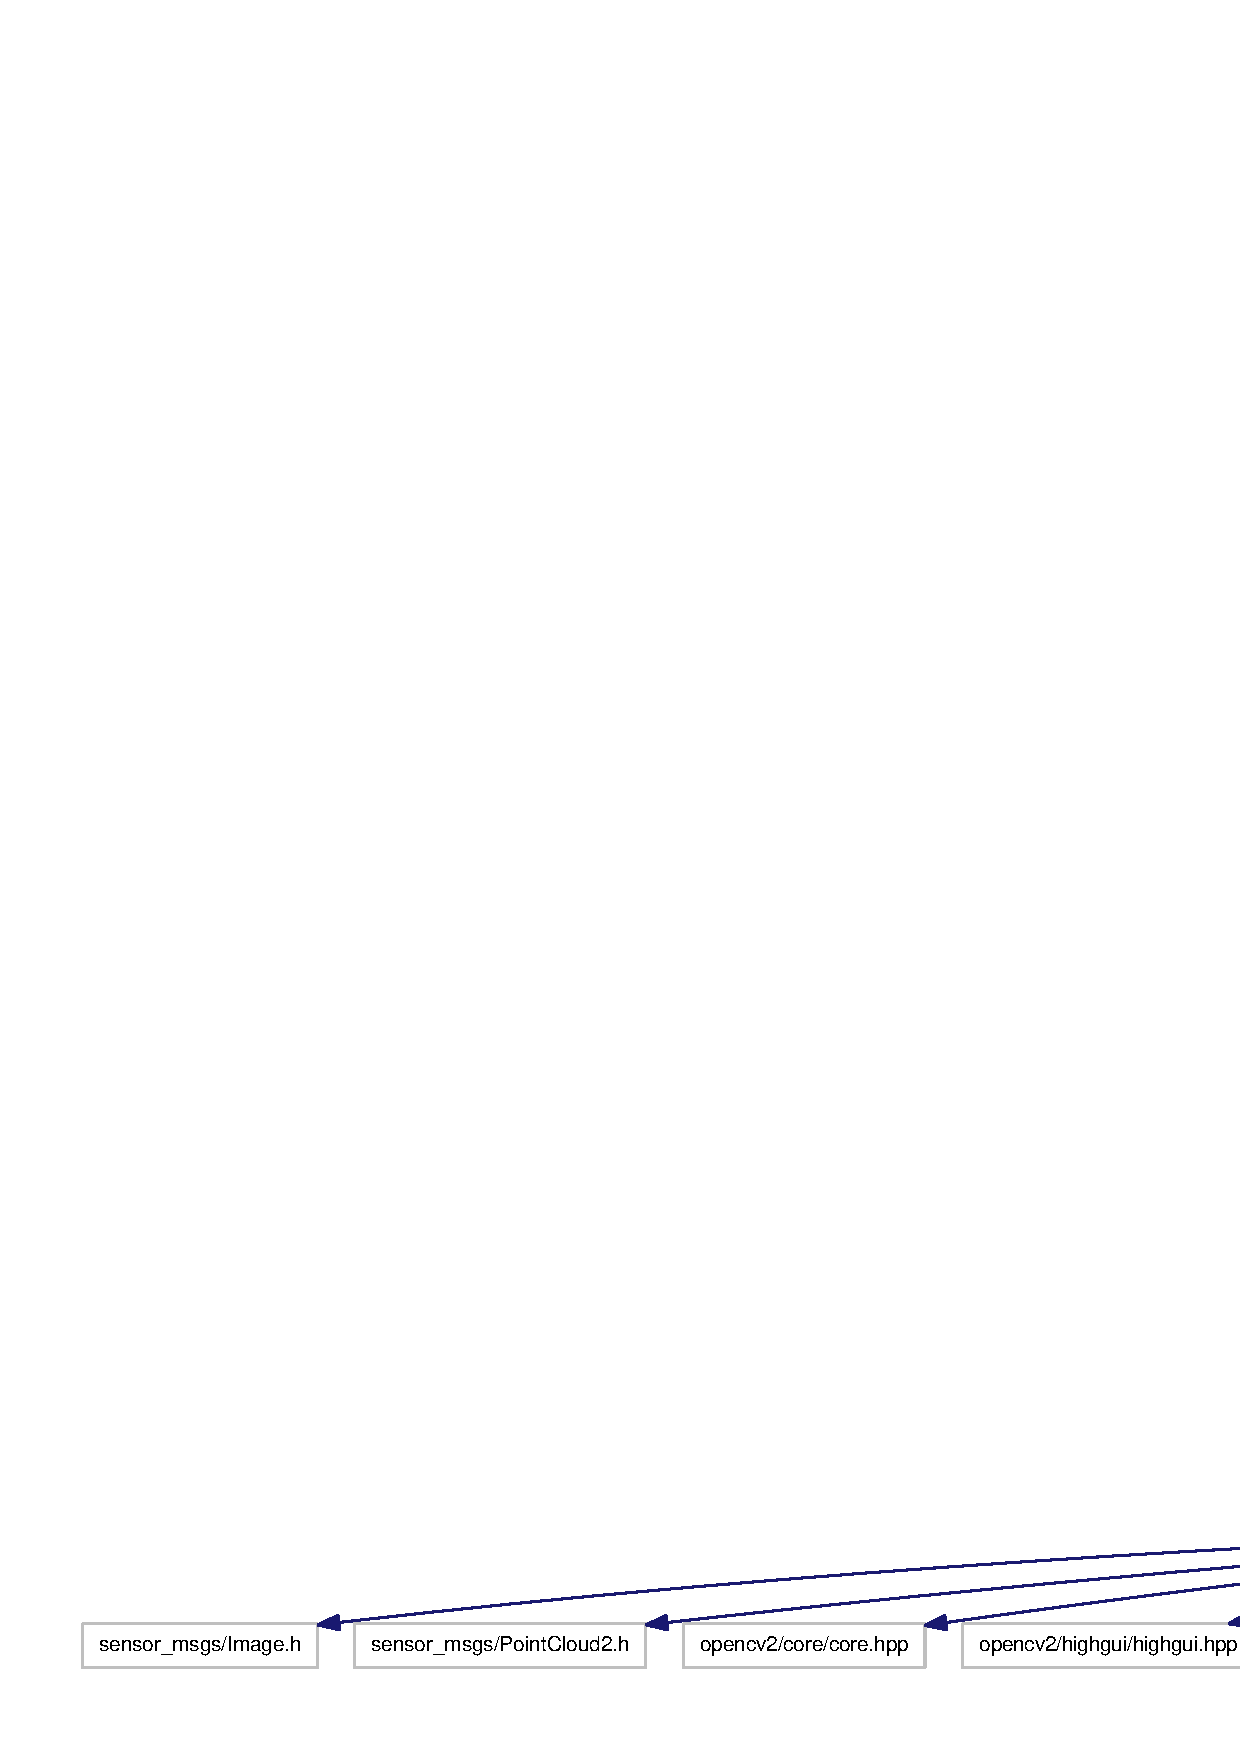
\includegraphics[width=350pt]{sensor__processor_8cpp__incl}
\end{center}
\end{figure}


\subsection{\-Detailed \-Description}

\footnotesize  
\normalsize \begin{DoxyAuthor}{\-Author}
\-George \-Andrew \-Brindeiro ({\tt georgebrindeiro@lara.\-unb.\-br}) 
\end{DoxyAuthor}
\begin{DoxyDate}{\-Date}
\-Apr 22, 2014
\end{DoxyDate}
\begin{DoxyAttention}{\-Attention}
\-Copyright (\-C) 2014 

\-Laboratório de \-Automação e \-Robótica (\-L\-A\-R\-A) 

\-Universidade de \-Brasília (\-Un\-B)
\end{DoxyAttention}
$<$detailed description=\char`\"{}\char`\"{} which=\char`\"{}\char`\"{} may=\char`\"{}\char`\"{} contain=\char`\"{}\char`\"{} examples=\char`\"{}\char`\"{} and=\char`\"{}\char`\"{} test=\char`\"{}\char`\"{} cases$>$=\char`\"{}\char`\"{}$>$ 

\-Definition in file {\bf sensor\-\_\-processor.\-cpp}.


\section{sensor\-\_\-processor.\-h \-File \-Reference}
\label{sensor__processor_8h}\index{sensor\-\_\-processor.\-h@{sensor\-\_\-processor.\-h}}
{\ttfamily \#include $<$sensor\-\_\-msgs/\-Image.\-h$>$}\*
{\ttfamily \#include $<$sensor\-\_\-msgs/\-Point\-Cloud2.\-h$>$}\*
{\ttfamily \#include $<$opencv2/core/core.\-hpp$>$}\*
{\ttfamily \#include $<$opencv2/highgui/highgui.\-hpp$>$}\*
{\ttfamily \#include $<$opencv2/nonfree/features2d.\-hpp$>$}\*
{\ttfamily \#include $<$cv\-\_\-bridge/cv\-\_\-bridge.\-h$>$}\*
{\ttfamily \#include $<$pcl/filters/extract\-\_\-indices.\-h$>$}\*
{\ttfamily \#include $<$pcl/point\-\_\-cloud.\-h$>$}\*
{\ttfamily \#include $<$pcl/point\-\_\-types.\-h$>$}\*
{\ttfamily \#include $<$pcl/ros/conversions.\-h$>$}\*
{\ttfamily \#include $<$pcl\-\_\-conversions/pcl\-\_\-conversions.\-h$>$}\*
\-Include dependency graph for sensor\-\_\-processor.\-h\-:\nopagebreak
\begin{figure}[H]
\begin{center}
\leavevmode
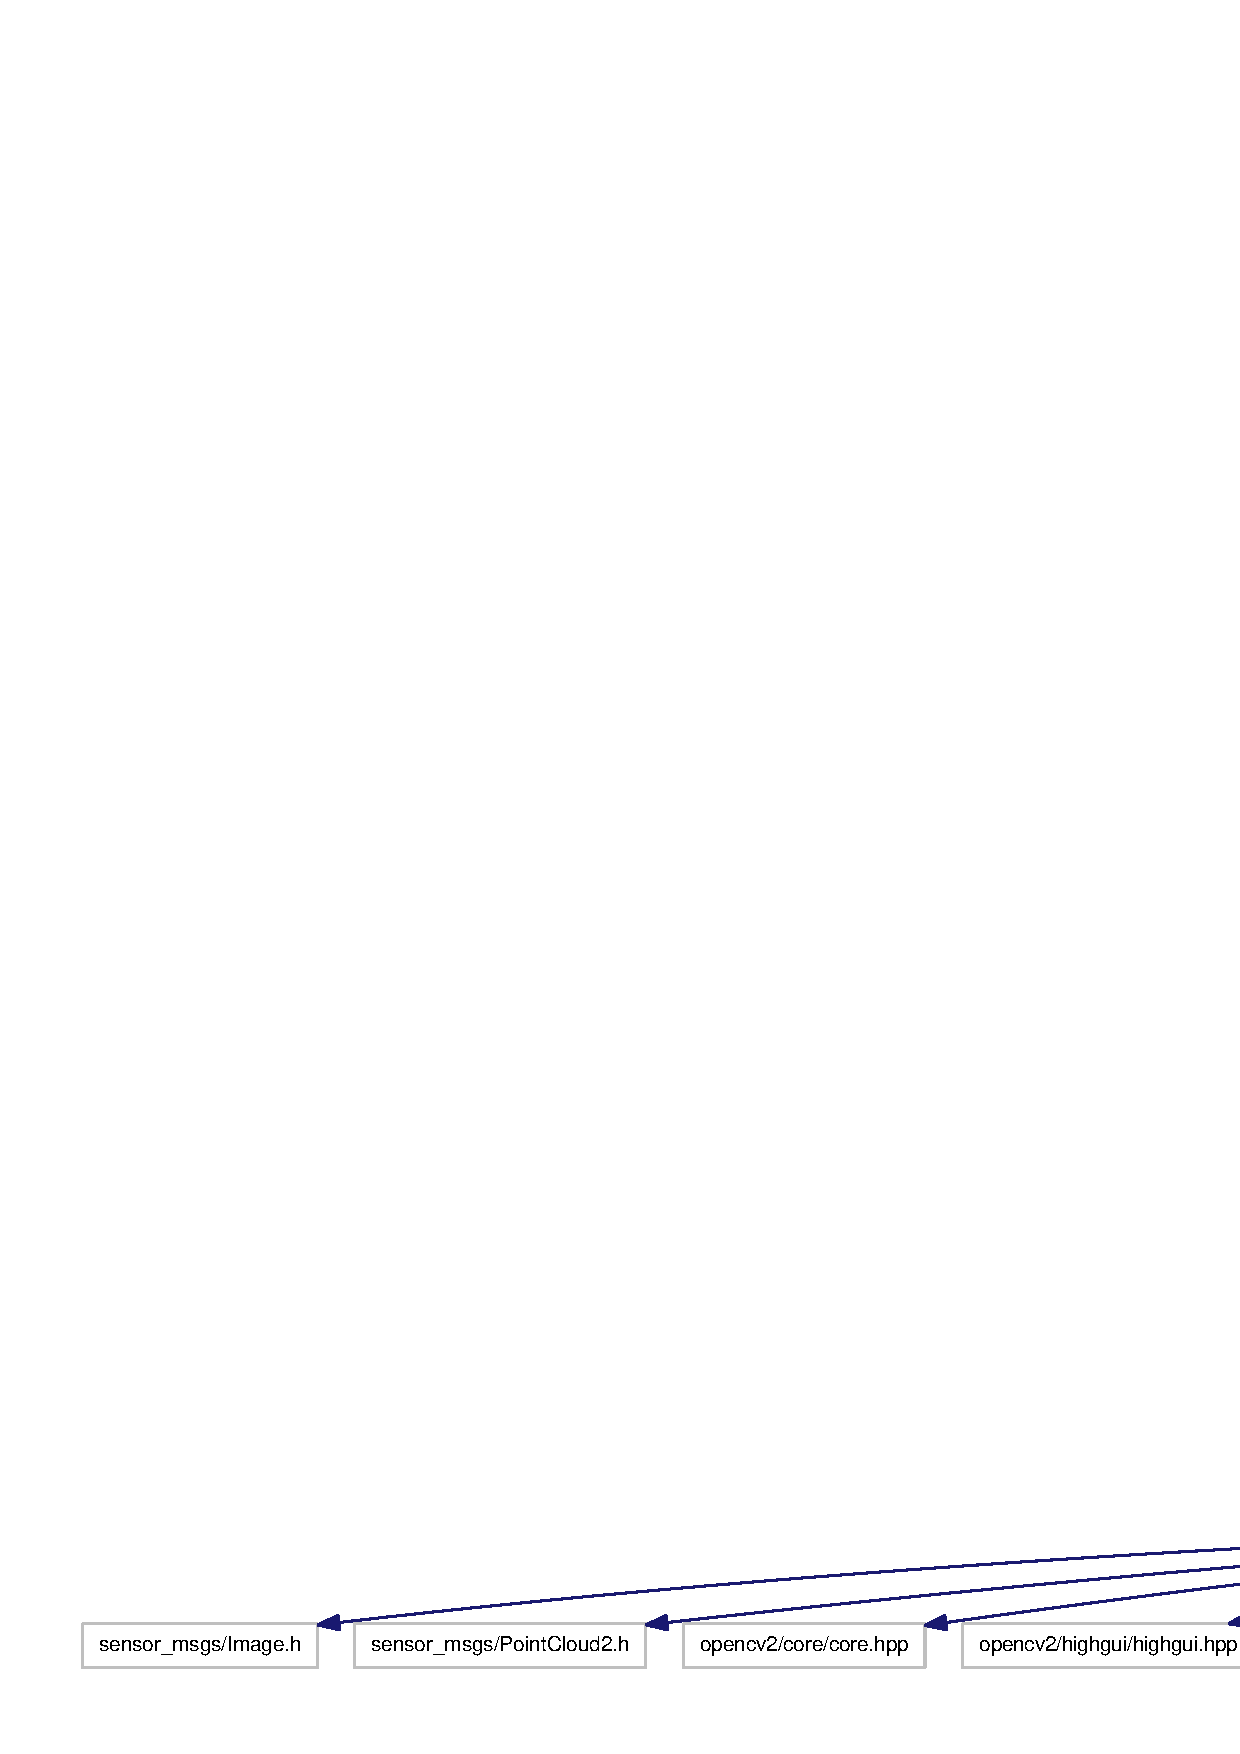
\includegraphics[width=350pt]{sensor__processor_8h__incl}
\end{center}
\end{figure}
\-This graph shows which files directly or indirectly include this file\-:\nopagebreak
\begin{figure}[H]
\begin{center}
\leavevmode
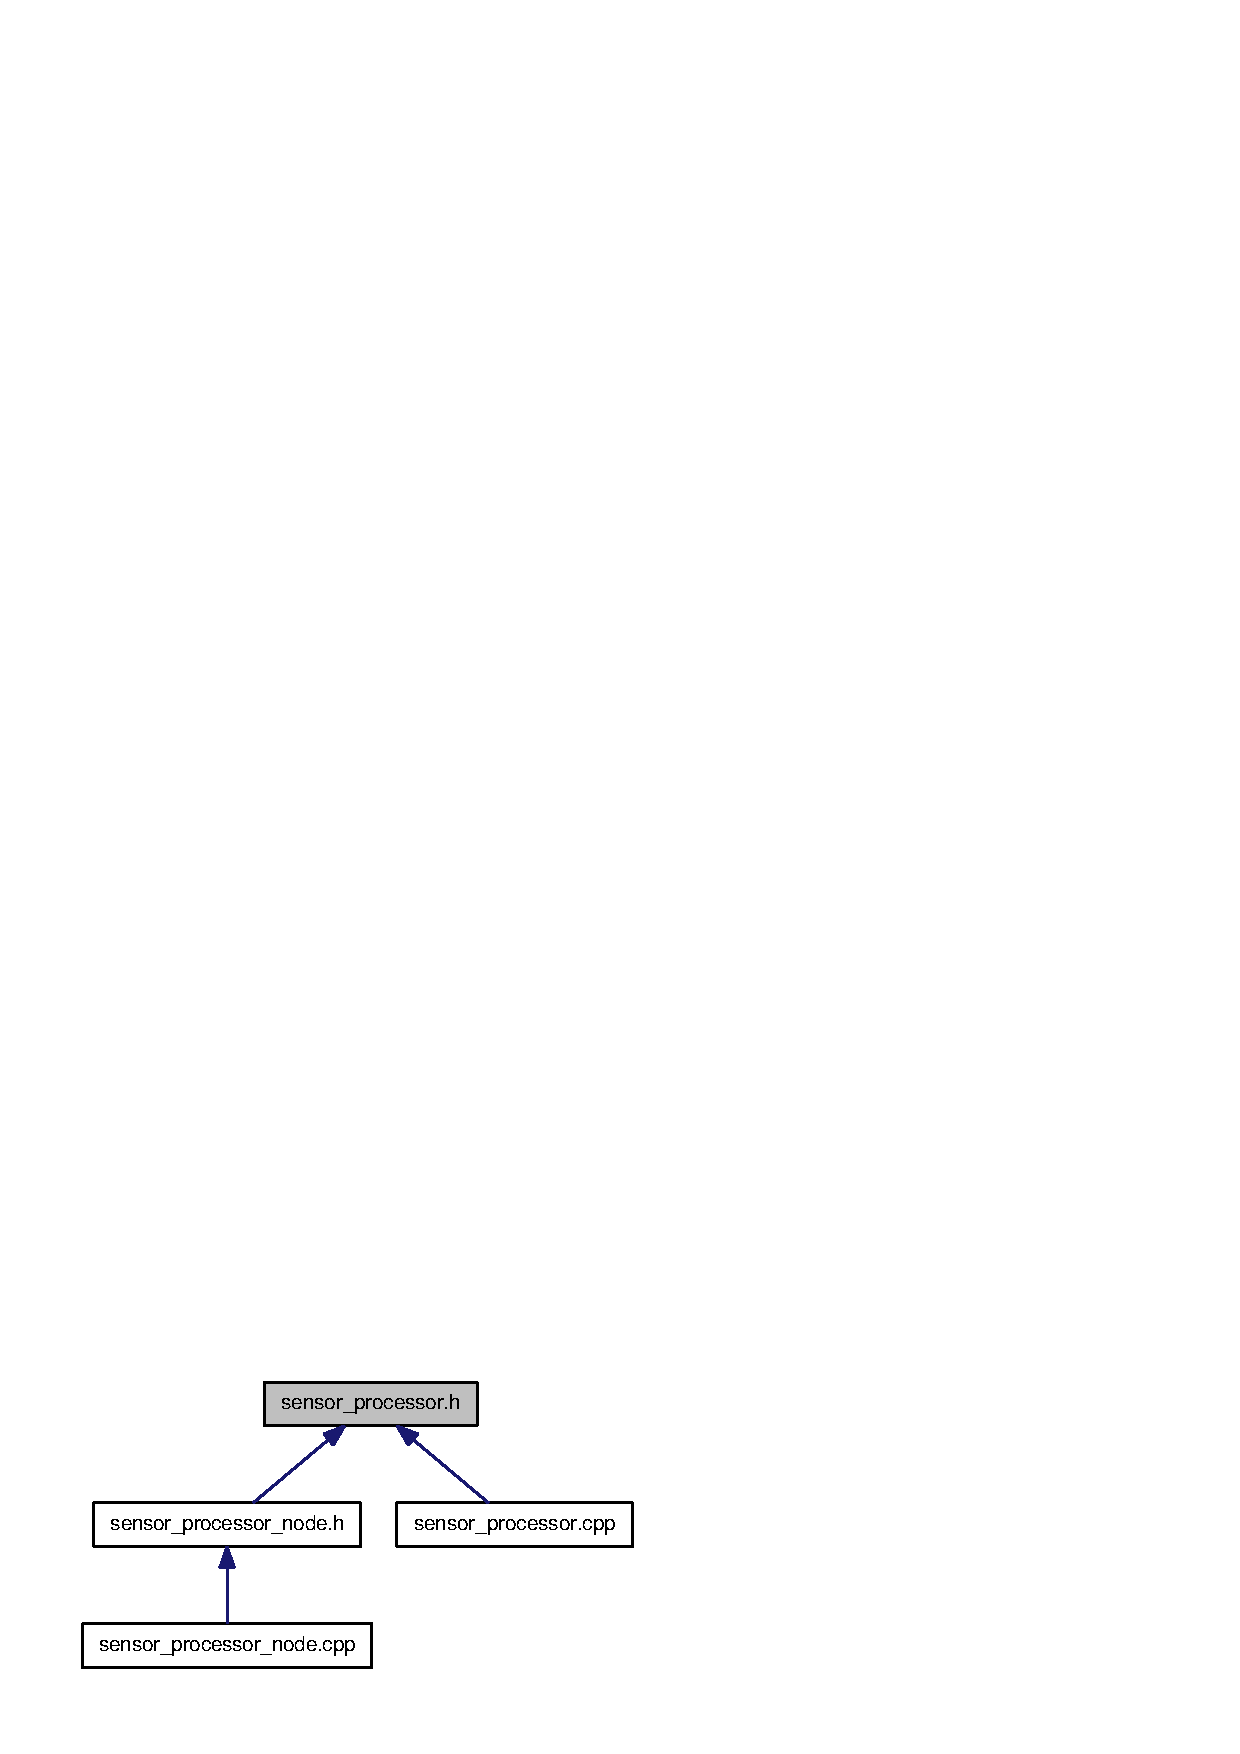
\includegraphics[width=307pt]{sensor__processor_8h__dep__incl}
\end{center}
\end{figure}
\subsection*{\-Classes}
\begin{DoxyCompactItemize}
\item 
class {\bf \-Sensor\-Processor}
\end{DoxyCompactItemize}
\subsection*{\-Enumerations}
\begin{DoxyCompactItemize}
\item 
enum {\bf \-Feature\-Detector} \{ {\bf \-S\-U\-R\-F}
 \}
\end{DoxyCompactItemize}


\subsection{\-Detailed \-Description}
\begin{DoxyAuthor}{\-Author}
\-George \-Andrew \-Brindeiro ({\tt georgebrindeiro@lara.\-unb.\-br}) 
\end{DoxyAuthor}
\begin{DoxyDate}{\-Date}
\-Apr 22, 2014
\end{DoxyDate}
\begin{DoxyAttention}{\-Attention}
\-Copyright (\-C) 2014 

\-Laboratório de \-Automação e \-Robótica (\-L\-A\-R\-A) 

\-Universidade de \-Brasília (\-Un\-B) 
\end{DoxyAttention}


\-Definition in file {\bf sensor\-\_\-processor.\-h}.



\subsection{\-Enumeration \-Type \-Documentation}
\index{sensor\-\_\-processor.\-h@{sensor\-\_\-processor.\-h}!\-Feature\-Detector@{\-Feature\-Detector}}
\index{\-Feature\-Detector@{\-Feature\-Detector}!sensor_processor.h@{sensor\-\_\-processor.\-h}}
\subsubsection[{\-Feature\-Detector}]{\setlength{\rightskip}{0pt plus 5cm}enum {\bf \-Feature\-Detector}}\label{sensor__processor_8h_ae09a21467c8801805113023bd99eeef0}
$<$ \-Feature detectors that can be used in \doxyref{\-Sensor\-Processor}{p.}{classSensorProcessor} \begin{Desc}
\item[\-Enumerator\-: ]\par
\begin{description}
\index{\-S\-U\-R\-F@{\-S\-U\-R\-F}!sensor\-\_\-processor.\-h@{sensor\-\_\-processor.\-h}}\index{sensor\-\_\-processor.\-h@{sensor\-\_\-processor.\-h}!\-S\-U\-R\-F@{\-S\-U\-R\-F}}\item[{\em 
\-S\-U\-R\-F\label{sensor__processor_8h_ae09a21467c8801805113023bd99eeef0a0bbe695c3ec447658d4384c111cead3b}
}]\end{description}
\end{Desc}



\-Definition at line 31 of file sensor\-\_\-processor.\-h.


\section{sensor\-\_\-processor\-\_\-node.\-cpp \-File \-Reference}
\label{sensor__processor__node_8cpp}\index{sensor\-\_\-processor\-\_\-node.\-cpp@{sensor\-\_\-processor\-\_\-node.\-cpp}}


\-R\-O\-S node used to process raw sensor data.  


{\ttfamily \#include $<$ros/ros.\-h$>$}\*
{\ttfamily \#include $<$sensor\-\_\-processor/sensor\-\_\-processor\-\_\-node.\-h$>$}\*
\-Include dependency graph for sensor\-\_\-processor\-\_\-node.\-cpp\-:\nopagebreak
\begin{figure}[H]
\begin{center}
\leavevmode
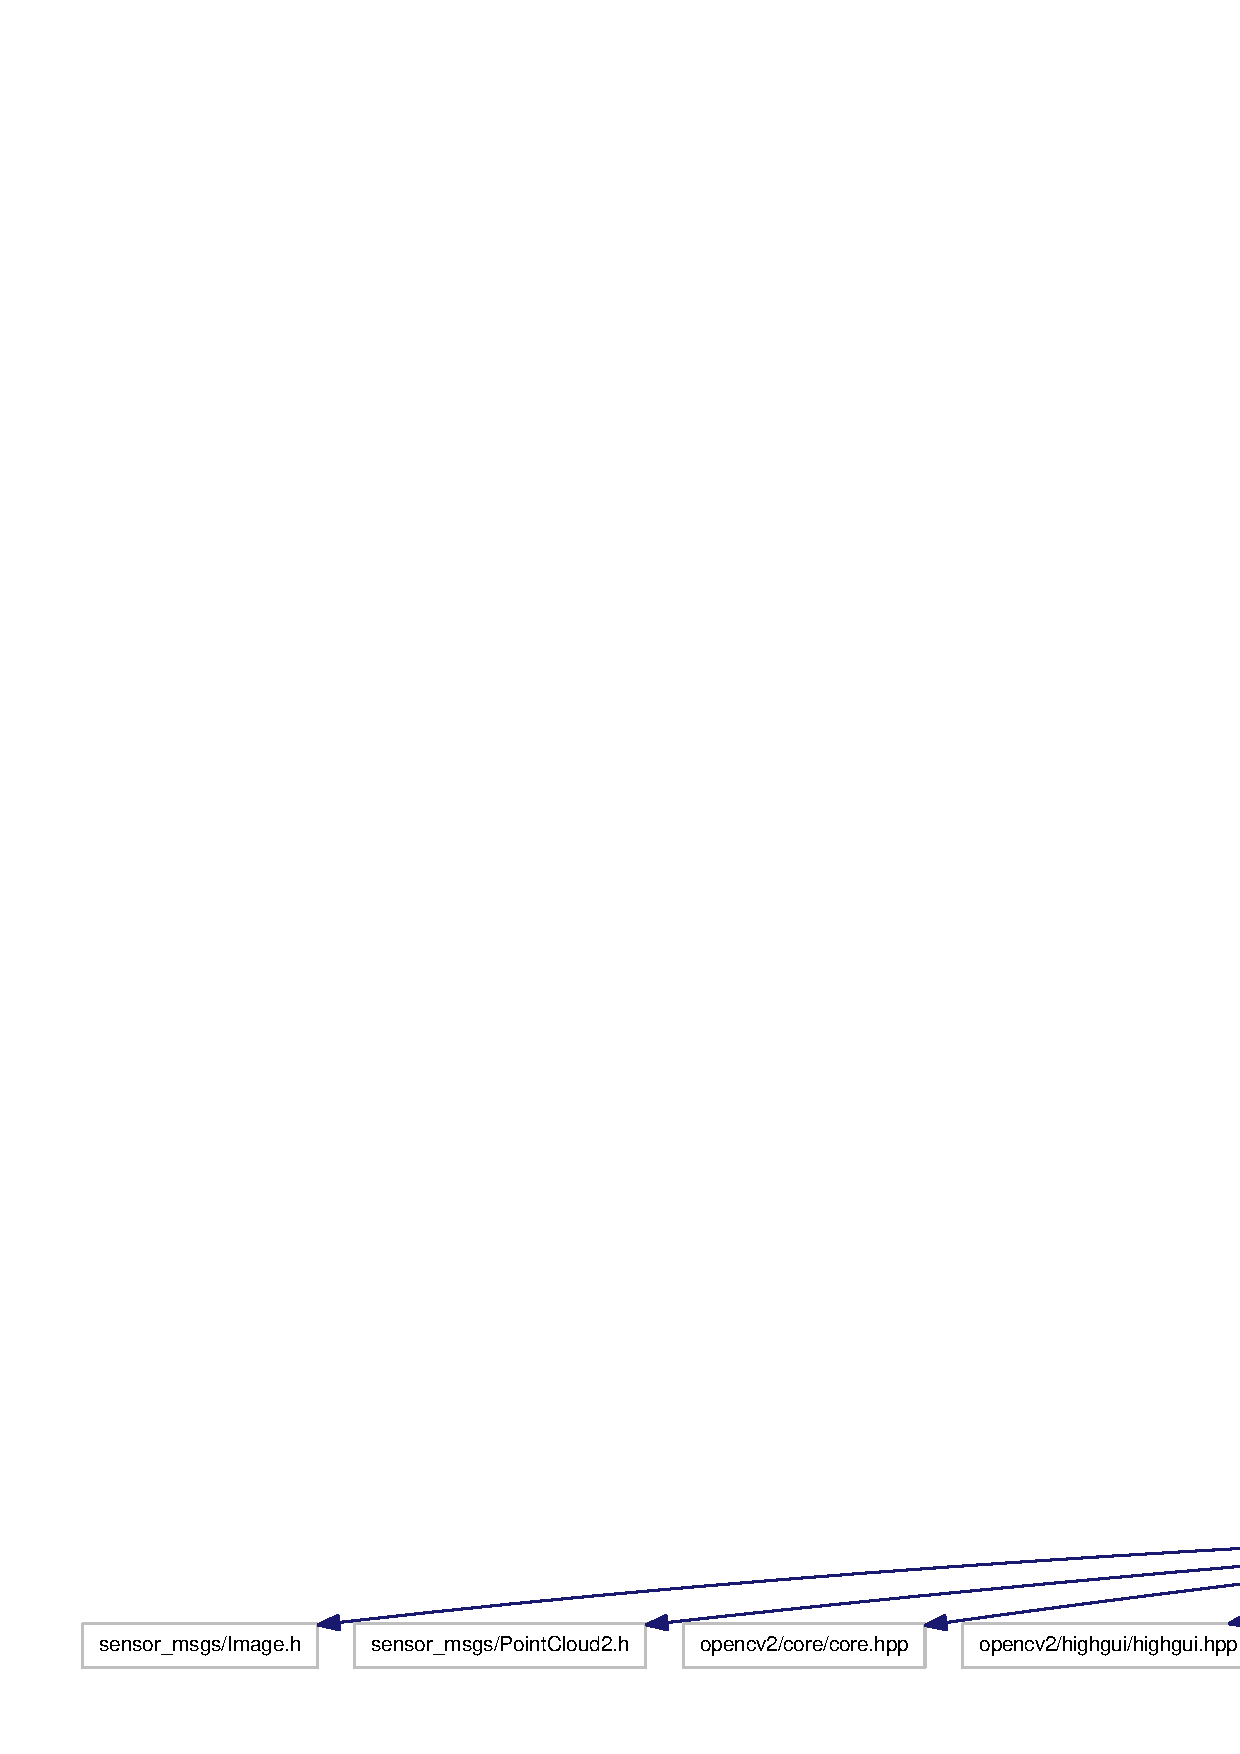
\includegraphics[width=350pt]{sensor__processor__node_8cpp__incl}
\end{center}
\end{figure}
\subsection*{\-Functions}
\begin{DoxyCompactItemize}
\item 
void {\bf cloud\-\_\-cb} (const sensor\-\_\-msgs\-::\-Point\-Cloud2\-::\-Const\-Ptr \&cloud\-\_\-msg)
\item 
int {\bf main} (int argc, char $\ast$$\ast$argv)
\item 
void {\bf odom\-\_\-cb} (const nav\-\_\-msgs\-::\-Odometry\-::\-Const\-Ptr \&odom\-\_\-msg)
\item 
void {\bf print\-\_\-cloud\-\_\-msg} (const sensor\-\_\-msgs\-::\-Point\-Cloud2\-::\-Const\-Ptr \&cloud\-\_\-msg)
\end{DoxyCompactItemize}


\subsection{\-Detailed \-Description}
\-R\-O\-S node used to process raw sensor data. \begin{DoxyAuthor}{\-Author}
\-George \-Andrew \-Brindeiro ({\tt georgebrindeiro@lara.\-unb.\-br}) 
\end{DoxyAuthor}
\begin{DoxyDate}{\-Date}
\-Apr 22, 2014
\end{DoxyDate}
\begin{DoxyAttention}{\-Attention}
\-Copyright (\-C) 2014 

\-Laboratório de \-Automação e \-Robótica (\-L\-A\-R\-A) 

\-Universidade de \-Brasília (\-Un\-B)
\end{DoxyAttention}
\-This \-R\-O\-S node receives both the \-R\-G\-B-\/\-D point cloud from the \-Kinect and the odometry info from the \-Pioneer 

\-Definition in file {\bf sensor\-\_\-processor\-\_\-node.\-cpp}.



\subsection{\-Function \-Documentation}
\index{sensor\-\_\-processor\-\_\-node.\-cpp@{sensor\-\_\-processor\-\_\-node.\-cpp}!cloud\-\_\-cb@{cloud\-\_\-cb}}
\index{cloud\-\_\-cb@{cloud\-\_\-cb}!sensor_processor_node.cpp@{sensor\-\_\-processor\-\_\-node.\-cpp}}
\subsubsection[{cloud\-\_\-cb}]{\setlength{\rightskip}{0pt plus 5cm}void {\bf cloud\-\_\-cb} (
\begin{DoxyParamCaption}
\item[{const sensor\-\_\-msgs\-::\-Point\-Cloud2\-::\-Const\-Ptr \&}]{cloud\-\_\-msg}
\end{DoxyParamCaption}
)}\label{sensor__processor__node_8cpp_a8da8b203137bb48b721ecfe07b875628}


\-Definition at line 42 of file sensor\-\_\-processor\-\_\-node.\-cpp.

\index{sensor\-\_\-processor\-\_\-node.\-cpp@{sensor\-\_\-processor\-\_\-node.\-cpp}!main@{main}}
\index{main@{main}!sensor_processor_node.cpp@{sensor\-\_\-processor\-\_\-node.\-cpp}}
\subsubsection[{main}]{\setlength{\rightskip}{0pt plus 5cm}int {\bf main} (
\begin{DoxyParamCaption}
\item[{int}]{argc, }
\item[{char $\ast$$\ast$}]{argv}
\end{DoxyParamCaption}
)}\label{sensor__processor__node_8cpp_a3c04138a5bfe5d72780bb7e82a18e627}


\-Definition at line 19 of file sensor\-\_\-processor\-\_\-node.\-cpp.

\index{sensor\-\_\-processor\-\_\-node.\-cpp@{sensor\-\_\-processor\-\_\-node.\-cpp}!odom\-\_\-cb@{odom\-\_\-cb}}
\index{odom\-\_\-cb@{odom\-\_\-cb}!sensor_processor_node.cpp@{sensor\-\_\-processor\-\_\-node.\-cpp}}
\subsubsection[{odom\-\_\-cb}]{\setlength{\rightskip}{0pt plus 5cm}void {\bf odom\-\_\-cb} (
\begin{DoxyParamCaption}
\item[{const nav\-\_\-msgs\-::\-Odometry\-::\-Const\-Ptr \&}]{odom\-\_\-msg}
\end{DoxyParamCaption}
)}\label{sensor__processor__node_8cpp_a3ac36cf31bca91aacd880b33c5ec9290}


\-Definition at line 91 of file sensor\-\_\-processor\-\_\-node.\-cpp.

\index{sensor\-\_\-processor\-\_\-node.\-cpp@{sensor\-\_\-processor\-\_\-node.\-cpp}!print\-\_\-cloud\-\_\-msg@{print\-\_\-cloud\-\_\-msg}}
\index{print\-\_\-cloud\-\_\-msg@{print\-\_\-cloud\-\_\-msg}!sensor_processor_node.cpp@{sensor\-\_\-processor\-\_\-node.\-cpp}}
\subsubsection[{print\-\_\-cloud\-\_\-msg}]{\setlength{\rightskip}{0pt plus 5cm}void {\bf print\-\_\-cloud\-\_\-msg} (
\begin{DoxyParamCaption}
\item[{const sensor\-\_\-msgs\-::\-Point\-Cloud2\-::\-Const\-Ptr \&}]{cloud\-\_\-msg}
\end{DoxyParamCaption}
)}\label{sensor__processor__node_8cpp_ac0932d98594119cb7d7388d4c707c8d7}


\-Definition at line 63 of file sensor\-\_\-processor\-\_\-node.\-cpp.


\section{sensor\-\_\-processor\-\_\-node.\-h \-File \-Reference}
\label{sensor__processor__node_8h}\index{sensor\-\_\-processor\-\_\-node.\-h@{sensor\-\_\-processor\-\_\-node.\-h}}
{\ttfamily \#include $<$sensor\-\_\-processor/sensor\-\_\-processor.\-h$>$}\*
{\ttfamily \#include $<$geometry\-\_\-msgs/\-Pose\-With\-Covariance\-Stamped.\-h$>$}\*
{\ttfamily \#include $<$nav\-\_\-msgs/\-Odometry.\-h$>$}\*
\-Include dependency graph for sensor\-\_\-processor\-\_\-node.\-h\-:\nopagebreak
\begin{figure}[H]
\begin{center}
\leavevmode
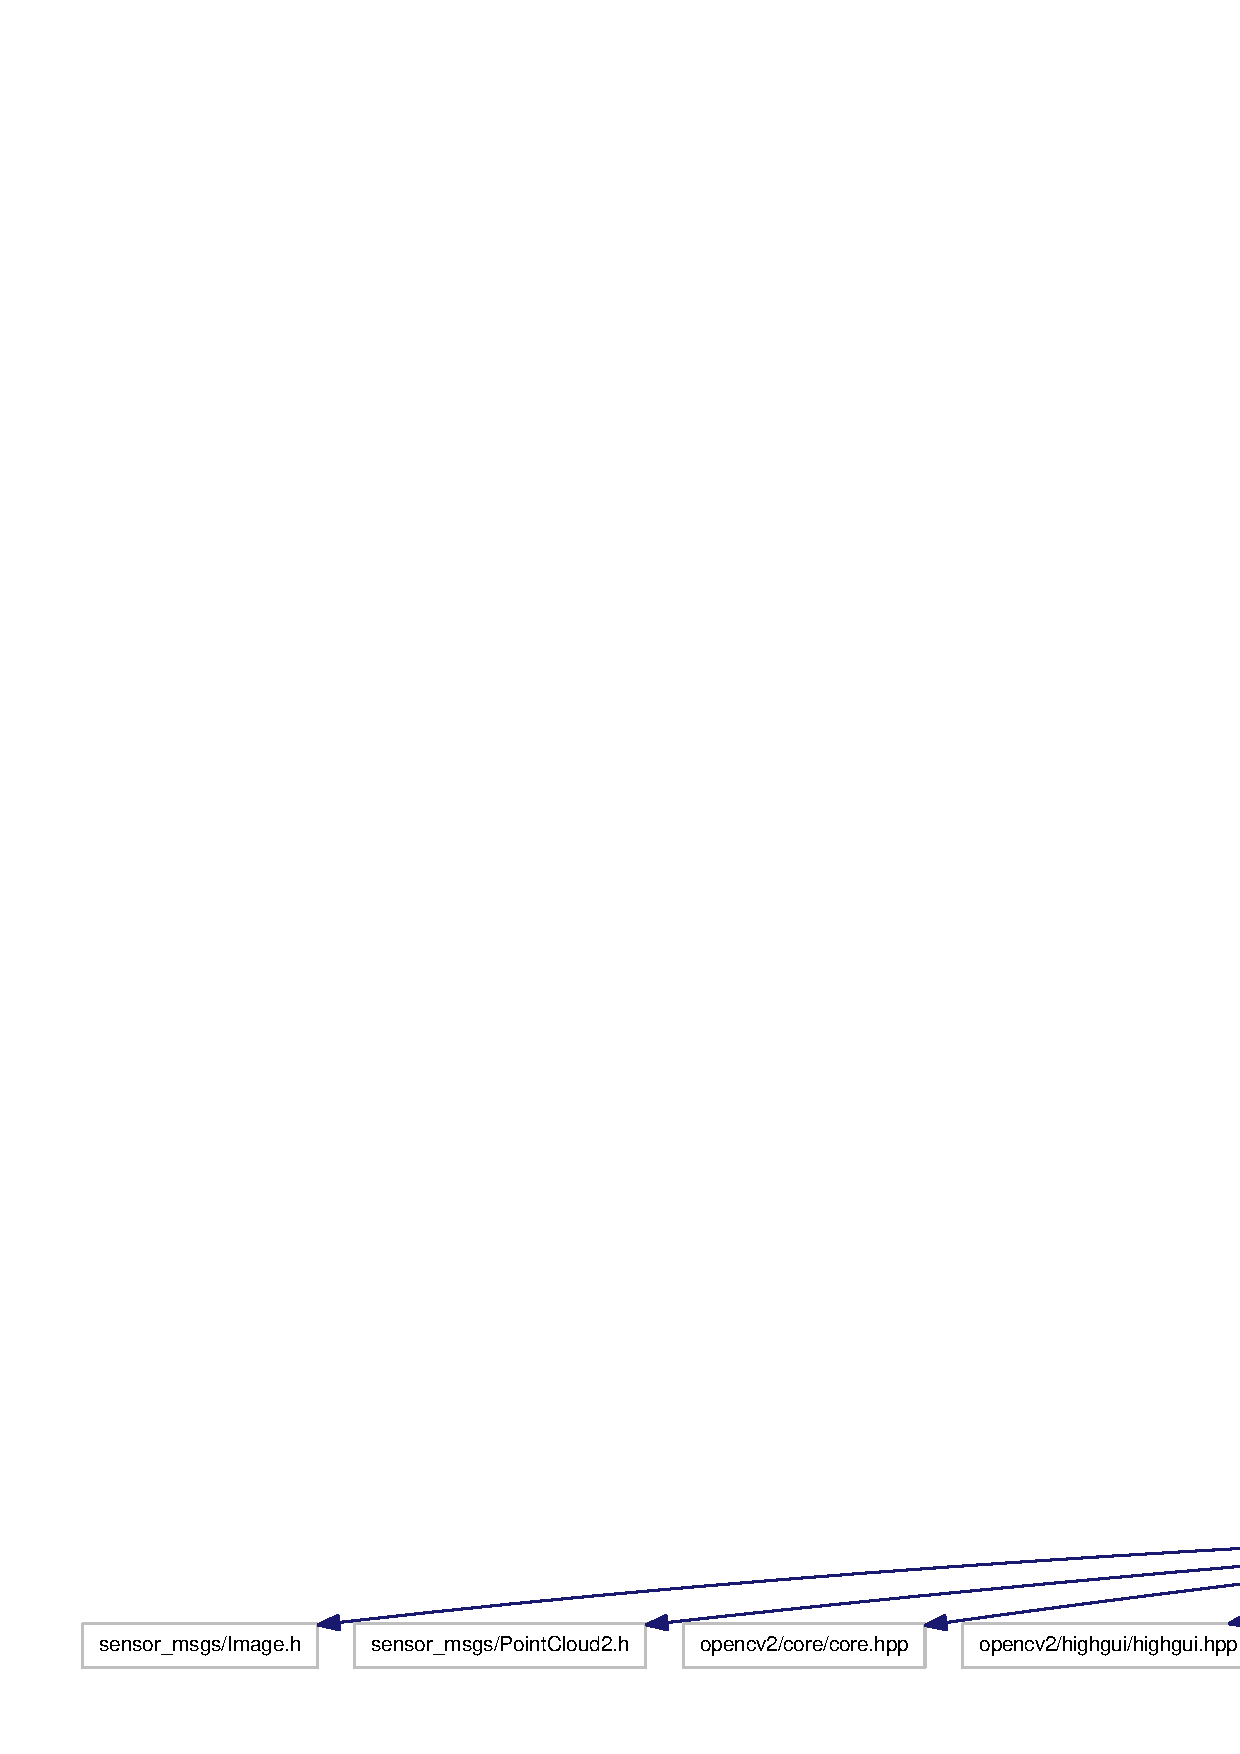
\includegraphics[width=350pt]{sensor__processor__node_8h__incl}
\end{center}
\end{figure}
\-This graph shows which files directly or indirectly include this file\-:\nopagebreak
\begin{figure}[H]
\begin{center}
\leavevmode
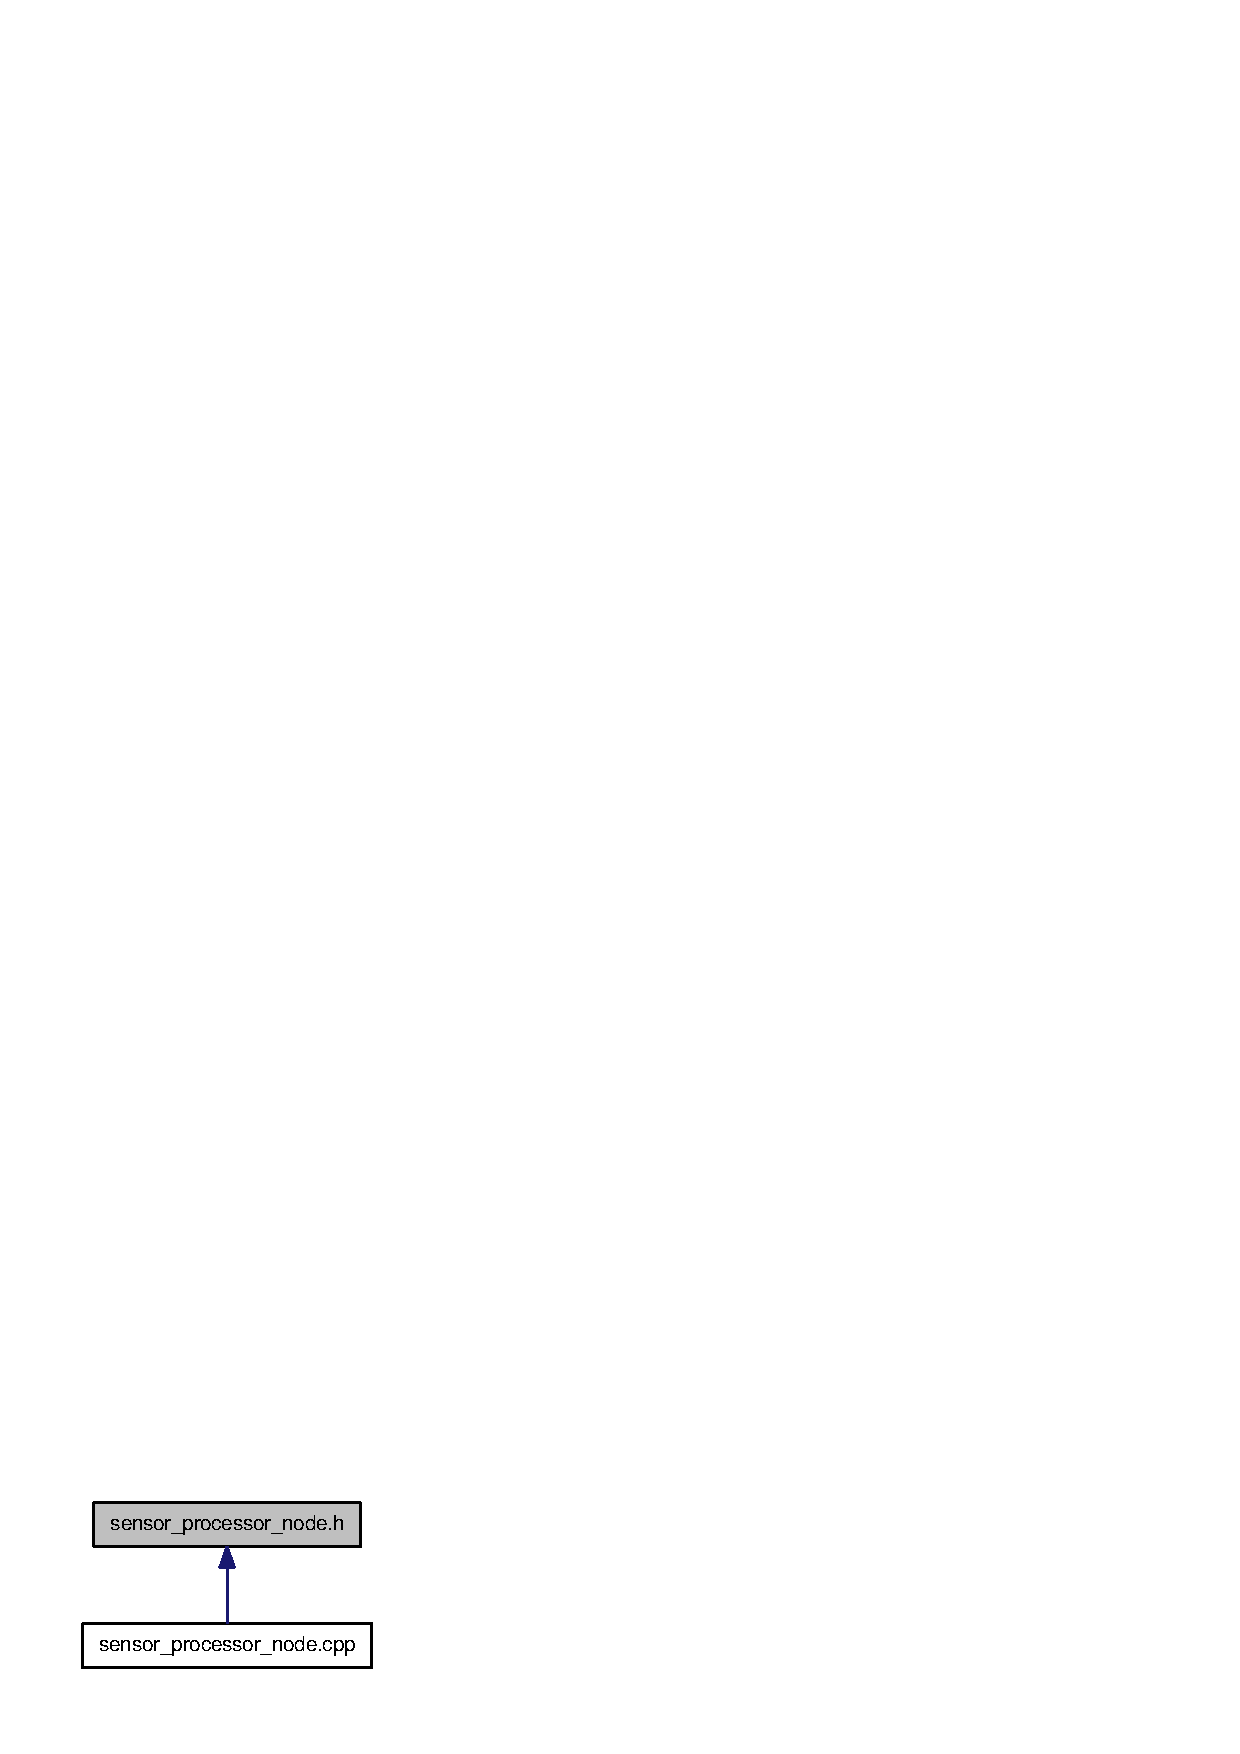
\includegraphics[width=182pt]{sensor__processor__node_8h__dep__incl}
\end{center}
\end{figure}
\subsection*{\-Functions}
\begin{DoxyCompactItemize}
\item 
void {\bf cloud\-\_\-cb} (const sensor\-\_\-msgs\-::\-Point\-Cloud2\-::\-Const\-Ptr \&cloud\-\_\-msg)
\item 
void {\bf odom\-\_\-cb} (const nav\-\_\-msgs\-::\-Odometry\-::\-Const\-Ptr \&odom\-\_\-msg)
\item 
void {\bf print\-\_\-cloud\-\_\-msg} (const sensor\-\_\-msgs\-::\-Point\-Cloud2\-::\-Const\-Ptr \&cloud\-\_\-msg)
\end{DoxyCompactItemize}
\subsection*{\-Variables}
\begin{DoxyCompactItemize}
\item 
ros\-::\-Publisher {\bf pub\-\_\-cloud}
\item 
ros\-::\-Publisher {\bf pub\-\_\-pose}
\item 
{\bf \-Sensor\-Processor} $\ast$ {\bf sensor\-\_\-processor}
\end{DoxyCompactItemize}


\subsection{\-Detailed \-Description}
\begin{DoxyAuthor}{\-Author}
\-George \-Andrew \-Brindeiro ({\tt georgebrindeiro@lara.\-unb.\-br}) 
\end{DoxyAuthor}
\begin{DoxyDate}{\-Date}
\-Apr 22, 2014
\end{DoxyDate}
\begin{DoxyAttention}{\-Attention}
\-Copyright (\-C) 2014 

\-Laboratório de \-Automação e \-Robótica (\-L\-A\-R\-A) 

\-Universidade de \-Brasília (\-Un\-B) 
\end{DoxyAttention}


\-Definition in file {\bf sensor\-\_\-processor\-\_\-node.\-h}.



\subsection{\-Function \-Documentation}
\index{sensor\-\_\-processor\-\_\-node.\-h@{sensor\-\_\-processor\-\_\-node.\-h}!cloud\-\_\-cb@{cloud\-\_\-cb}}
\index{cloud\-\_\-cb@{cloud\-\_\-cb}!sensor_processor_node.h@{sensor\-\_\-processor\-\_\-node.\-h}}
\subsubsection[{cloud\-\_\-cb}]{\setlength{\rightskip}{0pt plus 5cm}void {\bf cloud\-\_\-cb} (
\begin{DoxyParamCaption}
\item[{const sensor\-\_\-msgs\-::\-Point\-Cloud2\-::\-Const\-Ptr \&}]{cloud\-\_\-msg}
\end{DoxyParamCaption}
)}\label{sensor__processor__node_8h_a8da8b203137bb48b721ecfe07b875628}


\-Definition at line 42 of file sensor\-\_\-processor\-\_\-node.\-cpp.

\index{sensor\-\_\-processor\-\_\-node.\-h@{sensor\-\_\-processor\-\_\-node.\-h}!odom\-\_\-cb@{odom\-\_\-cb}}
\index{odom\-\_\-cb@{odom\-\_\-cb}!sensor_processor_node.h@{sensor\-\_\-processor\-\_\-node.\-h}}
\subsubsection[{odom\-\_\-cb}]{\setlength{\rightskip}{0pt plus 5cm}void {\bf odom\-\_\-cb} (
\begin{DoxyParamCaption}
\item[{const nav\-\_\-msgs\-::\-Odometry\-::\-Const\-Ptr \&}]{odom\-\_\-msg}
\end{DoxyParamCaption}
)}\label{sensor__processor__node_8h_a3ac36cf31bca91aacd880b33c5ec9290}


\-Definition at line 91 of file sensor\-\_\-processor\-\_\-node.\-cpp.

\index{sensor\-\_\-processor\-\_\-node.\-h@{sensor\-\_\-processor\-\_\-node.\-h}!print\-\_\-cloud\-\_\-msg@{print\-\_\-cloud\-\_\-msg}}
\index{print\-\_\-cloud\-\_\-msg@{print\-\_\-cloud\-\_\-msg}!sensor_processor_node.h@{sensor\-\_\-processor\-\_\-node.\-h}}
\subsubsection[{print\-\_\-cloud\-\_\-msg}]{\setlength{\rightskip}{0pt plus 5cm}void {\bf print\-\_\-cloud\-\_\-msg} (
\begin{DoxyParamCaption}
\item[{const sensor\-\_\-msgs\-::\-Point\-Cloud2\-::\-Const\-Ptr \&}]{cloud\-\_\-msg}
\end{DoxyParamCaption}
)}\label{sensor__processor__node_8h_ac0932d98594119cb7d7388d4c707c8d7}


\-Definition at line 63 of file sensor\-\_\-processor\-\_\-node.\-cpp.



\subsection{\-Variable \-Documentation}
\index{sensor\-\_\-processor\-\_\-node.\-h@{sensor\-\_\-processor\-\_\-node.\-h}!pub\-\_\-cloud@{pub\-\_\-cloud}}
\index{pub\-\_\-cloud@{pub\-\_\-cloud}!sensor_processor_node.h@{sensor\-\_\-processor\-\_\-node.\-h}}
\subsubsection[{pub\-\_\-cloud}]{\setlength{\rightskip}{0pt plus 5cm}ros\-::\-Publisher {\bf pub\-\_\-cloud}}\label{sensor__processor__node_8h_a6600fdbe96f8c1420ee414ba41c90027}


\-Definition at line 19 of file sensor\-\_\-processor\-\_\-node.\-h.

\index{sensor\-\_\-processor\-\_\-node.\-h@{sensor\-\_\-processor\-\_\-node.\-h}!pub\-\_\-pose@{pub\-\_\-pose}}
\index{pub\-\_\-pose@{pub\-\_\-pose}!sensor_processor_node.h@{sensor\-\_\-processor\-\_\-node.\-h}}
\subsubsection[{pub\-\_\-pose}]{\setlength{\rightskip}{0pt plus 5cm}ros\-::\-Publisher {\bf pub\-\_\-pose}}\label{sensor__processor__node_8h_a1a081b07689cdd9efdbb2a06f698ec48}


\-Definition at line 29 of file sensor\-\_\-processor\-\_\-node.\-h.

\index{sensor\-\_\-processor\-\_\-node.\-h@{sensor\-\_\-processor\-\_\-node.\-h}!sensor\-\_\-processor@{sensor\-\_\-processor}}
\index{sensor\-\_\-processor@{sensor\-\_\-processor}!sensor_processor_node.h@{sensor\-\_\-processor\-\_\-node.\-h}}
\subsubsection[{sensor\-\_\-processor}]{\setlength{\rightskip}{0pt plus 5cm}{\bf \-Sensor\-Processor}$\ast$ {\bf sensor\-\_\-processor}}\label{sensor__processor__node_8h_a1183caf02d6ec81cc2845ec1c58bd606}


\-Definition at line 21 of file sensor\-\_\-processor\-\_\-node.\-h.


\printindex
\end{document}
